%----------------------------------------------------------------------------------------
%    PACKAGES AND THEMES
%----------------------------------------------------------------------------------------

\documentclass[aspectratio=169,xcolor=dvipsnames]{beamer}
\usetheme{SimplePlus}

\usepackage{hyperref}
\usepackage{graphicx}
\usepackage{booktabs}
\usepackage{amsmath,amssymb,amsfonts}
\usepackage{multirow}
\usepackage{array}
\usepackage{pifont}
\usepackage{adjustbox}
\usepackage{longtable}
% \usepackage{enumitem}  % 已注释：与 Beamer 冲突，Beamer 有自己的列表管理
\usepackage{tikz}
\usetikzlibrary{positioning,arrows.meta,shapes.geometric,calc}
\usepackage[backend=bibtex,style=numeric,sorting=none,natbib=true]{biblatex}
\addbibresource{reference.bib}

% Beamer settings
\setbeamertemplate{bibliography item}{\insertbiblabel}
\renewcommand*{\bibfont}{\scriptsize}

%----------------------------------------------------------------------------------------
%    TITLE PAGE
%----------------------------------------------------------------------------------------

\title{Verdant-Search: Bridging Vision and Text in Distributed Search Through Multimodal Learning-to-Rank}

\author{
    \textbf{Student:} CAI HONGYI, S2175463 \\[0.3em]
    \textbf{Supervisor:} CHIAM YIN KIA
}

\institute{University of Malaya}
\date{\today}

%----------------------------------------------------------------------------------------
%    PRESENTATION SLIDES
%----------------------------------------------------------------------------------------

\begin{document}

\begin{frame}
    \titlepage
\end{frame}

\begin{frame}{Overview}
    \tableofcontents
\end{frame}

%------------------------------------------------
\section{Introduction}
%------------------------------------------------

\begin{frame}{Introduction: The Multimodal Search Gap}
    \begin{columns}[t]
        \column{.48\textwidth}
        \textbf{Enterprise Documents Are Multimodal}
        \begin{itemize}
            \item Business reports, technical docs contain critical visual information
            \item Charts, tables, diagrams convey key insights beyond text
        \end{itemize}
        
        \vspace{1em}
        \textbf{Current Search Systems Are Text Only}
        \begin{itemize}
            \item Commercial solutions ignore visual text mixed content
            \item Reranking methods (RankZephyr, classical LTR) operate purely on text
        \end{itemize}
        
        \column{.48\textwidth}
        \textbf{RAG Systems Lack Iterative Refinement}
        \begin{itemize}
            \item Limited mechanism for LLM insights to improve retrieval
            \item Static search without conversational optimization
        \end{itemize}
        
        \vspace{1em}
        \begin{alertblock}{Core Needs}
            \begin{itemize}
                \item Fast, scalable search over million document collections
                \item Rank documents considering text and visual quality
                \item Conversational AI that actively improves search
            \end{itemize}
        \end{alertblock}
    \end{columns}
\end{frame}

%------------------------------------------------
\section{Problem Statement and Objectives}
%------------------------------------------------

\begin{frame}{Problem Statement}
    \small
    \begin{table}
        \centering
        \renewcommand{\arraystretch}{1.4}
        \begin{tabular}{p{0.08\textwidth}|p{0.85\textwidth}}
        \toprule
        \textbf{ID} & \textbf{Problem Description} \\
        \midrule
        \textbf{P1} & \textbf{Scalability Challenges in Multimodal Search.} Multimodal search requires expensive vision language inference and coordinated indexing. Without proper optimization, systems struggle to achieve subsecond latency at enterprise scale. \\
        \midrule
        \textbf{P2} & \textbf{Absence of Multimodal Reranking.} All existing learning to rank methods process only text. Current approaches lack listwise reasoning over cross modal evidence, leaving visual content unranked. \\
        \midrule
        \textbf{P3} & \textbf{Limited Enterprise Knowledge Access.} Organizations lack bidirectional integration where search improves AI responses and AI insights refine search. Current RAG systems treat retrieval as one shot preprocessing. \\
        \bottomrule
        \end{tabular}
    \end{table}
\end{frame}

\begin{frame}{Research Objectives}
    \begin{table}
        \centering
        \renewcommand{\arraystretch}{1.6}
        \begin{tabular}{p{0.08\textwidth}|p{0.85\textwidth}}
        \toprule
        \textbf{ID} & \textbf{Objective Description} \\
        \midrule
        \textbf{O1} & To identify existing search engine architectures, learning to rank approaches, vision language models, and retrieval augmented generation techniques through literature review. \\
        \midrule
        \textbf{O2} & To design and develop a multimodal search engine integrating distributed crawling, hybrid retrieval, multimodal listwise reranking, and iterative RAG with query rewriting. \\
        \midrule
        \textbf{O3} & To evaluate system effectiveness through ranking metrics, latency benchmarks, and answer quality assessments. \\
        \bottomrule
        \end{tabular}
    \end{table}
\end{frame}

%------------------------------------------------
\section{Literature Review}
%------------------------------------------------

\begin{frame}{Literature Review: Search Engine Architecture (1/9)}
    \scriptsize
    \begin{table}
        \centering
        \renewcommand{\arraystretch}{1.1}
        \begin{tabular}{p{0.18\textwidth}|p{0.35\textwidth}|p{0.35\textwidth}}
        \toprule
        \textbf{Approach} & \textbf{Key Contributions} & \textbf{Limitations} \\
        \midrule
        PageRank \cite{page1999pagerank} & Link based quality indicators; revolutionized web search ranking & Requires link structure; susceptible to manipulation \\
        \midrule
        Tripartite Architecture \cite{brin1998anatomy} & Crawlers, indexers, query processors framework & Text only; single modality \\
        \midrule
        Inverted Index \cite{zobel2006inverted} & Efficient keyword search at web scale; posting lists & Lexical matching only \\
        \midrule
        Neural IR \cite{mitra2017neural} & Semantic understanding beyond keyword matching & Computational overhead \\
        \midrule
        Dense Passage Retrieval \cite{karpukhin2020dense} & BERT based semantic search; zero lexical overlap retrieval & Training data requirements \\
        \bottomrule
        \end{tabular}
    \end{table}
    
    \vspace{0.3em}
    \begin{block}{Selection Rationale}
        \textbf{Selected:} Hybrid architecture combining inverted index (BM25) with dense retrieval (DPR). \\
        \textbf{Reason:} Combines efficiency of keyword search with semantic understanding. Pure keyword methods miss semantic matches; pure neural methods have high latency.
    \end{block}
\end{frame}

\begin{frame}{Literature Review: Keyword Based Search Methods (2/9)}
    \scriptsize
    \begin{table}
        \centering
        \renewcommand{\arraystretch}{1.1}
        \begin{tabular}{p{0.15\textwidth}|p{0.25\textwidth}|p{0.25\textwidth}|p{0.22\textwidth}}
        \toprule
        \textbf{Method} & \textbf{Mechanism} & \textbf{Strength} & \textbf{Weakness} \\
        \midrule
        TF IDF \cite{sparck1972statistical} & Term frequency inverse document frequency weighting & Simple, interpretable & Length bias \\
        \midrule
        BM25 \cite{robertson2009probabilistic} & Probabilistic with saturation and length normalization & Robust baseline; tunable parameters & Lexical gap \\
        \midrule
        Contriever \cite{izacard2022unsupervised} & Unsupervised contrastive dense retrieval & No labeled data needed & Less effective than supervised \\
        \bottomrule
        \end{tabular}
    \end{table}
    
    \vspace{0.3em}
    \begin{block}{Selection Rationale}
        \textbf{Selected:} BM25 for first stage keyword retrieval. \\
        \textbf{Reason:} BM25 remains competitive with neural methods on many benchmarks while offering millisecond latency. TF IDF lacks saturation handling; Contriever requires GPU inference for first stage.
    \end{block}
\end{frame}

\begin{frame}{Literature Review: Vector Embeddings (3/9)}
    \scriptsize
    \begin{table}
        \centering
        \renewcommand{\arraystretch}{1.1}
        \begin{tabular}{p{0.18\textwidth}|p{0.30\textwidth}|p{0.20\textwidth}|p{0.20\textwidth}}
        \toprule
        \textbf{Model} & \textbf{Architecture} & \textbf{Strength} & \textbf{Weakness} \\
        \midrule
        Word2Vec \cite{mikolov2013efficient} & Skip gram, CBOW & Fast training; captures analogies & Context independent \\
        \midrule
        GloVe \cite{pennington2014glove} & Global matrix factorization & Leverages corpus statistics & Static embeddings \\
        \midrule
        BERT \cite{devlin2019bert} & Bidirectional transformer & Deep contextualization & Expensive inference \\
        \midrule
        Sentence BERT \cite{reimers2019sentence} & Siamese BERT & Efficient similarity & Fixed representation \\
        \midrule
        ColBERT \cite{khattab2020colbert} & Late interaction & Fine grained matching & Storage overhead \\
        \bottomrule
        \end{tabular}
    \end{table}
    
    \vspace{0.3em}
    \begin{block}{Selection Rationale}
        \textbf{Selected:} Sentence BERT for text embeddings; CLIP for multimodal alignment. \\
        \textbf{Reason:} Sentence BERT balances quality and efficiency for text. ColBERT has high storage costs. Word2Vec and GloVe lack contextualization needed for semantic search.
    \end{block}
\end{frame}

\begin{frame}{Literature Review: Approximate Nearest Neighbor (4/9)}
    \scriptsize
    \begin{table}
        \centering
        \renewcommand{\arraystretch}{1.1}
        \begin{tabular}{p{0.18\textwidth}|p{0.22\textwidth}|p{0.22\textwidth}|p{0.25\textwidth}}
        \toprule
        \textbf{Algorithm} & \textbf{Index Structure} & \textbf{Query Complexity} & \textbf{Trade off} \\
        \midrule
        Brute Force KNN & None & O(N) & Exact but slow \\
        \midrule
        Product Quantization \cite{jegou2011product} & Learned codebooks & O(N) with fast distance & Memory vs accuracy \\
        \midrule
        IVF & Inverted file clusters & O(N/k) & Partition quality critical \\
        \midrule
        HNSW \cite{malkov2018efficient} & Hierarchical proximity graphs & O(log N) & Build time vs query speed \\
        \midrule
        ANCE \cite{xiong2021approximate} & Hard negative mining & Training time & Improved recall \\
        \bottomrule
        \end{tabular}
    \end{table}
    
    \vspace{0.3em}
    \begin{block}{Selection Rationale}
        \textbf{Selected:} HNSW for vector search index. \\
        \textbf{Reason:} HNSW achieves logarithmic query complexity with high recall. IVF requires careful cluster tuning; PQ trades too much accuracy for memory. HNSW is the industry standard for production vector search.
    \end{block}
\end{frame}

\begin{frame}{Literature Review: Classical Learning to Rank (5/9)}
    \scriptsize
    \begin{table}
        \centering
        \renewcommand{\arraystretch}{1.05}
        \begin{tabular}{p{0.12\textwidth}|p{0.12\textwidth}|p{0.22\textwidth}|p{0.20\textwidth}|p{0.20\textwidth}}
        \toprule
        \textbf{Method} & \textbf{Paradigm} & \textbf{Loss Function} & \textbf{Strength} & \textbf{Weakness} \\
        \midrule
        Regression & Pointwise & MSE & Simple & Ignores ordering \\
        \midrule
        RankNet \cite{burges2005learning} & Pairwise & Pairwise cross entropy & Relative preferences & Quadratic pairs \\
        \midrule
        LambdaRank \cite{burges2006learning} & Pairwise & NDCG gradient & Direct metric optimization & Complex gradients \\
        \midrule
        LambdaMART \cite{burges2010ranknet} & Pairwise & Boosted trees & Robust; interpretable & Feature engineering \\
        \midrule
        ListNet \cite{cao2007learning} & Listwise & Top one probability & Full list context & Permutation cost \\
        \midrule
        ListMLE \cite{xia2008listwise} & Listwise & MLE over permutations & Principled & Computational \\
        \bottomrule
        \end{tabular}
    \end{table}
    
    \vspace{0.3em}
    \begin{block}{Selection Rationale}
        \textbf{Selected:} Listwise paradigm for reranking (extended to LLM based). \\
        \textbf{Reason:} Listwise methods consider full ranking context. LambdaMART requires extensive feature engineering; pointwise ignores document relationships. Listwise enables direct metric optimization.
    \end{block}
\end{frame}

\begin{frame}{Literature Review: LLM Based Ranking (6/9)}
    \scriptsize
    \begin{table}
        \centering
        \renewcommand{\arraystretch}{1.1}
        \begin{tabular}{p{0.18\textwidth}|p{0.25\textwidth}|p{0.22\textwidth}|p{0.22\textwidth}}
        \toprule
        \textbf{Method} & \textbf{Approach} & \textbf{Strength} & \textbf{Weakness} \\
        \midrule
        monoBERT \cite{nogueira2019passage} & Cross encoder scoring & High accuracy & O(N) inference \\
        \midrule
        RankGPT \cite{sun2023chatgpt} & GPT 4 permutation generation & Zero shot; SOTA & High API cost; latency \\
        \midrule
        RankZephyr \cite{pradeep2023rankzephyr} & Distilled setwise prompting & Efficient; open source & Requires fine tuning \\
        \midrule
        Pairwise LLM \cite{qin2023pairwise} & LLM pairwise comparison & Effective & Quadratic comparisons \\
        \bottomrule
        \end{tabular}
    \end{table}
    
    \vspace{0.3em}
    \begin{block}{Selection Rationale}
        \textbf{Selected:} RankZephyr style setwise prompting extended to multimodal. \\
        \textbf{Reason:} RankZephyr balances effectiveness with efficiency through setwise comparison. RankGPT is too expensive for production; pairwise methods have quadratic complexity. Setwise enables listwise ranking with bounded comparisons.
    \end{block}
\end{frame}

\begin{frame}{Literature Review: Vision Language Models (7/9)}
    \scriptsize
    \begin{table}
        \centering
        \renewcommand{\arraystretch}{1.05}
        \begin{tabular}{p{0.12\textwidth}|p{0.20\textwidth}|p{0.18\textwidth}|p{0.18\textwidth}|p{0.18\textwidth}}
        \toprule
        \textbf{Model} & \textbf{Training} & \textbf{Scale} & \textbf{Strength} & \textbf{Weakness} \\
        \midrule
        CLIP \cite{radford2021learning} & Contrastive & 400M pairs & Zero shot; efficient & Short text focus \\
        \midrule
        ALIGN \cite{jia2021scaling} & Contrastive & 1.8B noisy & Scale robust & Noise sensitivity \\
        \midrule
        ALBEF \cite{li2021align} & Momentum distillation & 14M pairs & Alignment quality & Moderate scale \\
        \midrule
        BLIP \cite{li2022blip} & Bootstrapping & 129M pairs & Generation capable & Training complexity \\
        \midrule
        BLIP 2 \cite{li2023blip2} & Frozen encoders + Q Former & 129M pairs & LLM integration & Inference cost \\
        \bottomrule
        \end{tabular}
    \end{table}
    
    \vspace{0.3em}
    \begin{block}{Selection Rationale}
        \textbf{Selected:} CLIP for image text alignment; BLIP 2 for multimodal reasoning in reranker. \\
        \textbf{Reason:} CLIP provides efficient zero shot image text matching for first stage retrieval. BLIP 2 enables sophisticated cross modal reasoning needed for listwise reranking by connecting to LLMs.
    \end{block}
\end{frame}

\begin{frame}{Literature Review: RAG Systems (8/9)}
    \scriptsize
    \begin{table}
        \centering
        \renewcommand{\arraystretch}{1.1}
        \begin{tabular}{p{0.15\textwidth}|p{0.28\textwidth}|p{0.22\textwidth}|p{0.22\textwidth}}
        \toprule
        \textbf{Method} & \textbf{Mechanism} & \textbf{Strength} & \textbf{Weakness} \\
        \midrule
        RAG \cite{lewis2020retrieval} & Retrieve then generate & Grounds LLM outputs & One shot retrieval \\
        \midrule
        REALM \cite{guu2020retrieval} & Joint training & End to end optimization & Training complexity \\
        \midrule
        Self RAG \cite{asai2024self} & Self reflection tokens & Adaptive retrieval & Additional training \\
        \midrule
        CRAG \cite{yan2024corrective} & Corrective strategies & Relevance evaluation & External web search \\
        \midrule
        Conversational Search \cite{mo2024survey} & Dialog context & Natural interaction & History management \\
        \bottomrule
        \end{tabular}
    \end{table}
    
    \vspace{0.3em}
    \begin{block}{Selection Rationale}
        \textbf{Selected:} Iterative RAG with query rewriting inspired by Self RAG and conversational search. \\
        \textbf{Reason:} Standard RAG lacks refinement capability. Self RAG and CRAG treat retrievers as black boxes. Our approach closes the loop where LLM insights improve subsequent retrieval through query rewriting.
    \end{block}
\end{frame}

\begin{frame}{Literature Review: Benchmark Datasets (9/9)}
    \scriptsize
    \begin{table}
        \centering
        \renewcommand{\arraystretch}{1.1}
        \begin{tabular}{p{0.15\textwidth}|p{0.15\textwidth}|p{0.15\textwidth}|p{0.18\textwidth}|p{0.22\textwidth}}
        \toprule
        \textbf{Dataset} & \textbf{Queries} & \textbf{Documents} & \textbf{Domain} & \textbf{Modality} \\
        \midrule
        MS MARCO \cite{nguyen2016ms} & 1M train & 8.8M & Web & Text only \\
        \midrule
        TREC DL \cite{craswell2020overview} & 200 600/yr & From MS MARCO & Web & Text only \\
        \midrule
        BEIR \cite{thakur2021beir} & Varies & 18 datasets & Multi domain & Text only \\
        \midrule
        MMDocIR \cite{dong2025mmdocir} & 1.7K expert & 313 docs & 10 domains & Text + Image \\
        \bottomrule
        \end{tabular}
    \end{table}
    
    \vspace{0.3em}
    \begin{block}{Selection Rationale}
        \textbf{Selected:} MS MARCO and TREC DL for text ranking; MMDocIR for multimodal evaluation. \\
        \textbf{Reason:} MS MARCO provides large scale training signal. TREC DL offers dense judgments for reliable evaluation. MMDocIR is the only benchmark with multimodal document retrieval tasks, essential for validating our multimodal reranker.
    \end{block}
\end{frame}

\begin{frame}{Research Gap Summary}
    \scriptsize
    \begin{table}
        \centering
        \renewcommand{\arraystretch}{1.2}
        \begin{tabular}{p{0.08\textwidth}|p{0.35\textwidth}|p{0.45\textwidth}}
        \toprule
        \textbf{Gap} & \textbf{Description} & \textbf{Our Contribution} \\
        \midrule
        \textbf{Gap 1} & All existing LTR methods operate exclusively on text; reranking stage unexplored for multimodal content & First multimodal listwise reranker extending setwise prompting to vision language models \\
        \midrule
        \textbf{Gap 2} & RAG systems assume text only retrieval; visual evidence underutilized & Multimodal RAG integrating image and text retrieval with generation \\
        \midrule
        \textbf{Gap 3} & Current systems treat search as one shot; limited iterative refinement & Closed loop search RAG cycle where LLM insights improve subsequent retrieval \\
        \midrule
        \textbf{Gap 4} & Vision language model inference expensive; efficiency challenges at scale & Two stage ranking with efficient first stage and bounded multimodal reranking \\
        \bottomrule
        \end{tabular}
    \end{table}
\end{frame}

\begin{frame}{Existing System Comparison}
    \footnotesize
    \begin{table}
        \centering
        \renewcommand{\arraystretch}{1.2}
        \begin{tabular}{l|cccccc}
        \toprule
        \textbf{Capability} & \textbf{Ours} & \textbf{Google} & \textbf{Perplexity} & \textbf{MMDocIR} & \textbf{RankZephyr} & \textbf{Traditional} \\
        \midrule
        Hybrid Retrieval & \checkmark & \checkmark & \checkmark & \ding{55} & \ding{55} & \ding{55} \\
        Multimodal Retrieval & \checkmark & \checkmark & \ding{55} & \checkmark & \ding{55} & \ding{55} \\
        Multimodal LTR Reranker & \checkmark & ? & \ding{55} & \ding{55} & \ding{55} & \ding{55} \\
        Listwise Ranking & \checkmark & ? & \ding{55} & \ding{55} & \checkmark & \ding{55} \\
        LLM Integration & \checkmark & \checkmark & \checkmark & \ding{55} & \ding{55} & \ding{55} \\
        RAG Summarization & \checkmark & \checkmark & \checkmark & \ding{55} & \ding{55} & \ding{55} \\
        Iterative Search Feedback & \checkmark & \ding{55} & \ding{55} & \ding{55} & \ding{55} & \ding{55} \\
        \bottomrule
        \end{tabular}
    \end{table}
    
    \vspace{0.5em}
    \begin{block}{Key Insight}
        \textbf{Only system} combining multimodal retrieval, multimodal reranking, and iterative LLM driven refinement in complete end to end architecture.
    \end{block}
\end{frame}

%------------------------------------------------
\section{Methodology}
%------------------------------------------------
\begin{frame}{Methodology: Agile Development Approach}
This project employed an \textbf{Agile development methodology} to handle evolving requirements through flexibility, collaboration, and iterative progress. Unlike traditional linear models, Agile embraces change via a continuous feedback loop with stakeholders.

To provide structure, the project was managed using \textbf{Scrum}, a popular and effective Agile framework.
\end{frame}

\begin{frame}{Scrum Roles}
\begin{itemize}
\item \textbf{Product Owner:} Key stakeholders at Infinity Datatech, primarily the Product Manager and technical leads, who defined the project vision and prioritized features based on organizational knowledge management needs.
\item \textbf{Development Team:} A self contained role filled by the developer on this academic project, responsible for building the full stack search engine system.
\item \textbf{Scrum Master:} A dual role fulfilled by the developer (process facilitation) and the academic supervisor (guidance and impediment removal).
\end{itemize}
\end{frame}

\begin{frame}{Scrum Artifacts}
\begin{itemize}
\item \textbf{Product Backlog:} A master list of all features and requirements, prioritized in collaboration with Infinity Datatech based on technical value and enterprise search needs.
\item \textbf{Sprint Backlog:} A subset of high priority tasks selected from the Product Backlog to be completed within a two week Sprint.
\item \textbf{Increment:} The tangible, working, and tested piece of software produced at the end of each Sprint, adding to previous functionality with deployable search components.
\end{itemize}
\end{frame}

\begin{frame}{Scrum Events}
The work was structured around recurring events within each two week Sprint:
\begin{enumerate}
\item \textbf{Sprint Planning:} Selecting items from the Product Backlog to define the Sprint Goal for search engine components.
\item \textbf{Daily Check-ins:} Brief, regular syncs to discuss progress and obstacles in development.
\item \textbf{Sprint Review:} A demonstration of the Sprint increment to Infinity Datatech stakeholders to gather critical feedback on search quality and system performance.
\item \textbf{Sprint Retrospective:} An internal reflection to identify process improvements for the next Sprint.
\end{enumerate}
\end{frame}

\begin{frame}{The Scrum Framework - Process Flow}
\begin{figure}
\centering
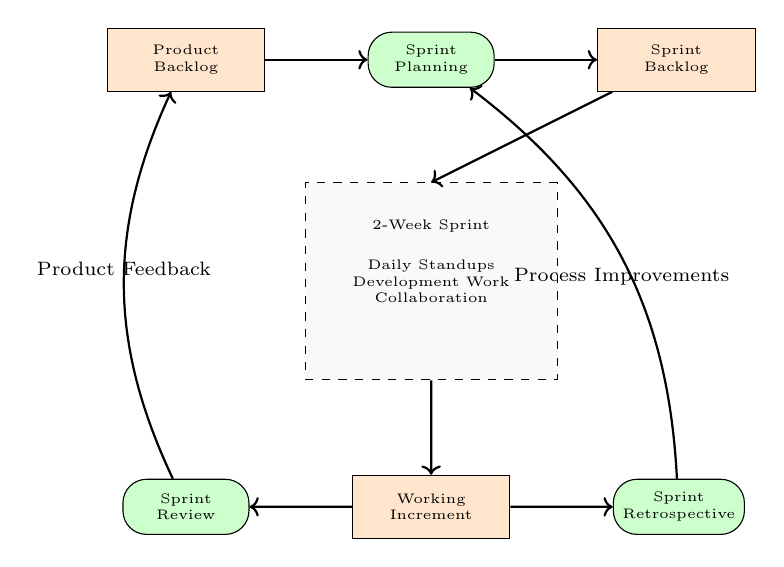
\begin{tikzpicture}[
scale=0.7,
artifact/.style={rectangle, draw, fill=orange!20, minimum height=0.8cm, minimum width=2cm, align=center, font=\tiny},
event/.style={rectangle, draw, fill=green!20, minimum height=0.7cm, minimum width=1.6cm, align=center, font=\tiny, rounded corners=0.3cm},
arrow/.style={->, thick},
sprint/.style={rectangle, draw, dashed, fill=gray!5, minimum height=2.5cm, minimum width=3.2cm}
]
% Top row - Planning phase
\node[artifact] (product_backlog) {Product\\Backlog};
\node[event, right=1.3cm of product_backlog] (sprint_planning) {Sprint\\Planning};
\node[artifact, right=1.3cm of sprint_planning] (sprint_backlog) {Sprint\\Backlog};
% Sprint box
\node[sprint, below=1.2cm of sprint_planning] (sprint_container) {};
\node[font=\bfseries, font=\tiny] at ([yshift=1cm]sprint_container.center) {2-Week Sprint};
\node[font=\tiny, align=center] at (sprint_container.center) {Daily Standups\\Development Work\\Collaboration};
% Bottom row - Review phase
\node[artifact, below=1.2cm of sprint_container] (increment) {Working\\Increment};
\node[event, left=1.3cm of increment] (sprint_review) {Sprint\\Review};
\node[event, right=1.3cm of increment] (retrospective) {Sprint\\Retrospective};
% Main flow arrows
\draw[arrow] (product_backlog) -- (sprint_planning);
\draw[arrow] (sprint_planning) -- (sprint_backlog);
\draw[arrow] (sprint_backlog) -- (sprint_container.north);
\draw[arrow] (sprint_container.south) -- (increment);
\draw[arrow] (increment) -- (sprint_review);
\draw[arrow] (increment) -- (retrospective);
% Feedback loops
\draw[arrow, bend left=25] (sprint_review) to node[above, font=\scriptsize] {Product Feedback} (product_backlog);
\draw[arrow, bend right=25] (retrospective) to node[below, font=\scriptsize] {Process Improvements} (sprint_planning);
\end{tikzpicture}
\caption{The Scrum Framework - Process Flow}
\label{fig:scrum_framework}
\end{figure}
\end{frame}

\begin{frame}{Project Management and Workflow Tools}
To support this Agile Scrum process, a specific set of digital tools was employed:
\begin{itemize}
\item \textbf{GitHub:} Used for version control and managing the \textbf{Product} and \textbf{Sprint Backlogs} via Projects and Issues features for tracking search engine development.
\item \textbf{Microsoft Teams:} Used for formal academic supervision meetings.
\item \textbf{Lark:} Serves as the central collaboration hub for daily communication, task tracking, and sprint management, coordinating distributed system components and data ingestion pipelines.
\end{itemize}
\end{frame}

\begin{frame}{Product Manager Interview - Requirements Discovery}
\scriptsize
\textbf{Example Q:} Can you describe the current challenges your technical teams face when searching for internal documentation?

\textbf{Outcome:}
\begin{itemize}
    \item Engineers spend 30-45 minutes daily searching across fragmented systems (Confluence, Google Drive, Git repositories, local shares).
    \item Existing keyword search misses conceptually related documents due to terminology variations.
    \item Critical visual information in charts and diagrams is not searchable, forcing manual document browsing.
    \item No unified interface, requiring context switching between multiple tools.
\end{itemize}

\vspace{0.5em}
\textbf{Example Q:} What types of queries do your teams typically need answers for?

\textbf{Outcome:}
\begin{itemize}
    \item Technical how-to questions requiring code examples and architecture diagrams.
    \item Troubleshooting queries needing logs, error messages, and past incident reports.
    \item Policy and compliance questions requiring exact citations from official documents.
    \item Comparative analysis requiring synthesis across multiple technical specifications.
    \item This revealed need for both precise retrieval and intelligent summarization.
\end{itemize}
\end{frame}

\begin{frame}{Product Manager Interview - Feature Priorities}
\scriptsize
\textbf{Example Q:} If you had to prioritize three capabilities for the search system, what would they be?

\textbf{Outcome:}
\begin{itemize}
    \item \textbf{Priority 1:} Multimodal search that can find documents based on visual content descriptions, not just text.
    \item \textbf{Priority 2:} Conversational interface where follow up questions refine results without starting over.
    \item \textbf{Priority 3:} Source attribution with exact citations so answers can be verified and trusted.
    \item Additional need: Sub-second query response time for daily usage adoption.
\end{itemize}

\vspace{0.5em}
\textbf{Example Q:} How do you currently evaluate whether search results are relevant?

\textbf{Outcome:}
\begin{itemize}
    \item Manual inspection of top 10 results for precision.
    \item User feedback on whether they found what they needed.
    \item Time to complete search task as efficiency metric.
    \item This informed our evaluation methodology using NDCG@10, MRR, and latency measurements.
\end{itemize}
\end{frame}

\begin{frame}{Workflow Analysis}
Detailed observations of Infinity Datatech manual search processes were conducted:
\begin{itemize}
    \item \textbf{Process mapping:} Documented the end to end workflow from query formulation to answer discovery, revealing an average of 7 context switches per search session across different data sources.
    \item \textbf{Time motion studies:} Measured time spent on manual tasks to identify bottlenecks. Average search session: 12 minutes, with 60 percent spent navigating between systems rather than evaluating content.
    \item \textbf{Artifact analysis:} Examined search logs and user feedback to understand information needs. Found 40 percent of queries require visual evidence and 65 percent benefit from conversational refinement.
    \item \textbf{Tool evaluation:} Assessed the current toolset (Confluence search, Google Drive search, file system grep) to find gaps. No system provided multimodal retrieval or intelligent ranking beyond keyword matching.
\end{itemize}
\end{frame}

\begin{frame}{Hierarchical Task Analysis}
The Hierarchical Task Analysis below outlines the system functional structure, decomposed into eight primary modules. This task breakdown forms the basis for the use cases and activity diagrams that follow.

\vspace{0.5em}
\begin{figure}
    \centering
    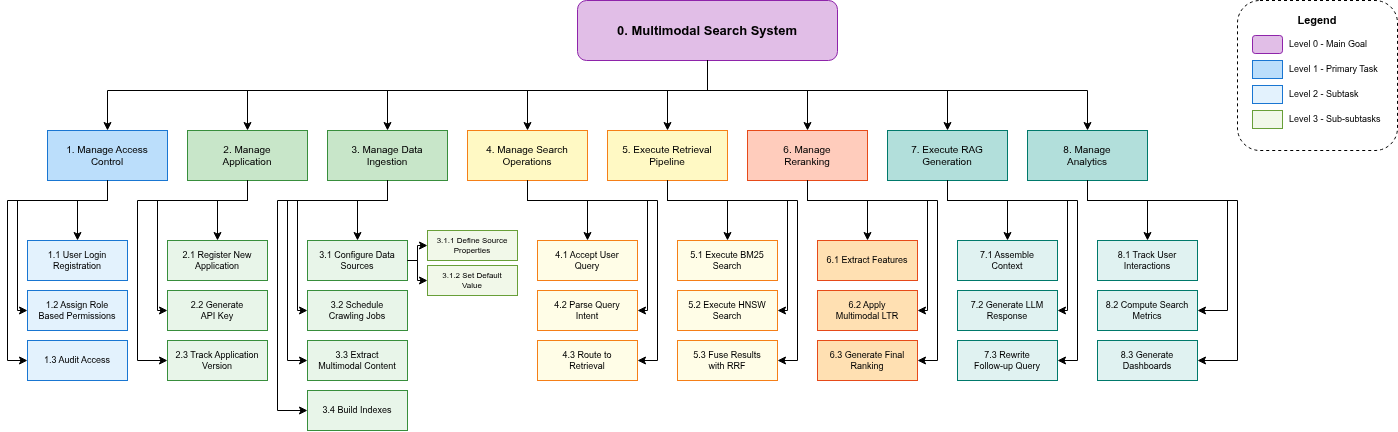
\includegraphics[width=0.95\textwidth]{HTA.drawio.png}
    \caption{Hierarchical Task Analysis of Verdant Search System}
    \label{fig:hta}
\end{figure}
\end{frame}

\begin{frame}{Stakeholder Introduction}
    \begin{columns}[t]
        \column{.48\textwidth}
        \textbf{Infinity Data Tech Sdn. Bhd.}
        \begin{itemize}
            \item Malaysian company specializing in VPN and AI customer service products
            \item Own application products and in house development
            \item Focus on software development and network protocol research
        \end{itemize}
        
        \column{.48\textwidth}
        \textbf{Project Context}
        \begin{itemize}
            \item Internal knowledge base search for technical teams
            \item Customer support documentation retrieval
            \item VPN technical knowledge and censorship circumvention expertise
        \end{itemize}
    \end{columns}
\end{frame}

\begin{frame}{System Architecture Overview}
    \begin{columns}[t]
        \column{.48\textwidth}
        \textbf{Backend Pipeline}
        \begin{itemize}
            \item Distributed web crawling with text and image extraction
            \item Dual indexing: Inverted index (BM25) + HNSW (CLIP embeddings)
            \item Compressed storage with incremental updates
            \item Two stage ranking: Fast retrieval + Multimodal LTR reranking
        \end{itemize}
        
        \column{.48\textwidth}
        \textbf{Frontend Interface}
        \begin{itemize}
            \item Dual panel UI: Document list + AI chat
            \item Conversational query refinement
            \item Real time result updates
            \item Closed loop: User follow up leads to query rewriting leads to new retrieval leads to updated AI response
        \end{itemize}
    \end{columns}
\end{frame}


%------------------------------------------------
\section{Requirements Specification}
%------------------------------------------------

\begin{frame}{Project Modules Overview}
    \footnotesize
    \begin{table}
        \centering
        \renewcommand{\arraystretch}{1.15}
        \begin{tabular}{p{0.18\textwidth}|p{0.72\textwidth}}
        \toprule
        \textbf{Module Name} & \textbf{Description} \\
        \midrule
        \textbf{Module 1:} User Management & User authentication, authorization, and profile management with SSO integration. \\
        \midrule
        \textbf{Module 2:} Search and Retrieval & Hybrid search (BM25 + HNSW vector) with multimodal reranking. \\
        \midrule
        \textbf{Module 3:} Data Ingestion & Distributed crawling, document processing, chunking, and index building. \\
        \midrule
        \textbf{Module 4:} Analytics and Monitoring & System metrics, search analytics, and performance monitoring. \\
        \midrule
        \textbf{Module 5:} RAG Generation & LLM-based answer generation with context injection and citations. \\
        \bottomrule
        \end{tabular}
    \end{table}
\end{frame}

\begin{frame}{Functional Requirements: Module 1 User Management}
    \tiny
    \renewcommand{\arraystretch}{0.68}
    \begin{table}
        \centering
        \begin{tabular}{p{0.10\textwidth}|p{0.08\textwidth}|p{0.54\textwidth}|p{0.12\textwidth}}
        \toprule
        \textbf{UC ID} & \textbf{FR ID} & \textbf{Functional Requirements} & \textbf{Priority} \\
        \midrule
        \multirow{3}{*}{UC-01} & FR-1.1 & User shall register an account with email and password. & High \\
        & FR-1.2 & System shall validate email format and password strength. & High \\
        & FR-1.3 & System shall send verification email upon registration. & Medium \\
        \midrule
        \multirow{2}{*}{UC-02, UC-03} & FR-1.4 & User shall login with email/password or SSO authentication. & High \\
        & FR-1.5 & System shall support SSO providers (LDAP, Okta, Azure AD). & High \\
        \midrule
        UC-07 & FR-1.6 & System shall authenticate user credentials securely. & High \\
        \midrule
        \multirow{2}{*}{UC-04} & FR-1.7 & User shall manage profile with configurable preferences. & Medium \\
        & FR-1.8 & User shall update display name, avatar, and notification settings. & Medium \\
        \midrule
        UC-08 & FR-1.9 & User shall configure language and search settings. & Medium \\
        \midrule
        \multirow{3}{*}{UC-05} & FR-1.10 & User shall view and manage their chat history. & Medium \\
        & FR-1.11 & System shall display chat history with timestamps and summaries. & Medium \\
        & FR-1.12 & User shall export chat history in JSON or markdown format. & Low \\
        \midrule
        UC-09 & FR-1.13 & System shall provide search functionality within chat history. & Medium \\
        \midrule
        UC-11 & FR-1.14 & User shall be able to delete individual or bulk chat entries. & Medium \\
        \midrule
        \multirow{2}{*}{UC-06} & FR-1.15 & System shall implement session management with timeout. & Medium \\
        & FR-1.16 & System shall automatically logout after 24 hours of inactivity. & Medium \\
        \midrule
        UC-10 & FR-1.17 & System shall validate session tokens on each request. & Medium \\
        \bottomrule
        \end{tabular}
    \end{table}
\end{frame}

\begin{frame}{Functional Requirements: Module 2 Search and Retrieval (1/2)}
    \tiny
    \renewcommand{\arraystretch}{0.65}
    \begin{table}
        \centering
        \begin{tabular}{p{0.12\textwidth}|p{0.08\textwidth}|p{0.52\textwidth}|p{0.12\textwidth}}
        \toprule
        \textbf{UC ID} & \textbf{FR ID} & \textbf{Functional Requirements} & \textbf{Priority} \\
        \midrule
        \multirow{3}{*}{UC-12} & FR-2.1 & User shall submit search query through text input. & High \\
        & FR-2.2 & System shall sanitize and normalize query text. & High \\
        & FR-2.3 & System shall support query expansion with synonyms. & Medium \\
        \midrule
        \multirow{2}{*}{UC-16} & FR-2.4 & System shall perform keyword search using BM25. & High \\
        & FR-2.5 & System shall build inverted index with term posting lists. & High \\
        \midrule
        \multirow{2}{*}{UC-17} & FR-2.6 & System shall perform vector search using HNSW. & High \\
        & FR-2.7 & System shall encode queries with Sentence-BERT embeddings. & High \\
        \midrule
        \multirow{2}{*}{UC-18} & FR-2.8 & System shall support hybrid search with RRF fusion. & High \\
        & FR-2.9 & System shall combine BM25 and vector scores with weighted fusion. & High \\
        \midrule
        UC-22 & FR-2.10 & System shall support pre-filtering on metadata fields. & Medium \\
        \bottomrule
        \end{tabular}
    \end{table}
\end{frame}

\begin{frame}{Functional Requirements: Module 2 Search and Retrieval (2/2)}
    \tiny
    \renewcommand{\arraystretch}{0.68}
    \begin{table}
        \centering
        \begin{tabular}{p{0.12\textwidth}|p{0.08\textwidth}|p{0.52\textwidth}|p{0.12\textwidth}}
        \toprule
        \textbf{UC ID} & \textbf{FR ID} & \textbf{Functional Requirements} & \textbf{Priority} \\
        \midrule
        \multirow{2}{*}{UC-13} & FR-2.11 & System shall display search results as ranked document list. & High \\
        & FR-2.12 & System shall show document snippets with highlighted keywords. & High \\
        \midrule
        UC-19 & FR-2.13 & System shall return ranked list of context chunks. & High \\
        \midrule
        \multirow{2}{*}{UC-20} & FR-2.14 & System shall apply multimodal reranking to top candidates. & High \\
        & FR-2.15 & System shall use BLIP-2 for cross-modal relevance scoring. & High \\
        \midrule
        \multirow{2}{*}{UC-21} & FR-2.16 & System shall extract and attach metadata to chunks. & Medium \\
        & FR-2.17 & Metadata shall include filename, page number, and timestamp. & Medium \\
        \midrule
        \multirow{2}{*}{UC-14} & FR-2.18 & User shall ask follow-up questions to refine results. & High \\
        & FR-2.19 & System shall track conversation history for context. & High \\
        \midrule
        UC-23 & FR-2.20 & System shall rewrite follow-ups into standalone queries. & High \\
        \midrule
        UC-24 & FR-2.21 & System shall maintain conversation context across turns. & High \\
        \midrule
        UC-15 & FR-2.22 & User shall filter results by metadata fields. & Medium \\
        \bottomrule
        \end{tabular}
    \end{table}
\end{frame}

\begin{frame}{Functional Requirements: Module 3 Data Ingestion (1/2)}
    \tiny
    \renewcommand{\arraystretch}{0.62}
    \begin{table}
        \centering
        \begin{tabular}{p{0.14\textwidth}|p{0.08\textwidth}|p{0.50\textwidth}|p{0.12\textwidth}}
        \toprule
        \textbf{UC ID} & \textbf{FR ID} & \textbf{Functional Requirements} & \textbf{Priority} \\
        \midrule
        \multirow{2}{*}{UC-25} & FR-3.1 & Administrator shall configure data ingestion sources. & High \\
        & FR-3.2 & System shall validate source credentials and permissions. & High \\
        \midrule
        \multirow{3}{*}{UC-26} & FR-3.3 & System shall trigger distributed crawling jobs. & High \\
        & FR-3.4 & System shall use Kafka for job coordination and task distribution. & High \\
        & FR-3.5 & System shall implement exponential backoff for failed crawls. & Medium \\
        \midrule
        \multirow{2}{*}{UC-29} & FR-3.6 & System shall crawl Confluence spaces via REST API. & High \\
        & FR-3.7 & System shall respect Confluence rate limits and pagination. & High \\
        \midrule
        \multirow{2}{*}{UC-30} & FR-3.8 & System shall crawl Google Drive files via Drive API. & High \\
        & FR-3.9 & System shall handle Google Docs, Sheets, Slides formats. & High \\
        \midrule
        UC-31 & FR-3.10 & System shall crawl Git repositories via Git protocol. & High \\
        \midrule
        UC-32 & FR-3.11 & System shall crawl local network shares via SMB/NFS. & High \\
        \midrule
        \multirow{3}{*}{UC-33} & FR-3.12 & System shall extract text and images from documents. & High \\
        & FR-3.13 & System shall use OCR for scanned PDF content. & Medium \\
        & FR-3.14 & System shall extract images with captions from documents. & High \\
        \bottomrule
        \end{tabular}
    \end{table}
\end{frame}

\begin{frame}{Functional Requirements: Module 3 Data Ingestion (2/2)}
    \tiny
    \renewcommand{\arraystretch}{0.64}
    \begin{table}
        \centering
        \begin{tabular}{p{0.14\textwidth}|p{0.08\textwidth}|p{0.50\textwidth}|p{0.12\textwidth}}
        \toprule
        \textbf{UC ID} & \textbf{FR ID} & \textbf{Functional Requirements} & \textbf{Priority} \\
        \midrule
        \multirow{2}{*}{UC-34} & FR-3.15 & System shall chunk documents into semantic segments. & High \\
        & FR-3.16 & System shall maintain chunk overlap for context preservation. & High \\
        \midrule
        UC-38 & FR-3.17 & System shall support chunking by heading structure. & Medium \\
        \midrule
        UC-39 & FR-3.18 & System shall support chunking by paragraph boundaries. & Medium \\
        \midrule
        UC-40 & FR-3.19 & System shall support fixed token count chunking. & Medium \\
        \midrule
        \multirow{2}{*}{UC-35} & FR-3.20 & System shall build inverted index for BM25. & High \\
        & FR-3.21 & System shall use Pyserini for efficient index construction. & High \\
        \midrule
        \multirow{2}{*}{UC-36} & FR-3.22 & System shall build HNSW vector index. & High \\
        & FR-3.23 & System shall use FAISS for scalable vector indexing. & High \\
        \midrule
        \multirow{2}{*}{UC-37} & FR-3.24 & System shall generate dense vector embeddings. & High \\
        & FR-3.25 & System shall use CLIP for image embeddings. & High \\
        \midrule
        UC-27 & FR-3.26 & Administrator shall monitor indexing progress. & Medium \\
        \midrule
        \multirow{2}{*}{UC-28} & FR-3.27 & Administrator shall manage index refresh schedule. & Medium \\
        & FR-3.28 & System shall support cron-based scheduling. & Medium \\
        \midrule
        UC-41 & FR-3.29 & System shall support real-time sync with webhooks. & Medium \\
        \midrule
        UC-42 & FR-3.30 & System shall support scheduled batch updates. & High \\
        \bottomrule
        \end{tabular}
    \end{table}
\end{frame}

\begin{frame}{Functional Requirements: Module 5 RAG Generation (1/2)}
    \tiny
    \renewcommand{\arraystretch}{0.63}
    \begin{table}
        \centering
        \begin{tabular}{p{0.14\textwidth}|p{0.08\textwidth}|p{0.50\textwidth}|p{0.12\textwidth}}
        \toprule
        \textbf{UC ID} & \textbf{FR ID} & \textbf{Functional Requirements} & \textbf{Priority} \\
        \midrule
        \multirow{2}{*}{UC-43} & FR-5.1 & System shall receive and process user query. & High \\
        & FR-5.2 & System shall validate query length and format. & High \\
        \midrule
        \multirow{2}{*}{UC-47} & FR-5.3 & System shall inject retrieved context into LLM prompt. & High \\
        & FR-5.4 & System shall format context with document metadata. & High \\
        \midrule
        \multirow{2}{*}{UC-44} & FR-5.5 & User shall view AI generated answer based on context. & High \\
        & FR-5.6 & System shall display answer with markdown formatting. & High \\
        \midrule
        \multirow{2}{*}{UC-51} & FR-5.7 & LLM shall generate answers grounded in context. & High \\
        & FR-5.8 & LLM shall avoid hallucination by using only retrieved content. & High \\
        \midrule
        \multirow{2}{*}{UC-52} & FR-5.9 & System shall add inline citations to answers. & High \\
        & FR-5.10 & Citations shall link to source document and page number. & High \\
        \midrule
        UC-53 & FR-5.11 & System shall validate answer grounding with entailment check. & Medium \\
        \midrule
        UC-54 & FR-5.12 & System shall indicate knowledge base limitations clearly. & High \\
        \midrule
        \multirow{2}{*}{UC-48} & FR-5.13 & System shall stream LLM response in real-time. & High \\
        & FR-5.14 & System shall use server-sent events for streaming. & High \\
        \bottomrule
        \end{tabular}
    \end{table}
\end{frame}

\begin{frame}{Functional Requirements: Module 5 RAG Generation (2/2)}
    \tiny
    \renewcommand{\arraystretch}{0.66}
    \begin{table}
        \centering
        \begin{tabular}{p{0.14\textwidth}|p{0.08\textwidth}|p{0.50\textwidth}|p{0.12\textwidth}}
        \toprule
        \textbf{UC ID} & \textbf{FR ID} & \textbf{Functional Requirements} & \textbf{Priority} \\
        \midrule
        \multirow{2}{*}{UC-45} & FR-5.15 & User shall ask follow-up questions. & High \\
        & FR-5.16 & System shall detect follow-up vs new query intent. & High \\
        \midrule
        \multirow{2}{*}{UC-49} & FR-5.17 & System shall maintain conversation history. & High \\
        & FR-5.18 & System shall limit history to last 10 conversation turns. & Medium \\
        \midrule
        \multirow{2}{*}{UC-55} & FR-5.19 & System shall rewrite follow-ups with context. & High \\
        & FR-5.20 & System shall use LLM for query rewriting with history. & High \\
        \midrule
        UC-56 & FR-5.21 & System shall trigger new retrieval after query rewriting. & High \\
        \midrule
        UC-59 & FR-5.22 & System shall update document list with new results. & High \\
        \midrule
        UC-57 & FR-5.23 & System shall analyze user feedback on answers. & Medium \\
        \midrule
        UC-58 & FR-5.24 & System shall refine search strategy based on feedback. & Medium \\
        \midrule
        \multirow{2}{*}{UC-46} & FR-5.25 & User shall view source citations. & High \\
        & FR-5.26 & System shall highlight cited text in source documents. & Medium \\
        \midrule
        \multirow{2}{*}{UC-50} & FR-5.27 & System shall format source references. & Medium \\
        & FR-5.28 & References shall include title, author, and timestamp. & Medium \\
        \bottomrule
        \end{tabular}
    \end{table}
\end{frame}

\begin{frame}{Non Functional Requirements}
    \tiny
    \renewcommand{\arraystretch}{0.70}
    \begin{table}
        \centering
        \begin{tabular}{p{0.08\textwidth}|p{0.12\textwidth}|p{0.32\textwidth}|p{0.20\textwidth}|p{0.18\textwidth}}
        \toprule
        \textbf{Req ID} & \textbf{Quality Attribute} & \textbf{Requirement Description} & \textbf{How to Achieve} & \textbf{How to Verify} \\
        \midrule
        NFR 1.1 & Security: Authenticity & System shall integrate with internal identity providers. & LDAP/SAML/OAuth2 with JWT & SSO login testing \\
        \midrule
        NFR 1.2 & Security: Confidentiality & Results shall adhere to file permissions; access validated. & ACL enforcement at retrieval & Access audit logs \\
        \midrule
        NFR 1.3 & Security: Integrity & All data in private infrastructure; LLM self-hosted. & On-premise + AES-256 encryption & Security audit \\
        \midrule
        NFR 2.1 & Performance: Time & P90 latency under 4 seconds from query to response. & Two-stage ranking + Redis cache & Prometheus monitoring \\
        \midrule
        NFR 2.2 & Performance: Capacity & System scales to 10 million document index. & Distributed HNSW + Kafka sharding & Load test with 10M docs \\
        \midrule
        NFR 3.1 & Reliability: Fault Tolerance & System implements error handling and logging. & Circuit breakers + retry + ELK logs & Chaos engineering tests \\
        \midrule
        NFR 4.1 & Maintainability: Modularity & Components independently deployable. & Microservices + Docker + K8s & Deployment isolation tests \\
        \midrule
        NFR 5.1 & Usability: Learnability & New users complete basic search within 5 minutes. & Intuitive UI + help tooltips & User testing (n=10+) \\
        \bottomrule
        \end{tabular}
    \end{table}
\end{frame}

%------------------------------------------------
\section{System Analysis and Design}
%------------------------------------------------

\begin{frame}{System Analysis and Design - Use Case Diagram}
    \begin{figure}
        \centering
        \vspace{-3px}
        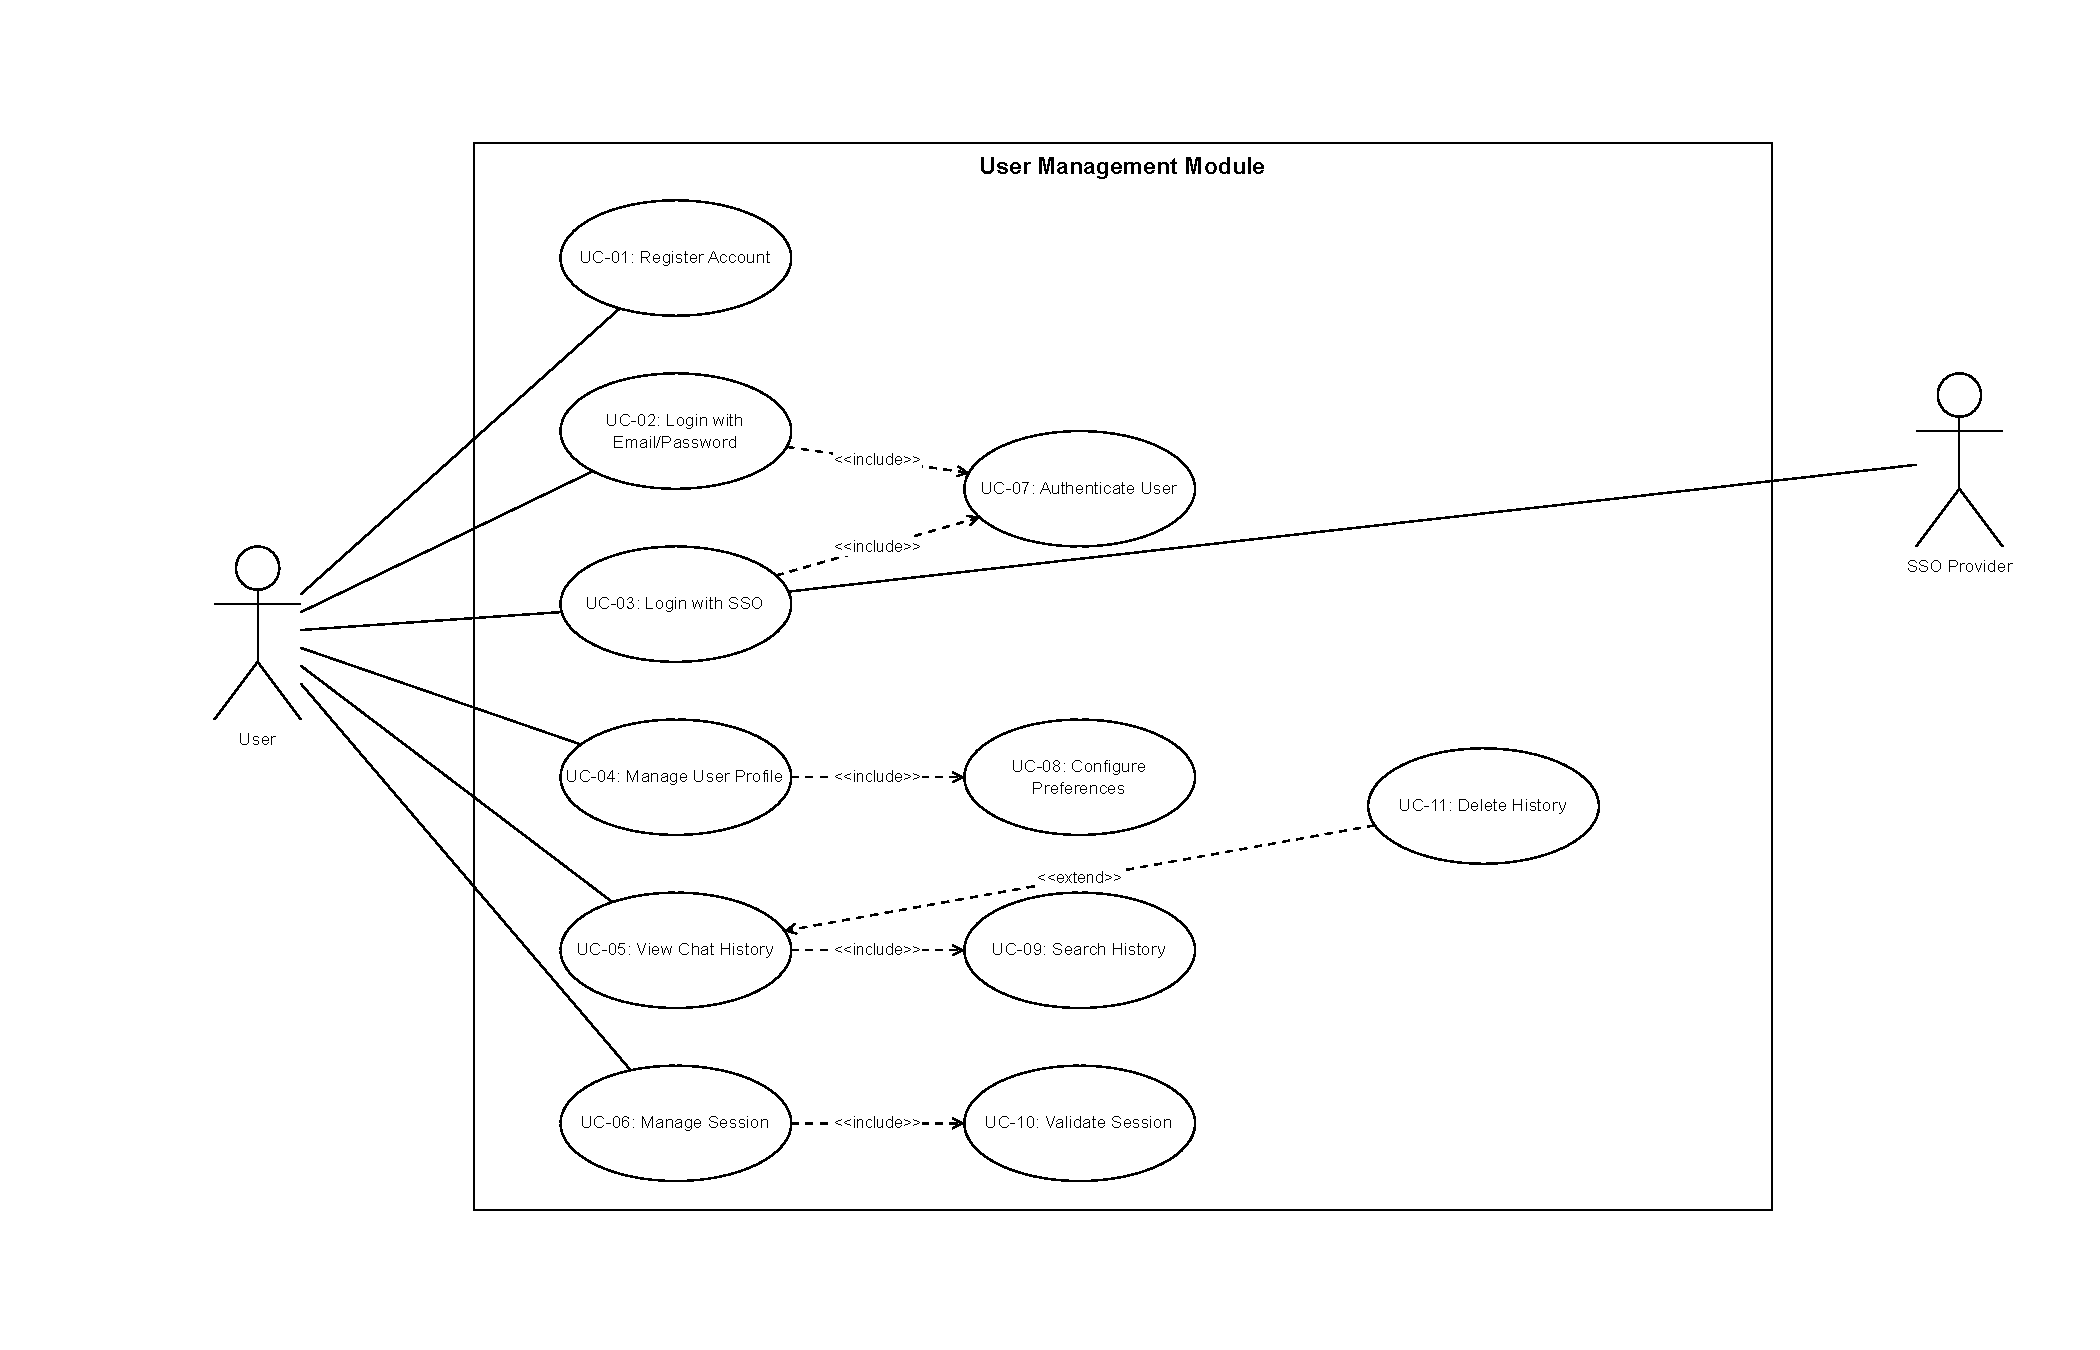
\includegraphics[width=0.90\linewidth]{updated_uc1.drawio.pdf}
        \label{fig:placeholder}
    \end{figure}
\end{frame}

\begin{frame}{System Analysis and Design - Use Case Diagram}
    \begin{figure}
        \centering
        \vspace{-3px}
        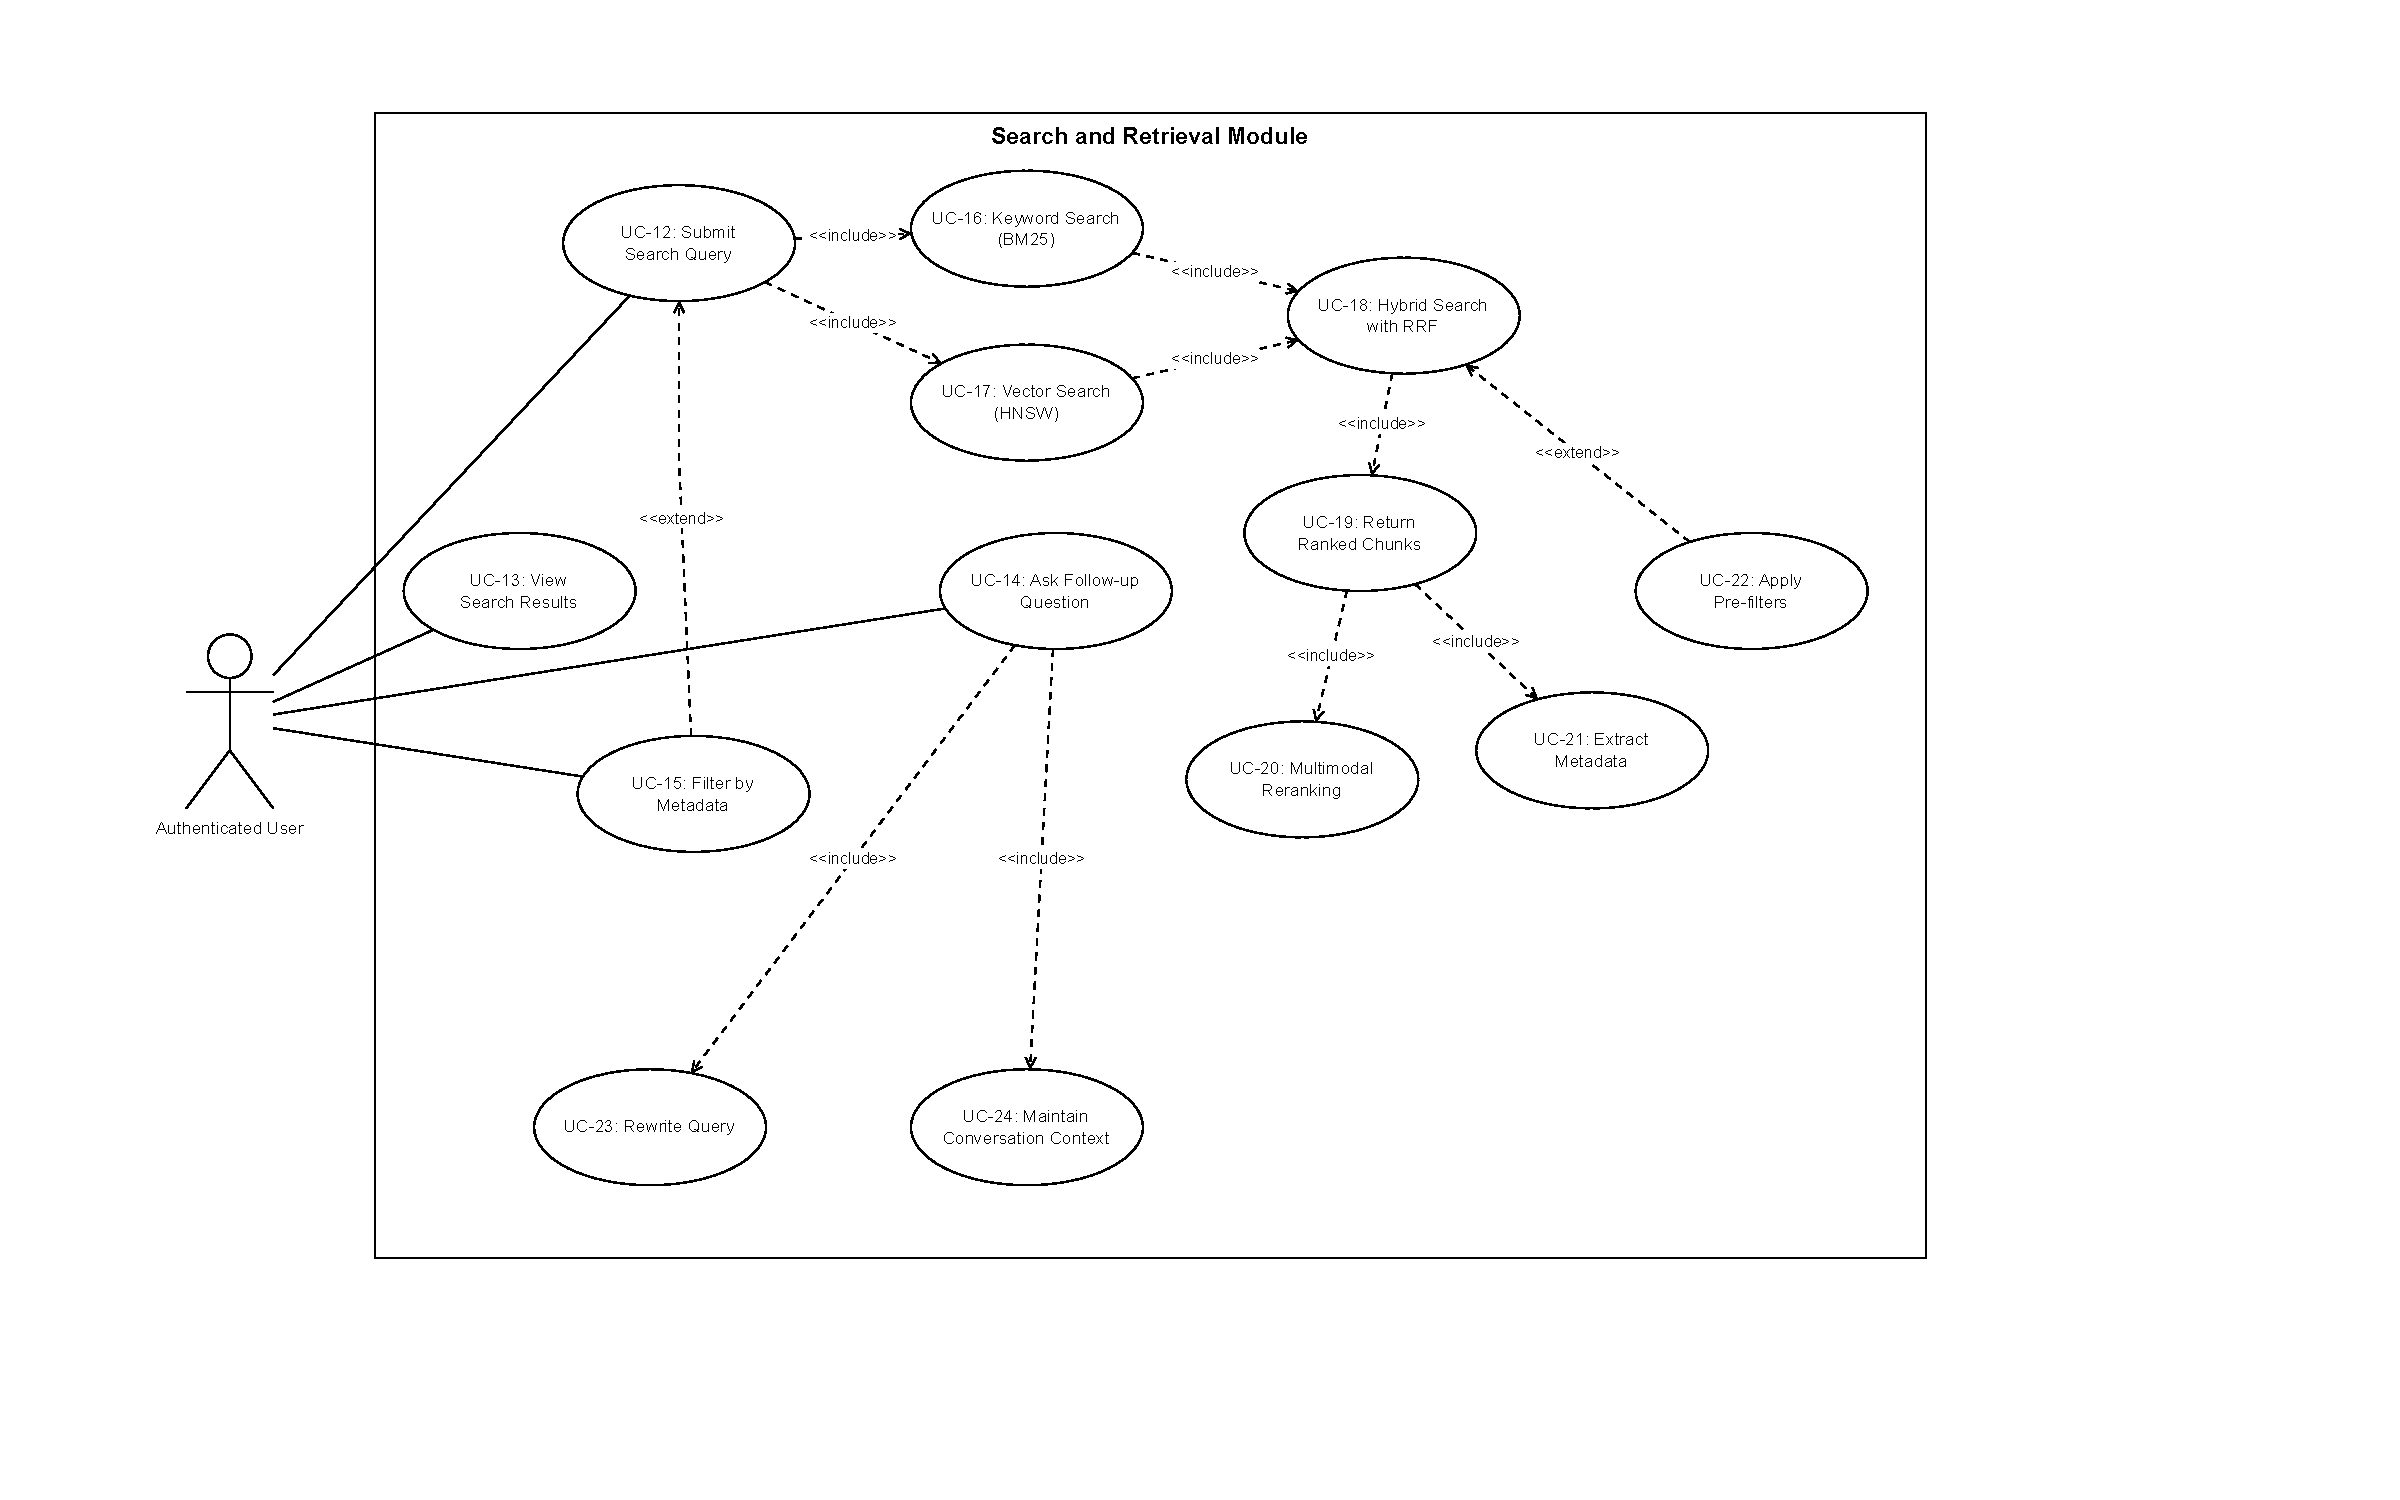
\includegraphics[width=0.90\linewidth]{updated_uc2.drawio.pdf}
        \label{fig:placeholder}
    \end{figure}
\end{frame}

\begin{frame}{System Analysis and Design - Use Case Diagram}
    \begin{figure}
        \centering
        \vspace{-6px}
        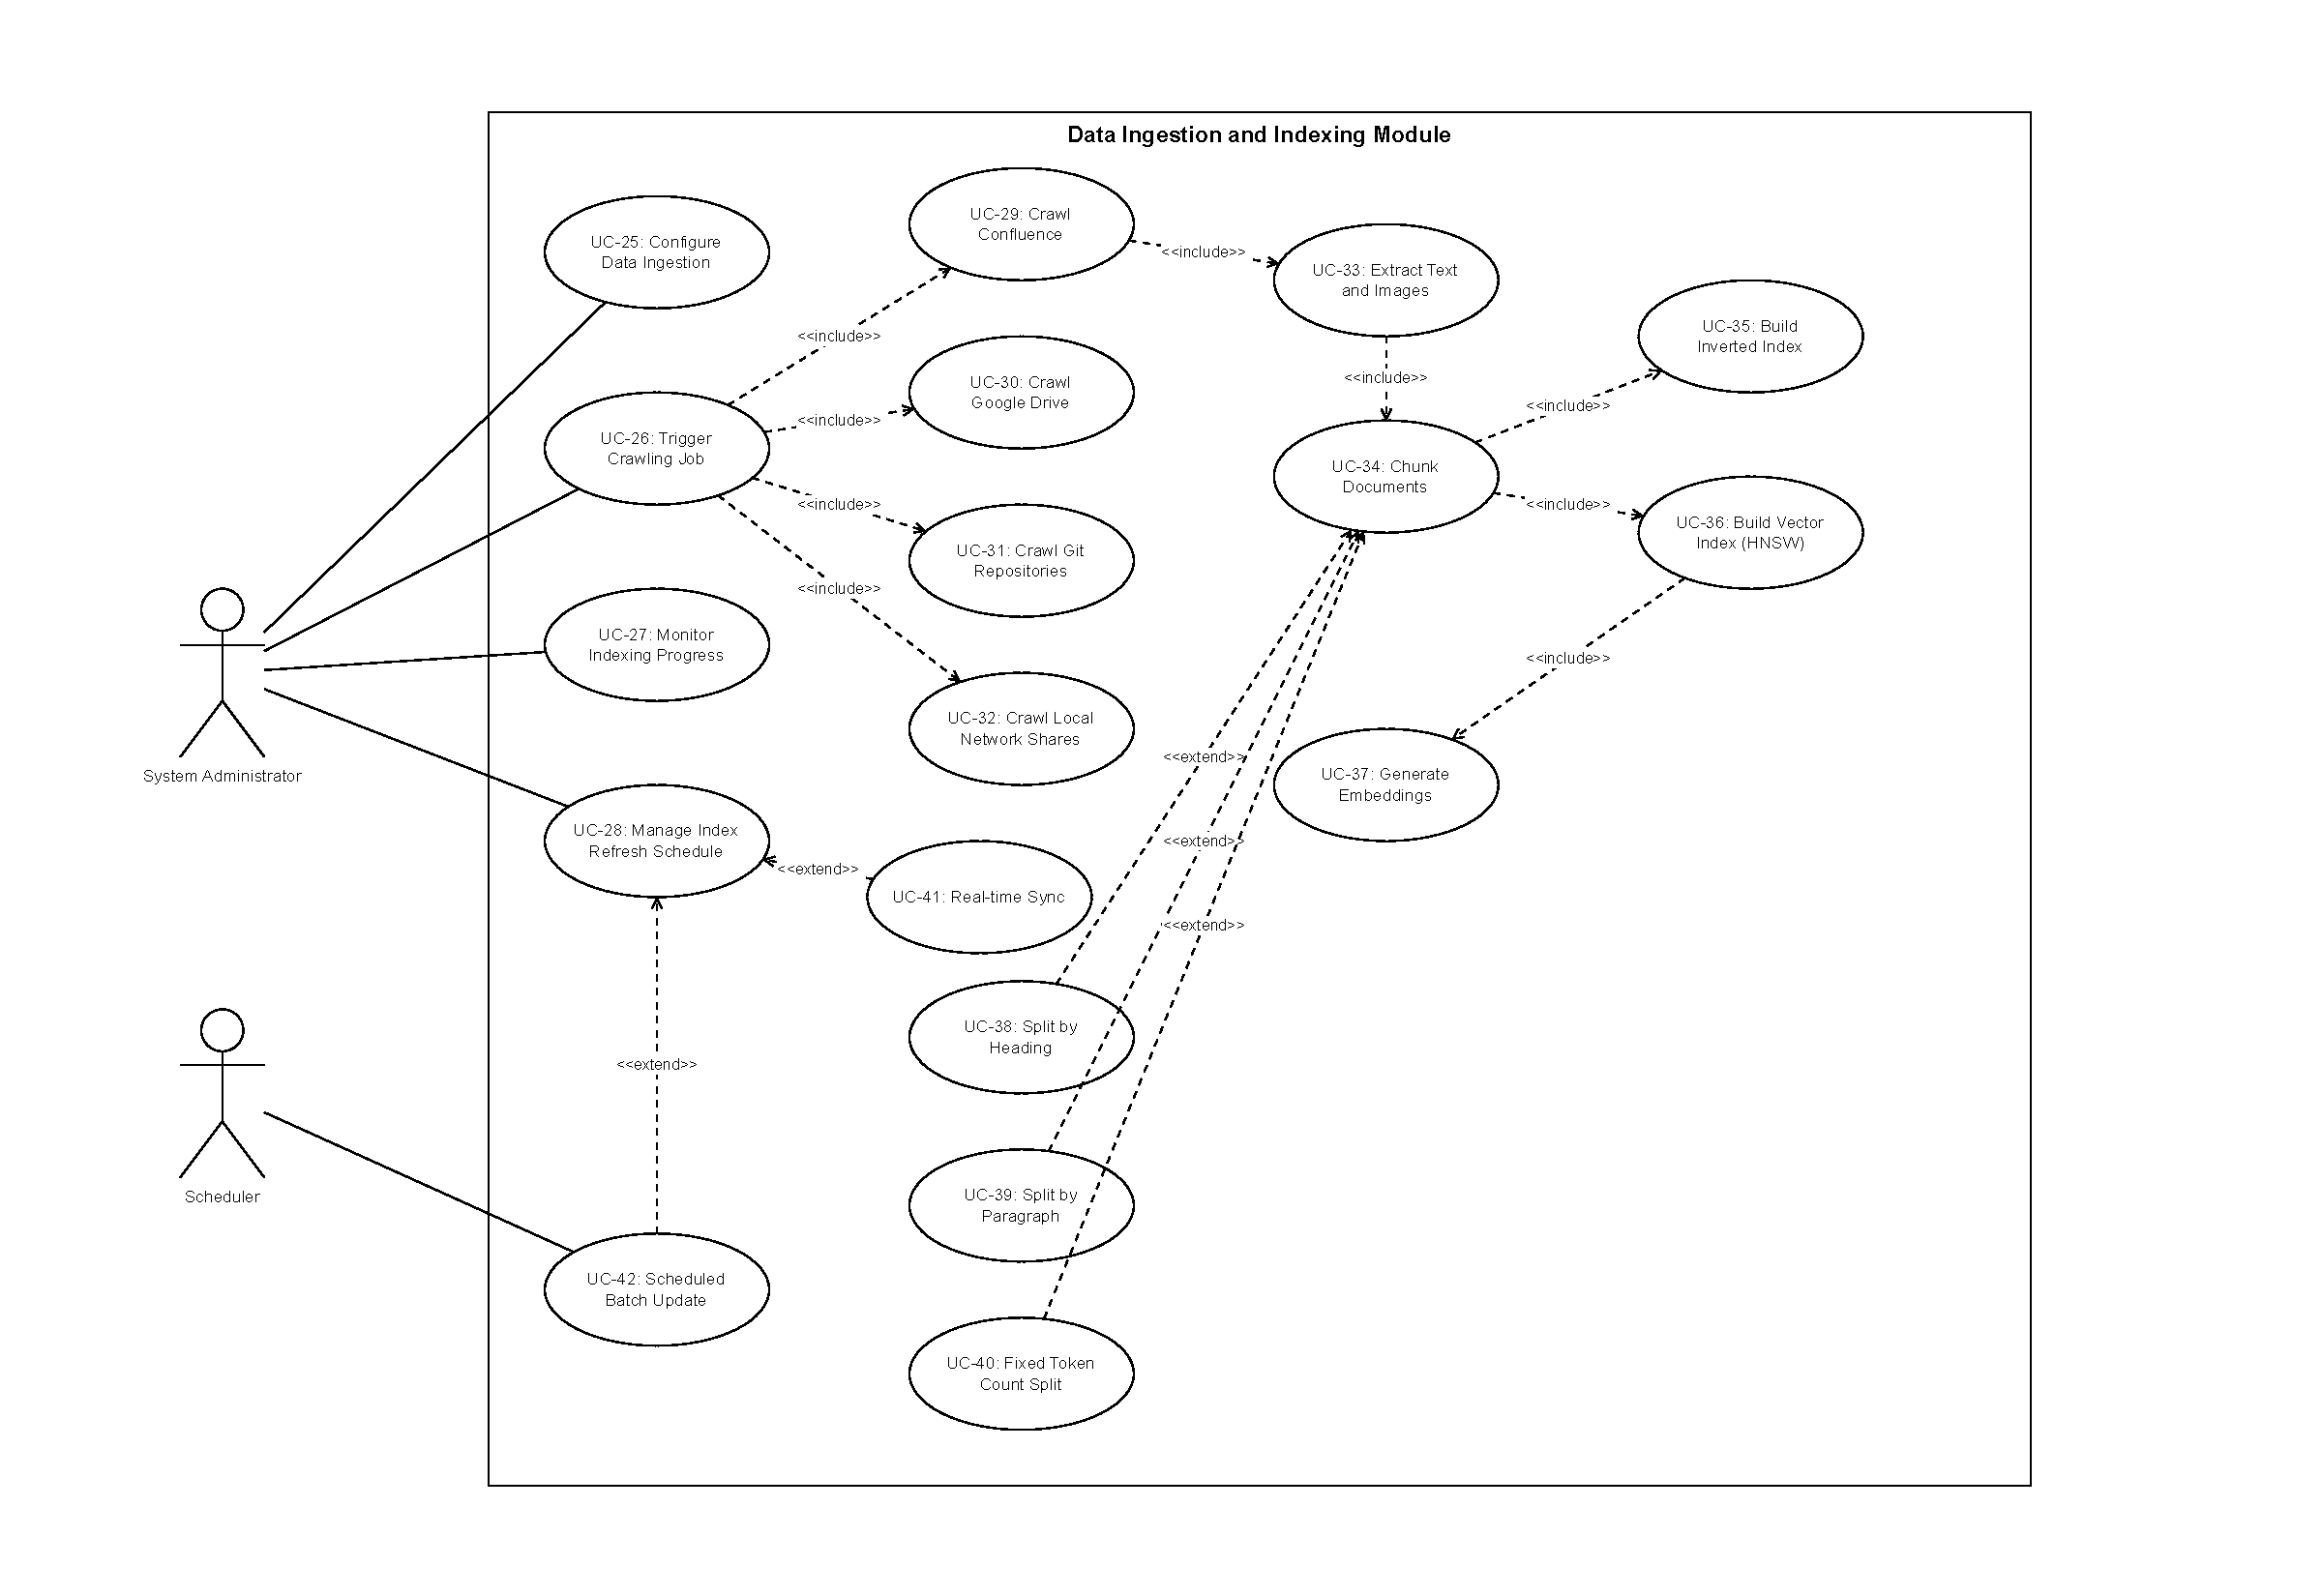
\includegraphics[width=0.86\linewidth]{updated_uc3.drawio.pdf}
        \label{fig:placeholder}
    \end{figure}
\end{frame}

\begin{frame}{System Analysis and Design - Use Case Diagram}
    \begin{figure}
        \centering
        \vspace{-3px}
        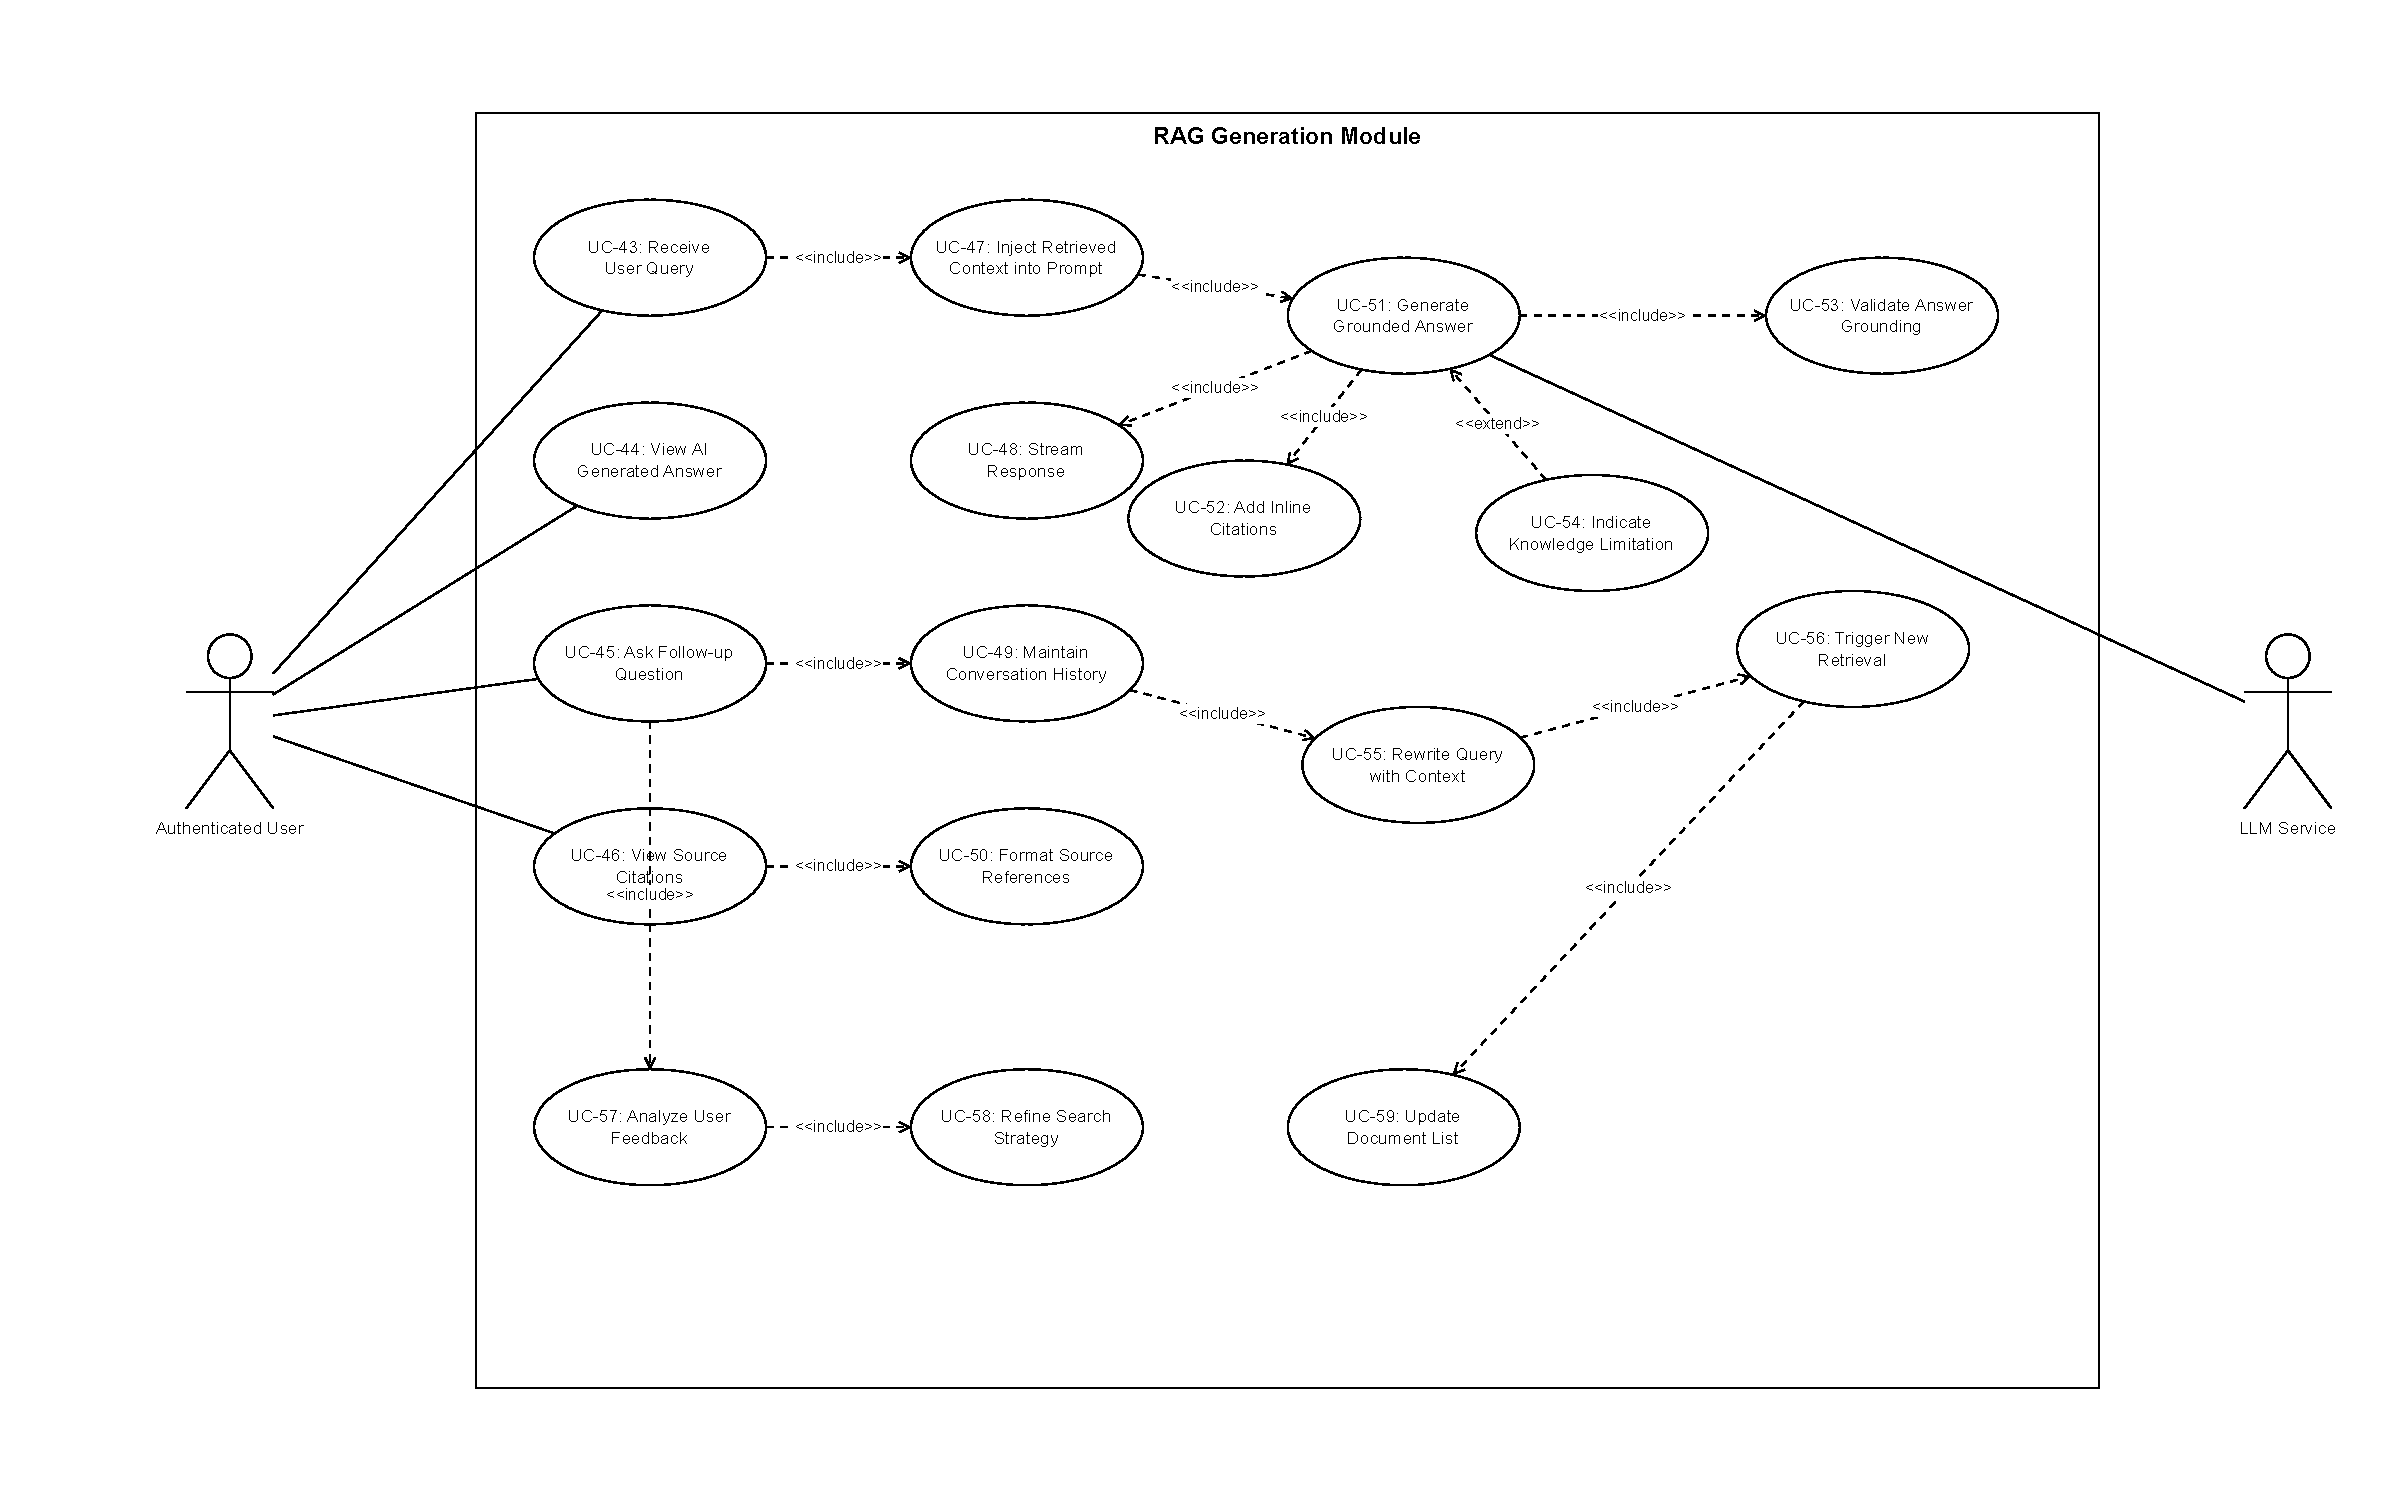
\includegraphics[width=0.90\linewidth]{updated_uc4.drawio.pdf}
        \label{fig:placeholder}
    \end{figure}
\end{frame}

\begin{frame}{System Analysis and Design - Activity Diagram}
    \begin{figure}
        \centering
        \vspace{-3px}
        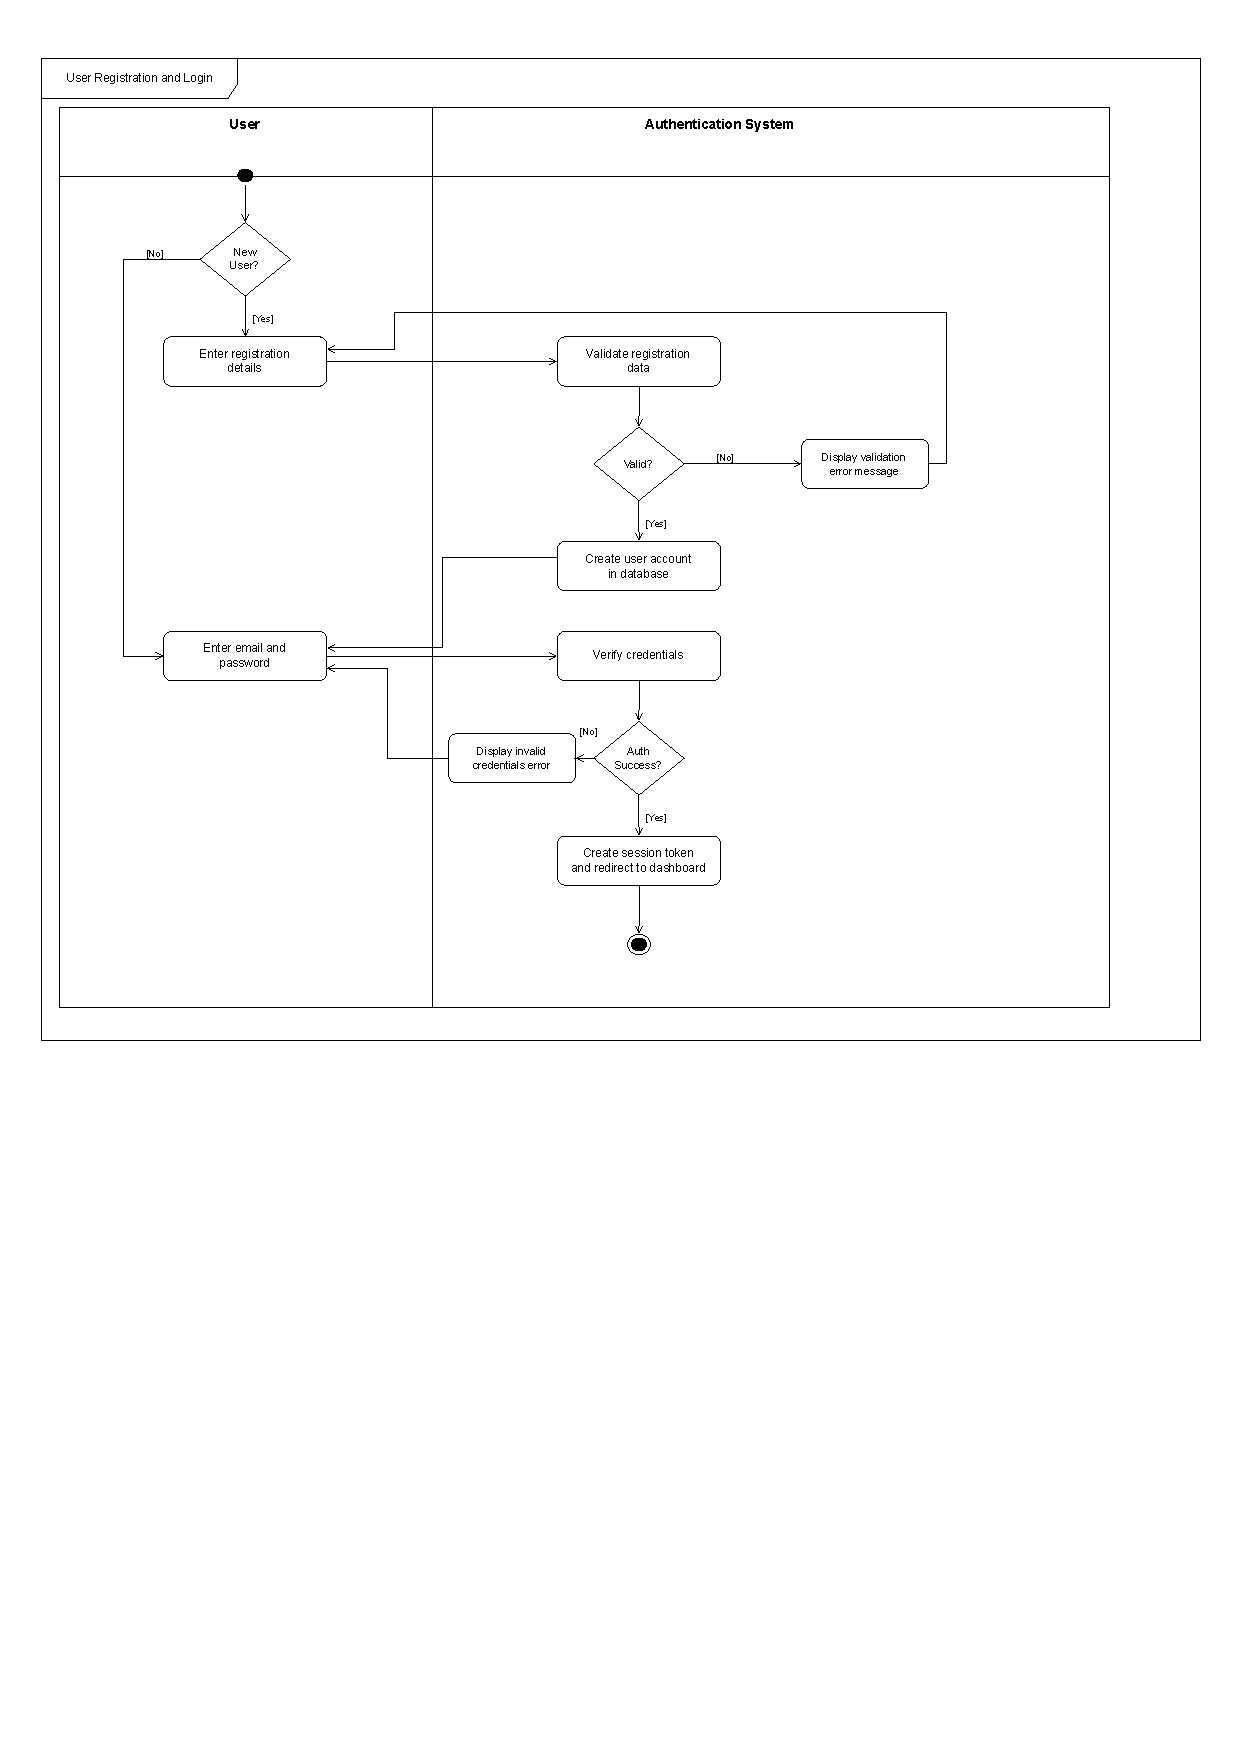
\includegraphics[width=0.55\linewidth]{activity1_fixed.drawio (3).pdf}
        \label{fig:placeholder}
    \end{figure}
\end{frame}

\begin{frame}{System Analysis and Design - Activity Diagram}
    \begin{figure}
        \centering
        \vspace{-3px}
        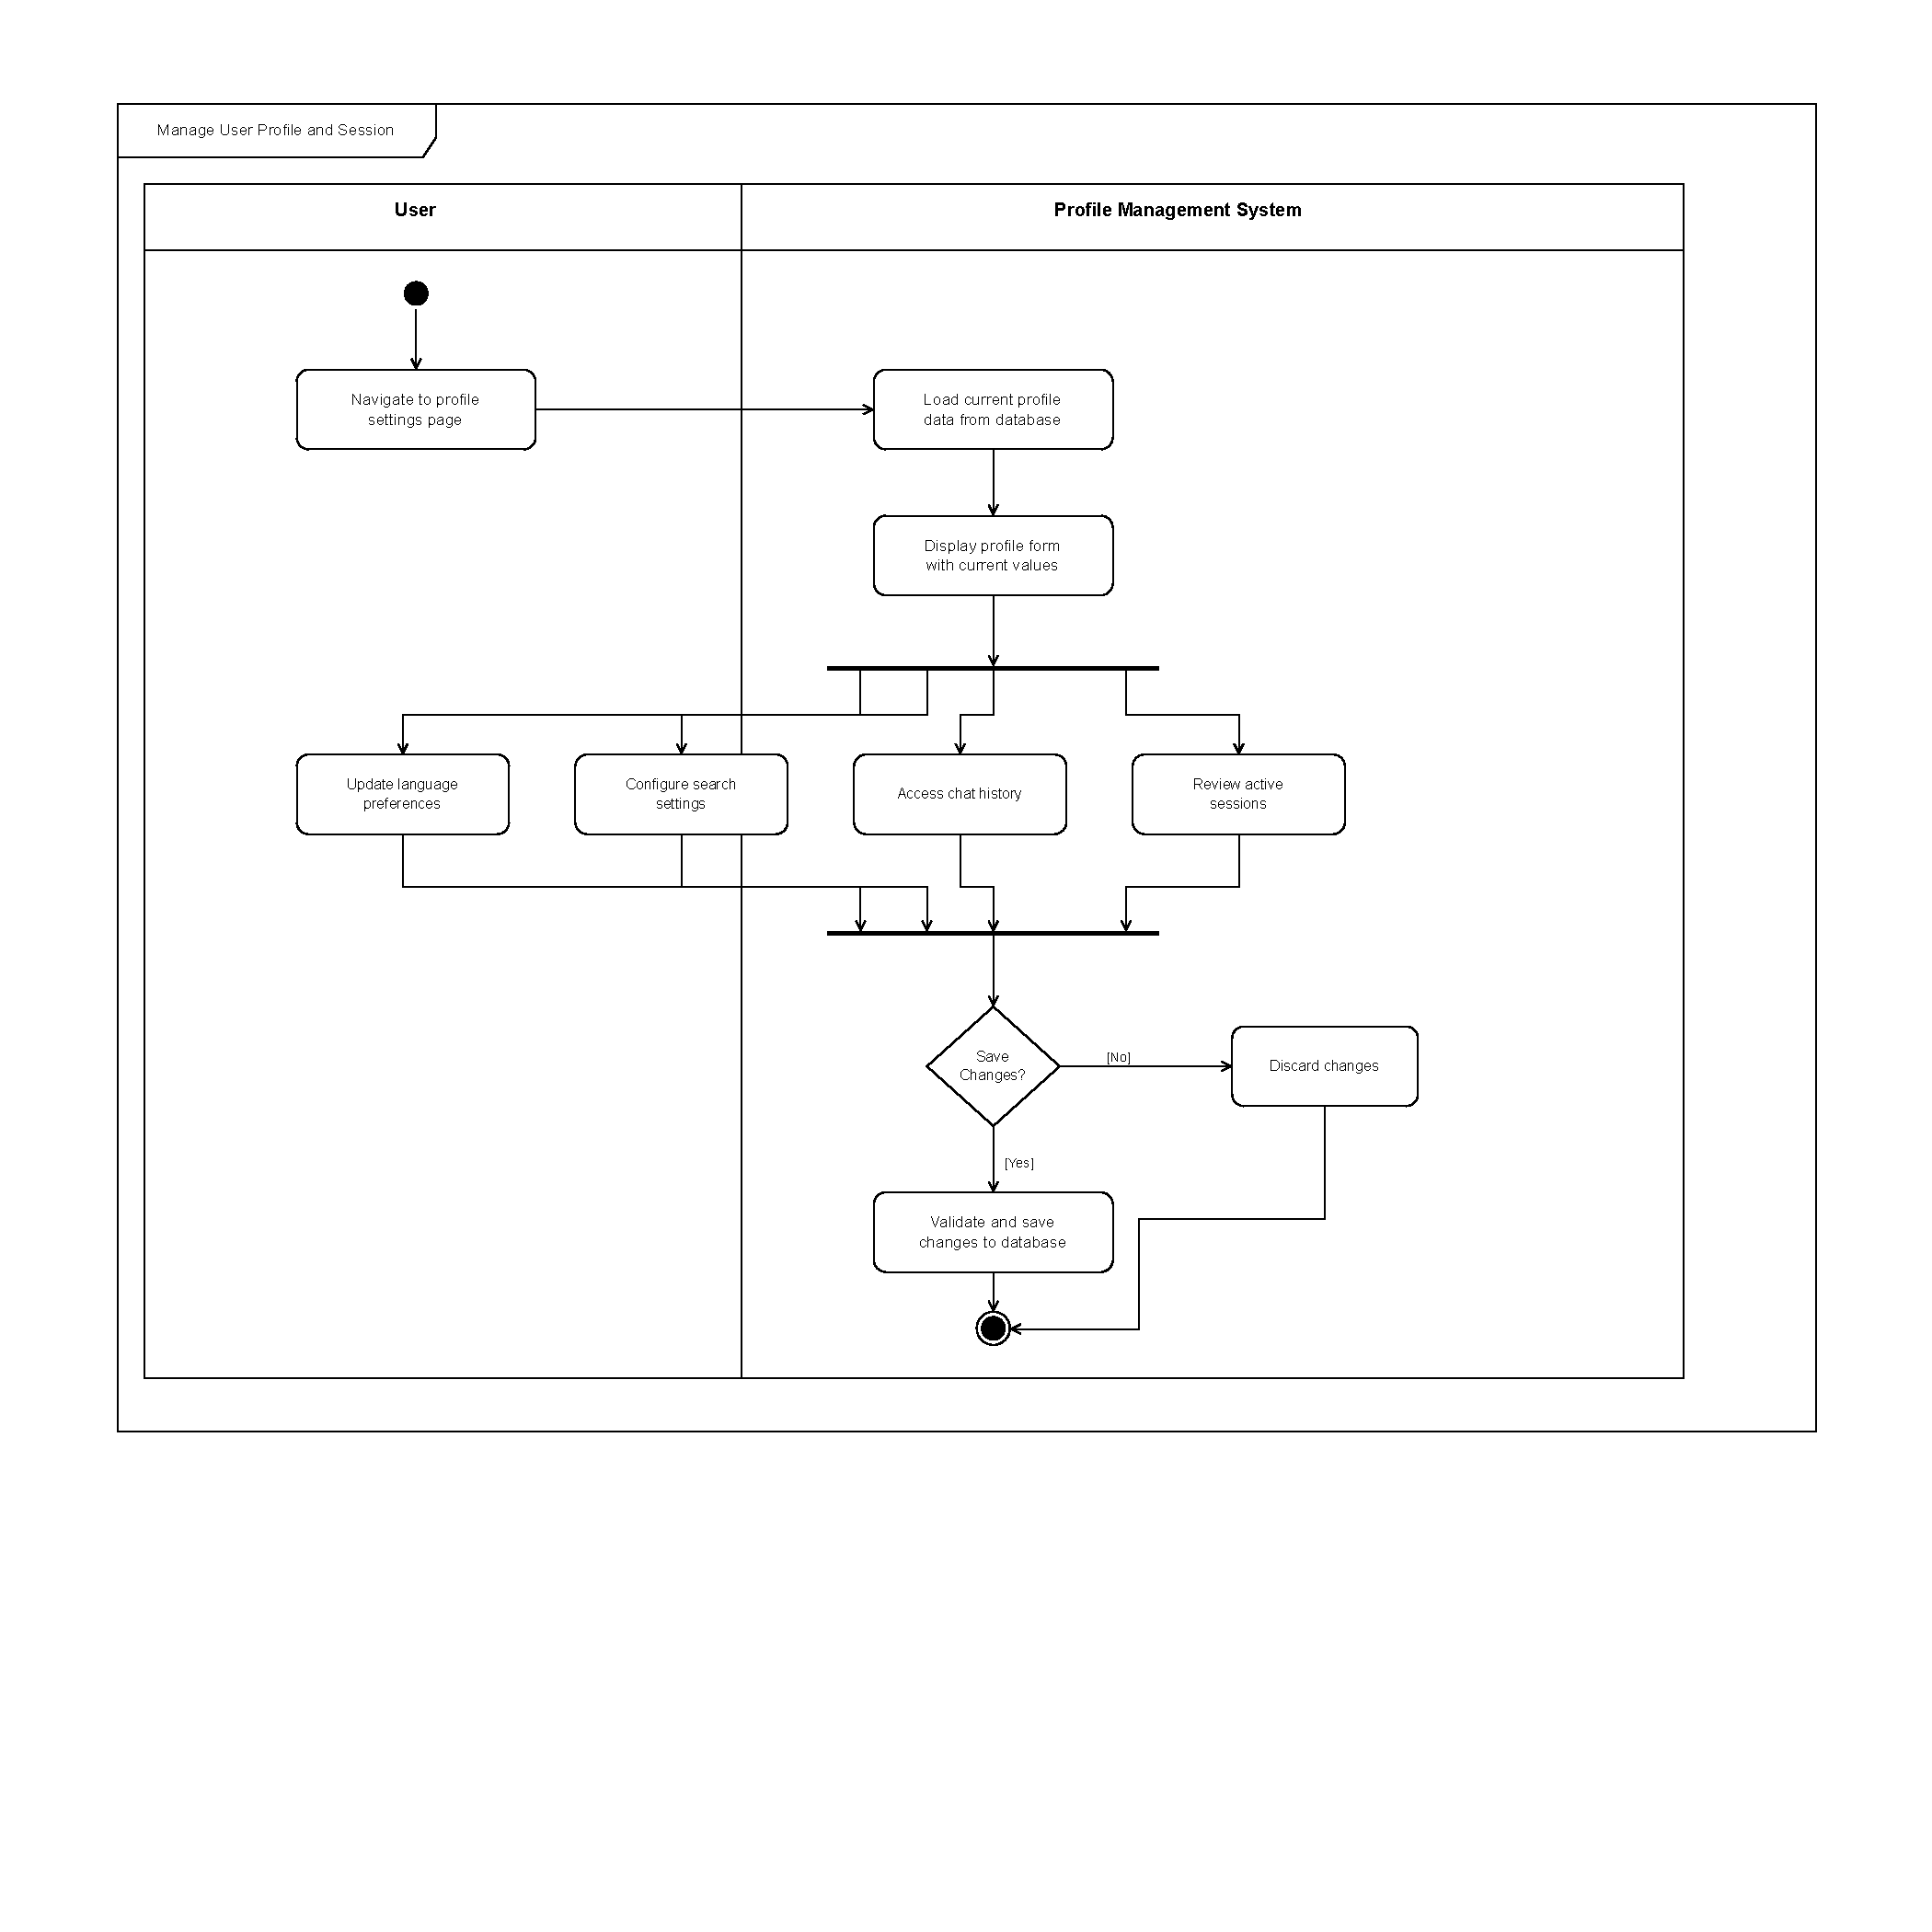
\includegraphics[width=0.55\linewidth]{activity2.drawio.pdf}
        \label{fig:placeholder}
    \end{figure}
\end{frame}

\begin{frame}{System Analysis and Design - Activity Diagram}
    \begin{figure}
        \centering
        \vspace{-3px}
        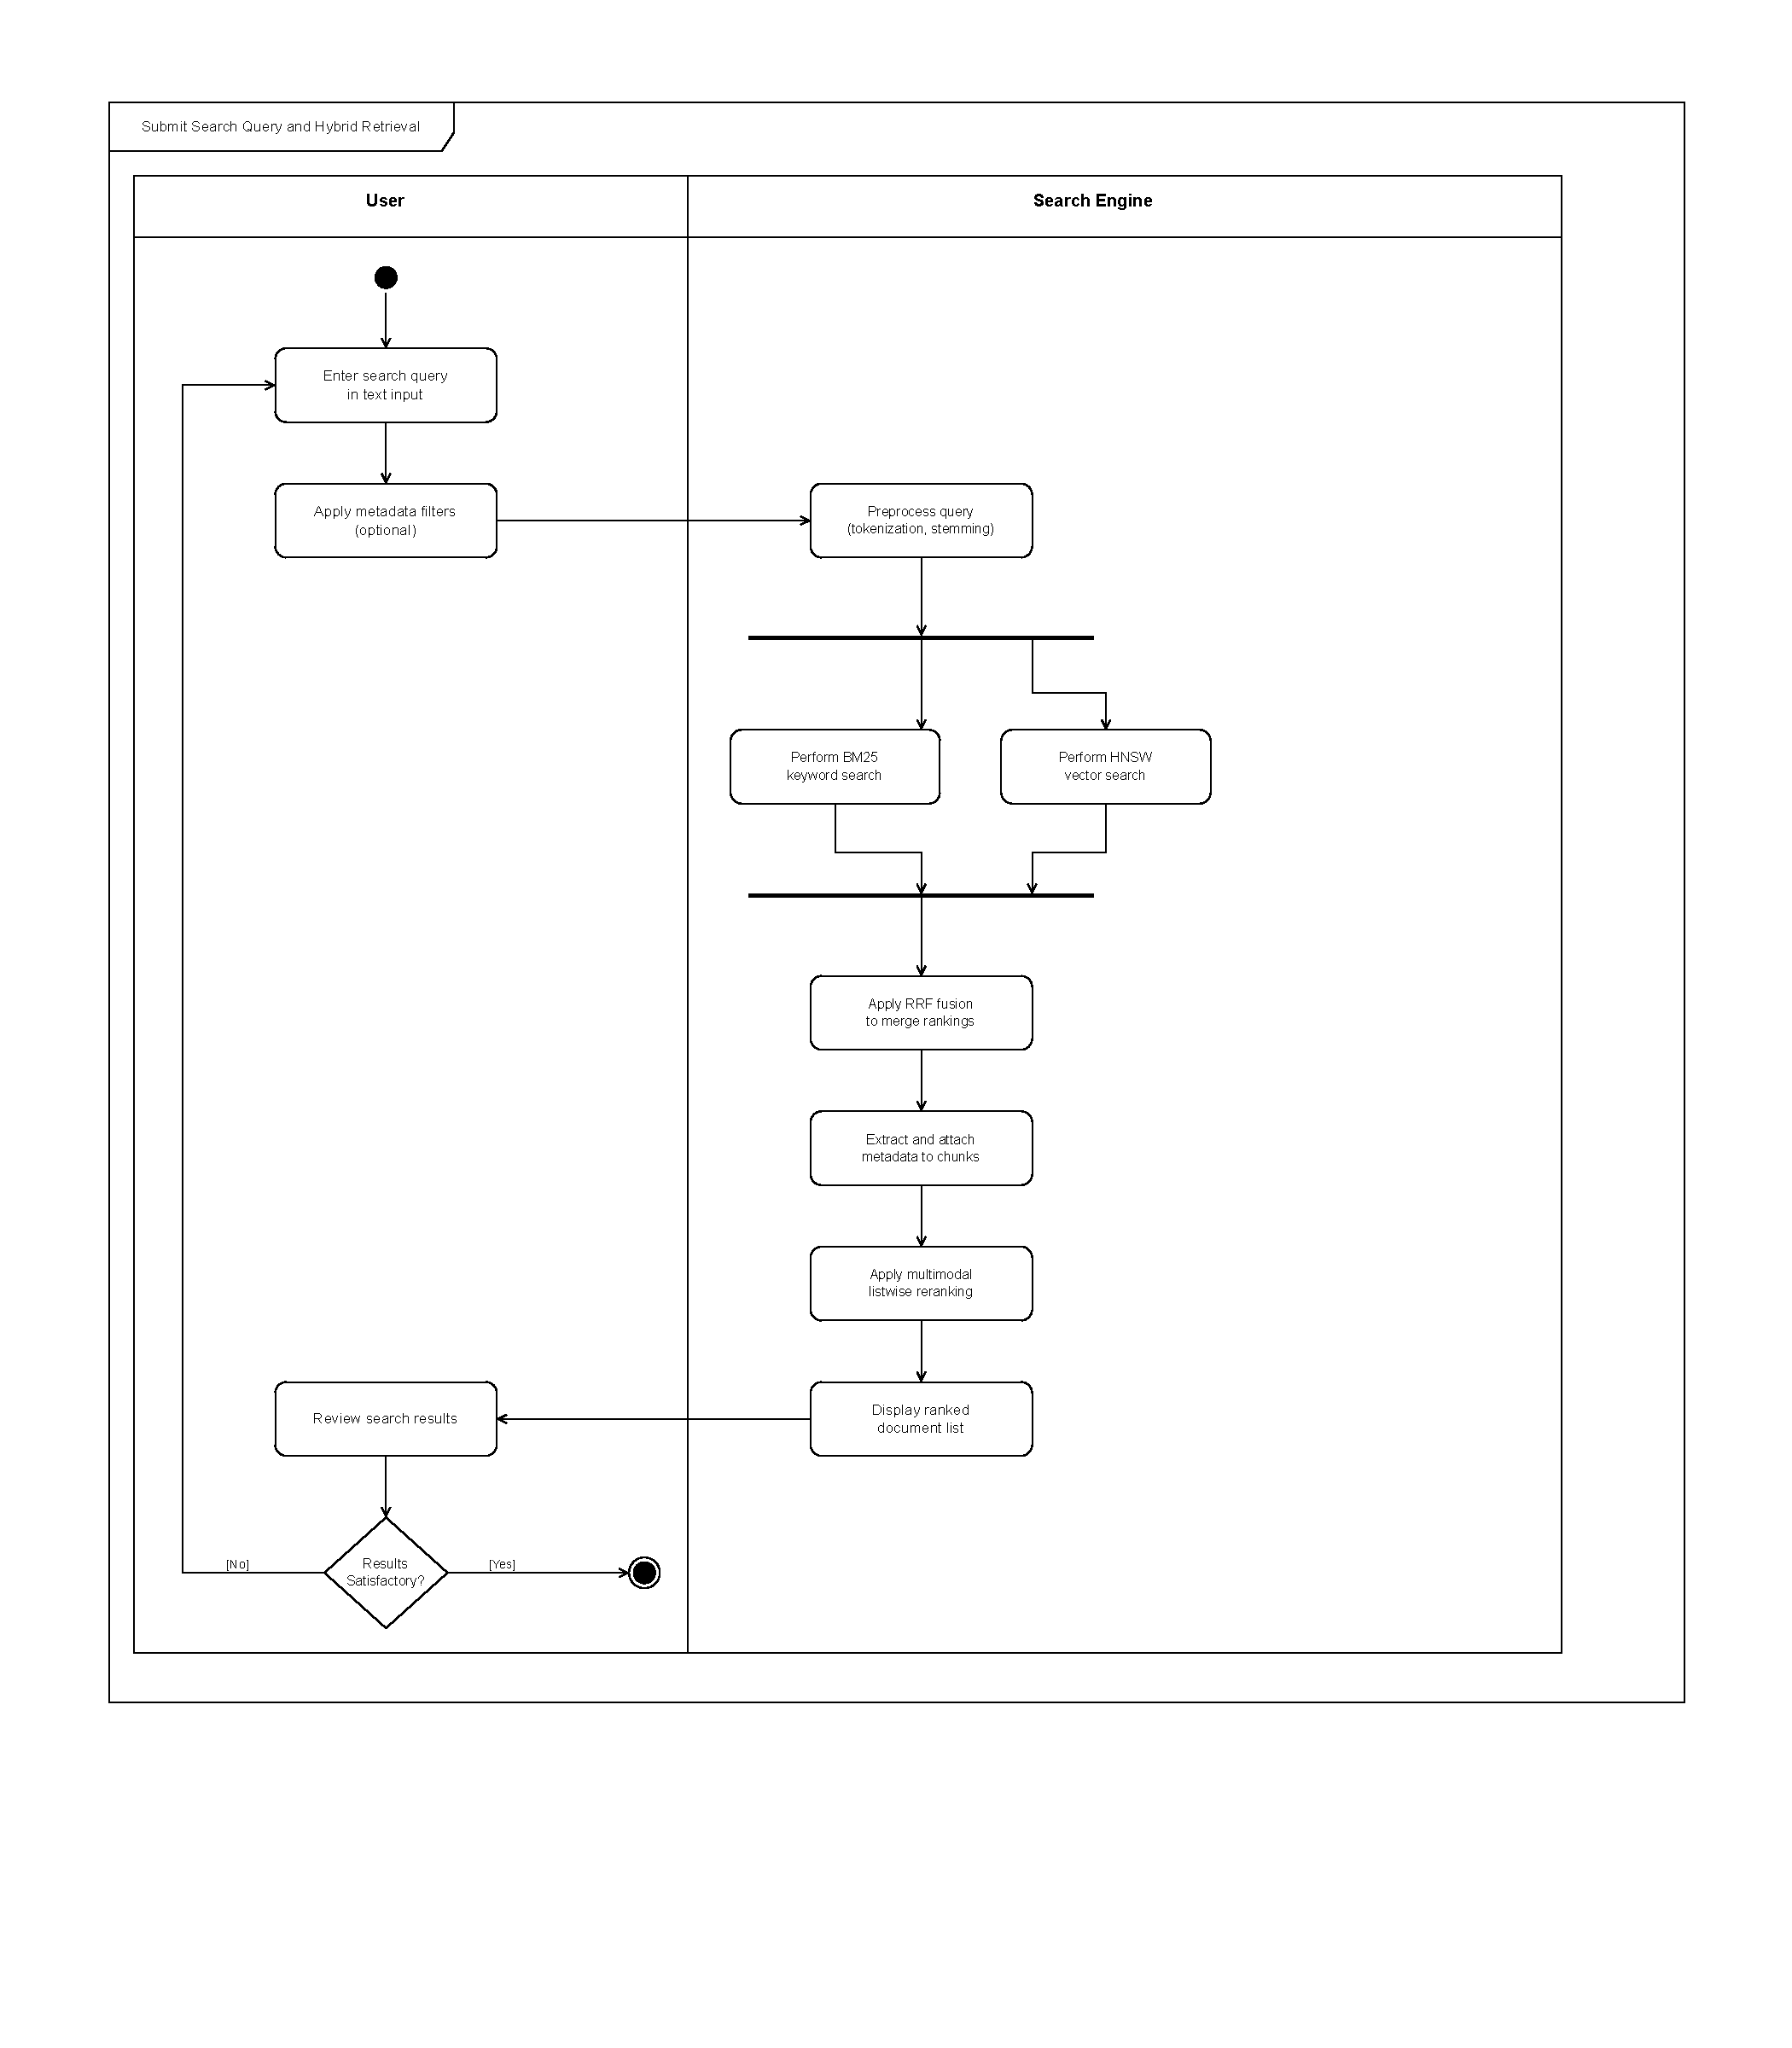
\includegraphics[width=0.55\linewidth]{activity3.drawio.pdf}
        \label{fig:placeholder}
    \end{figure}
\end{frame}

\begin{frame}{System Analysis and Design - Activity Diagram}
    \begin{figure}
        \centering
        \vspace{-3px}
        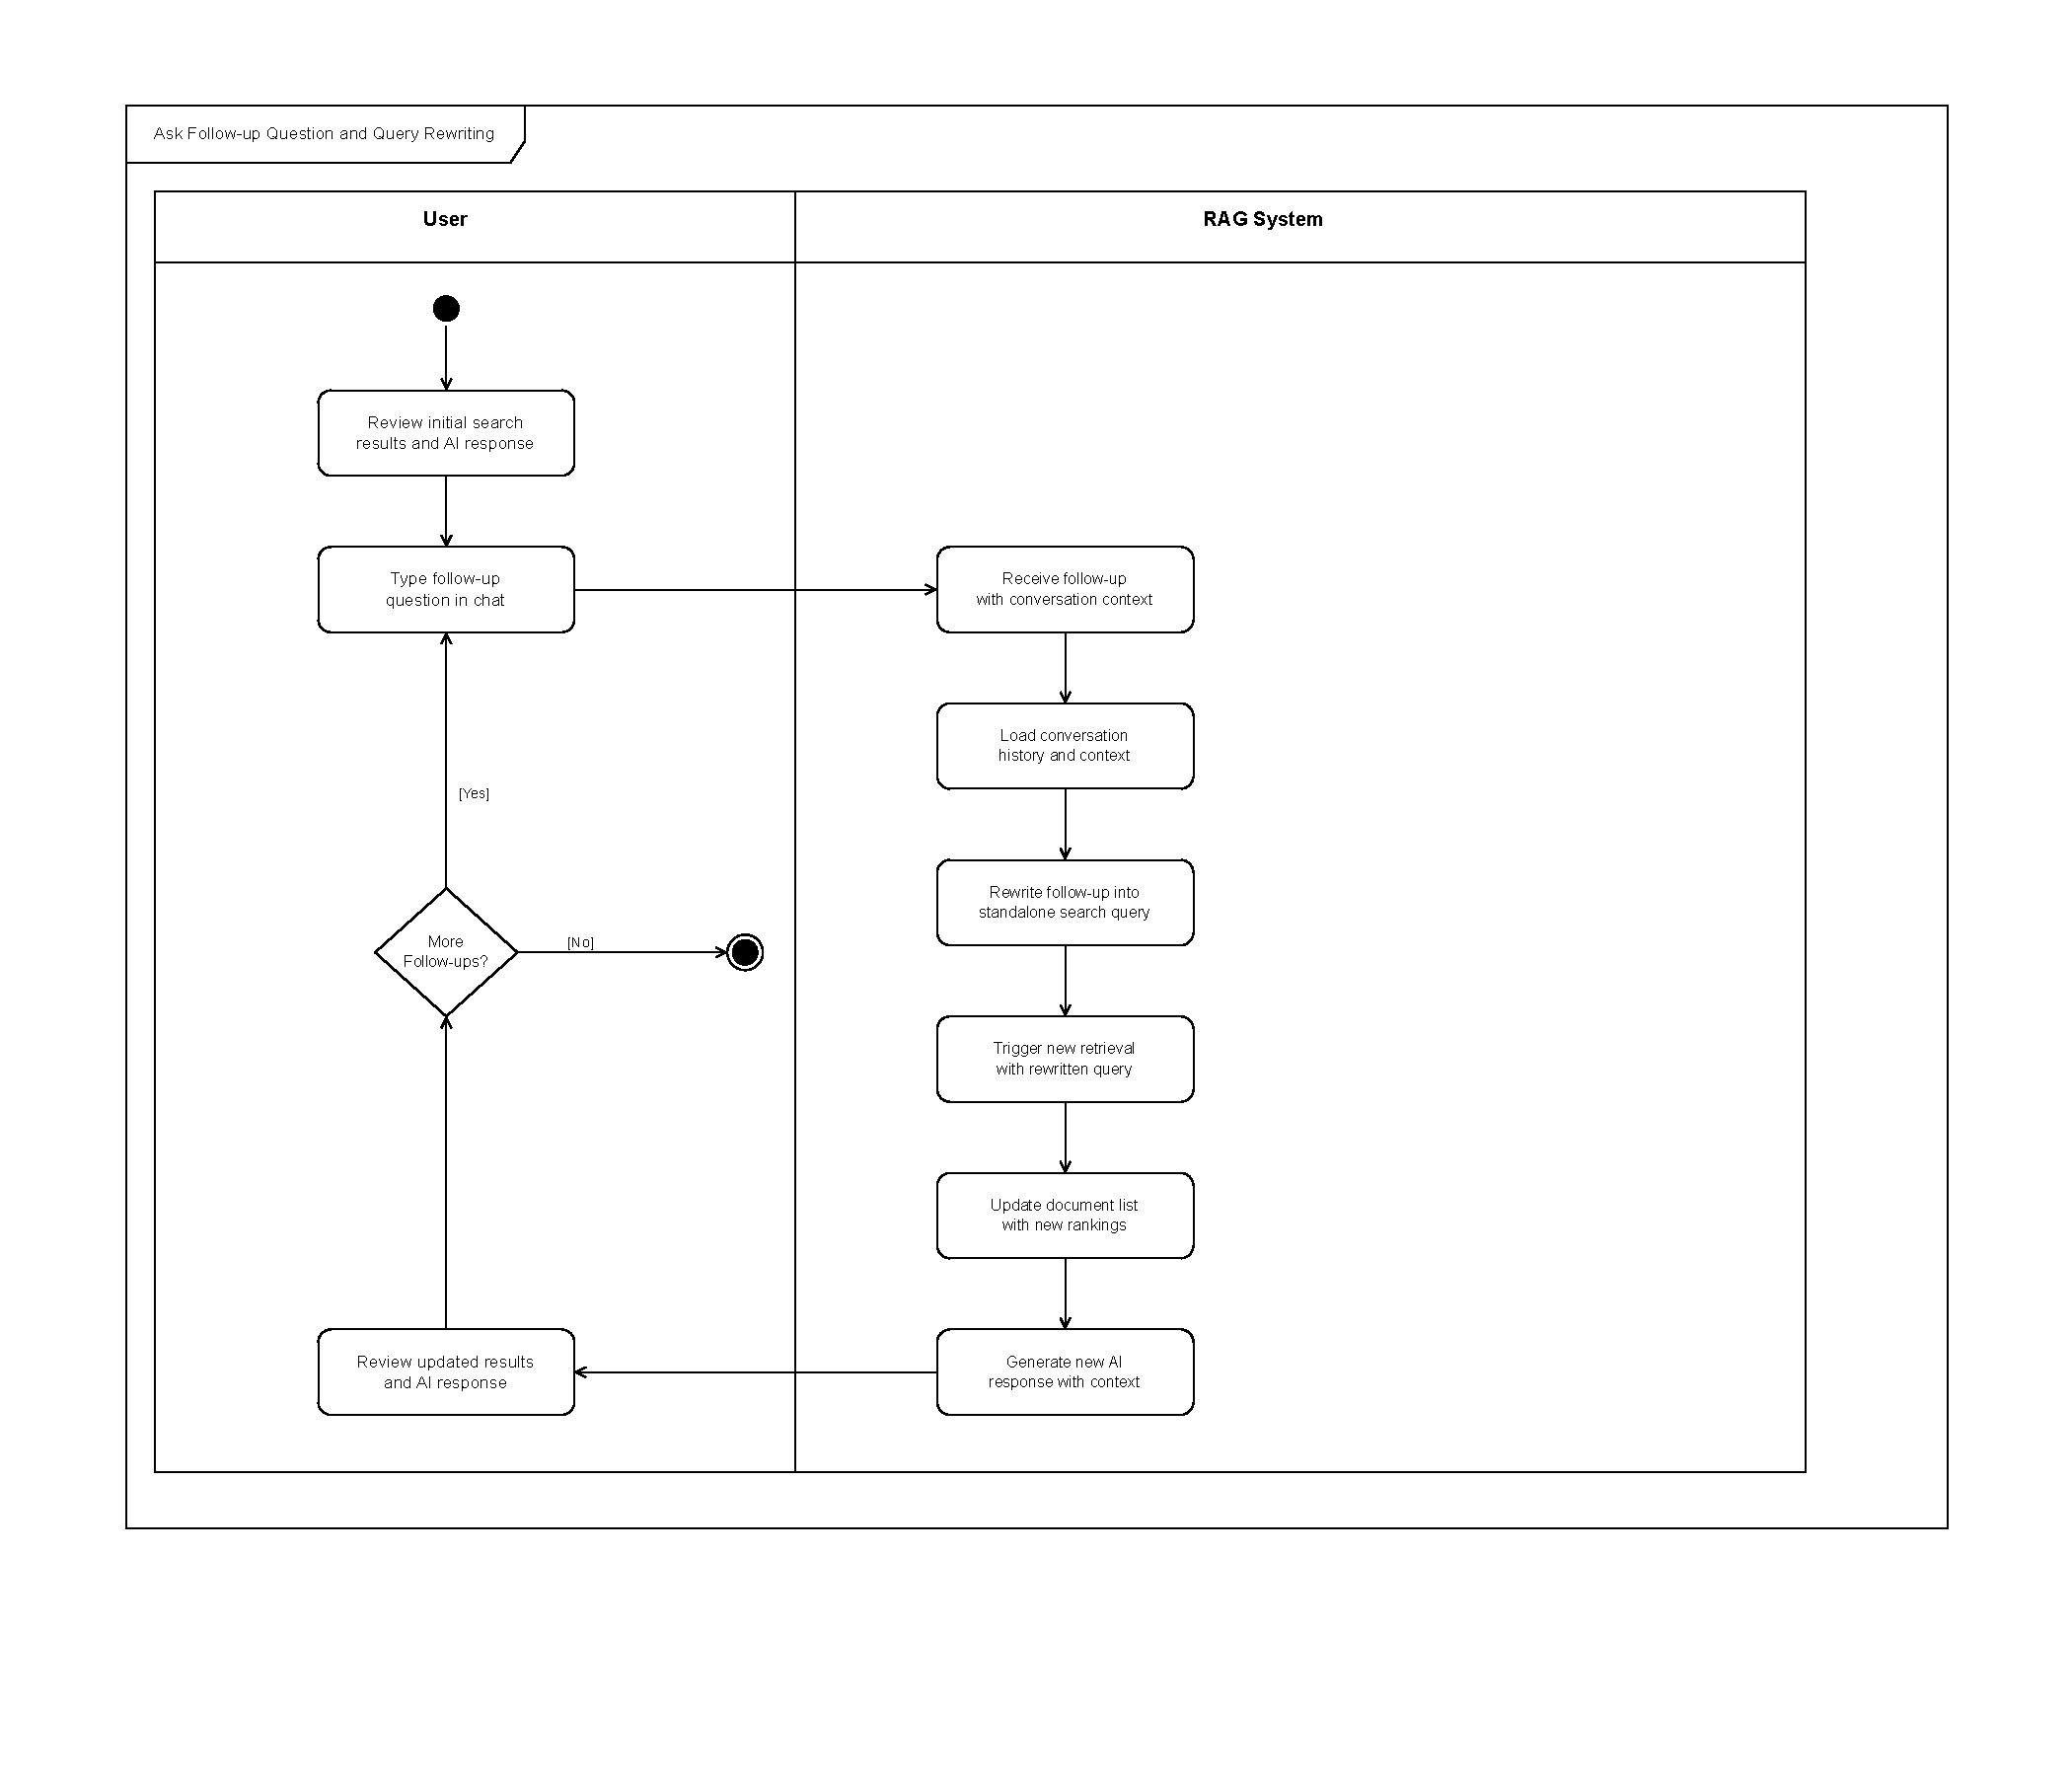
\includegraphics[width=0.55\linewidth]{activity4.drawio.pdf}
        \label{fig:placeholder}
    \end{figure}
\end{frame}

\begin{frame}{System Analysis and Design - Activity Diagram}
    \begin{figure}
        \centering
        \vspace{-3px}
        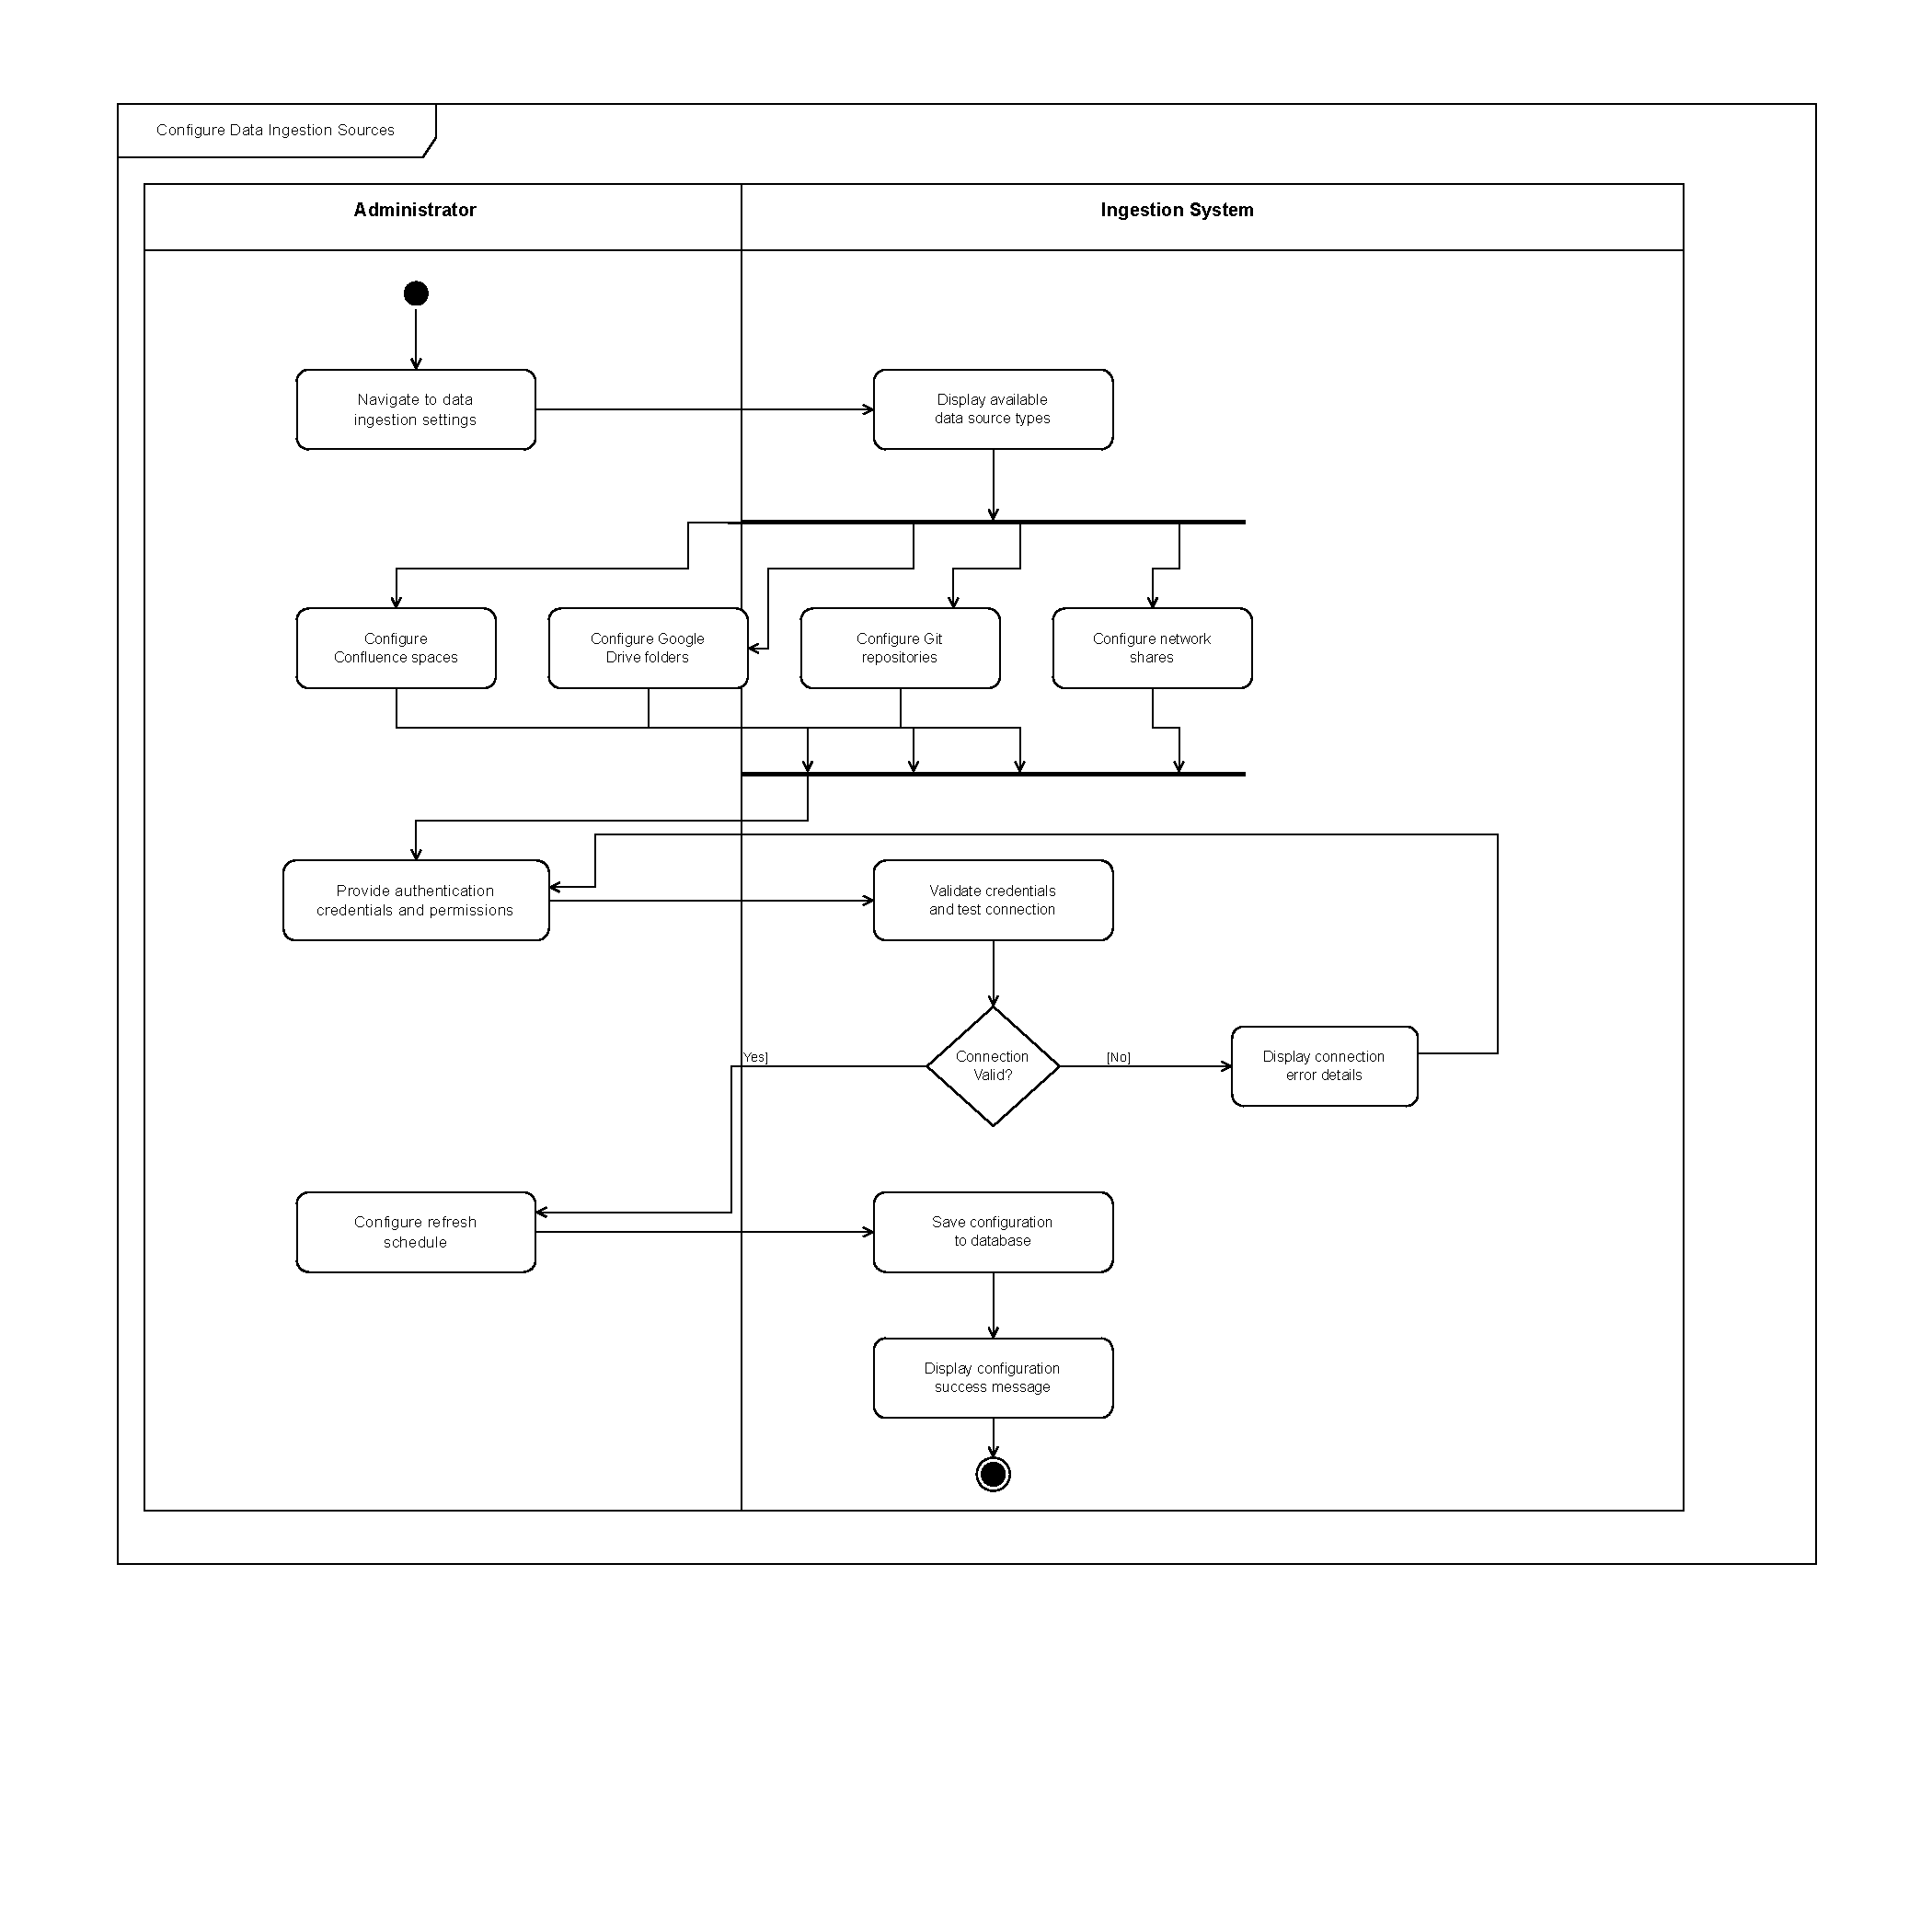
\includegraphics[width=0.55\linewidth]{activity5.drawio.pdf}
        \label{fig:placeholder}
    \end{figure}
\end{frame}

\begin{frame}{System Analysis and Design - Activity Diagram}
    \begin{figure}
        \centering
        \vspace{-3px}
        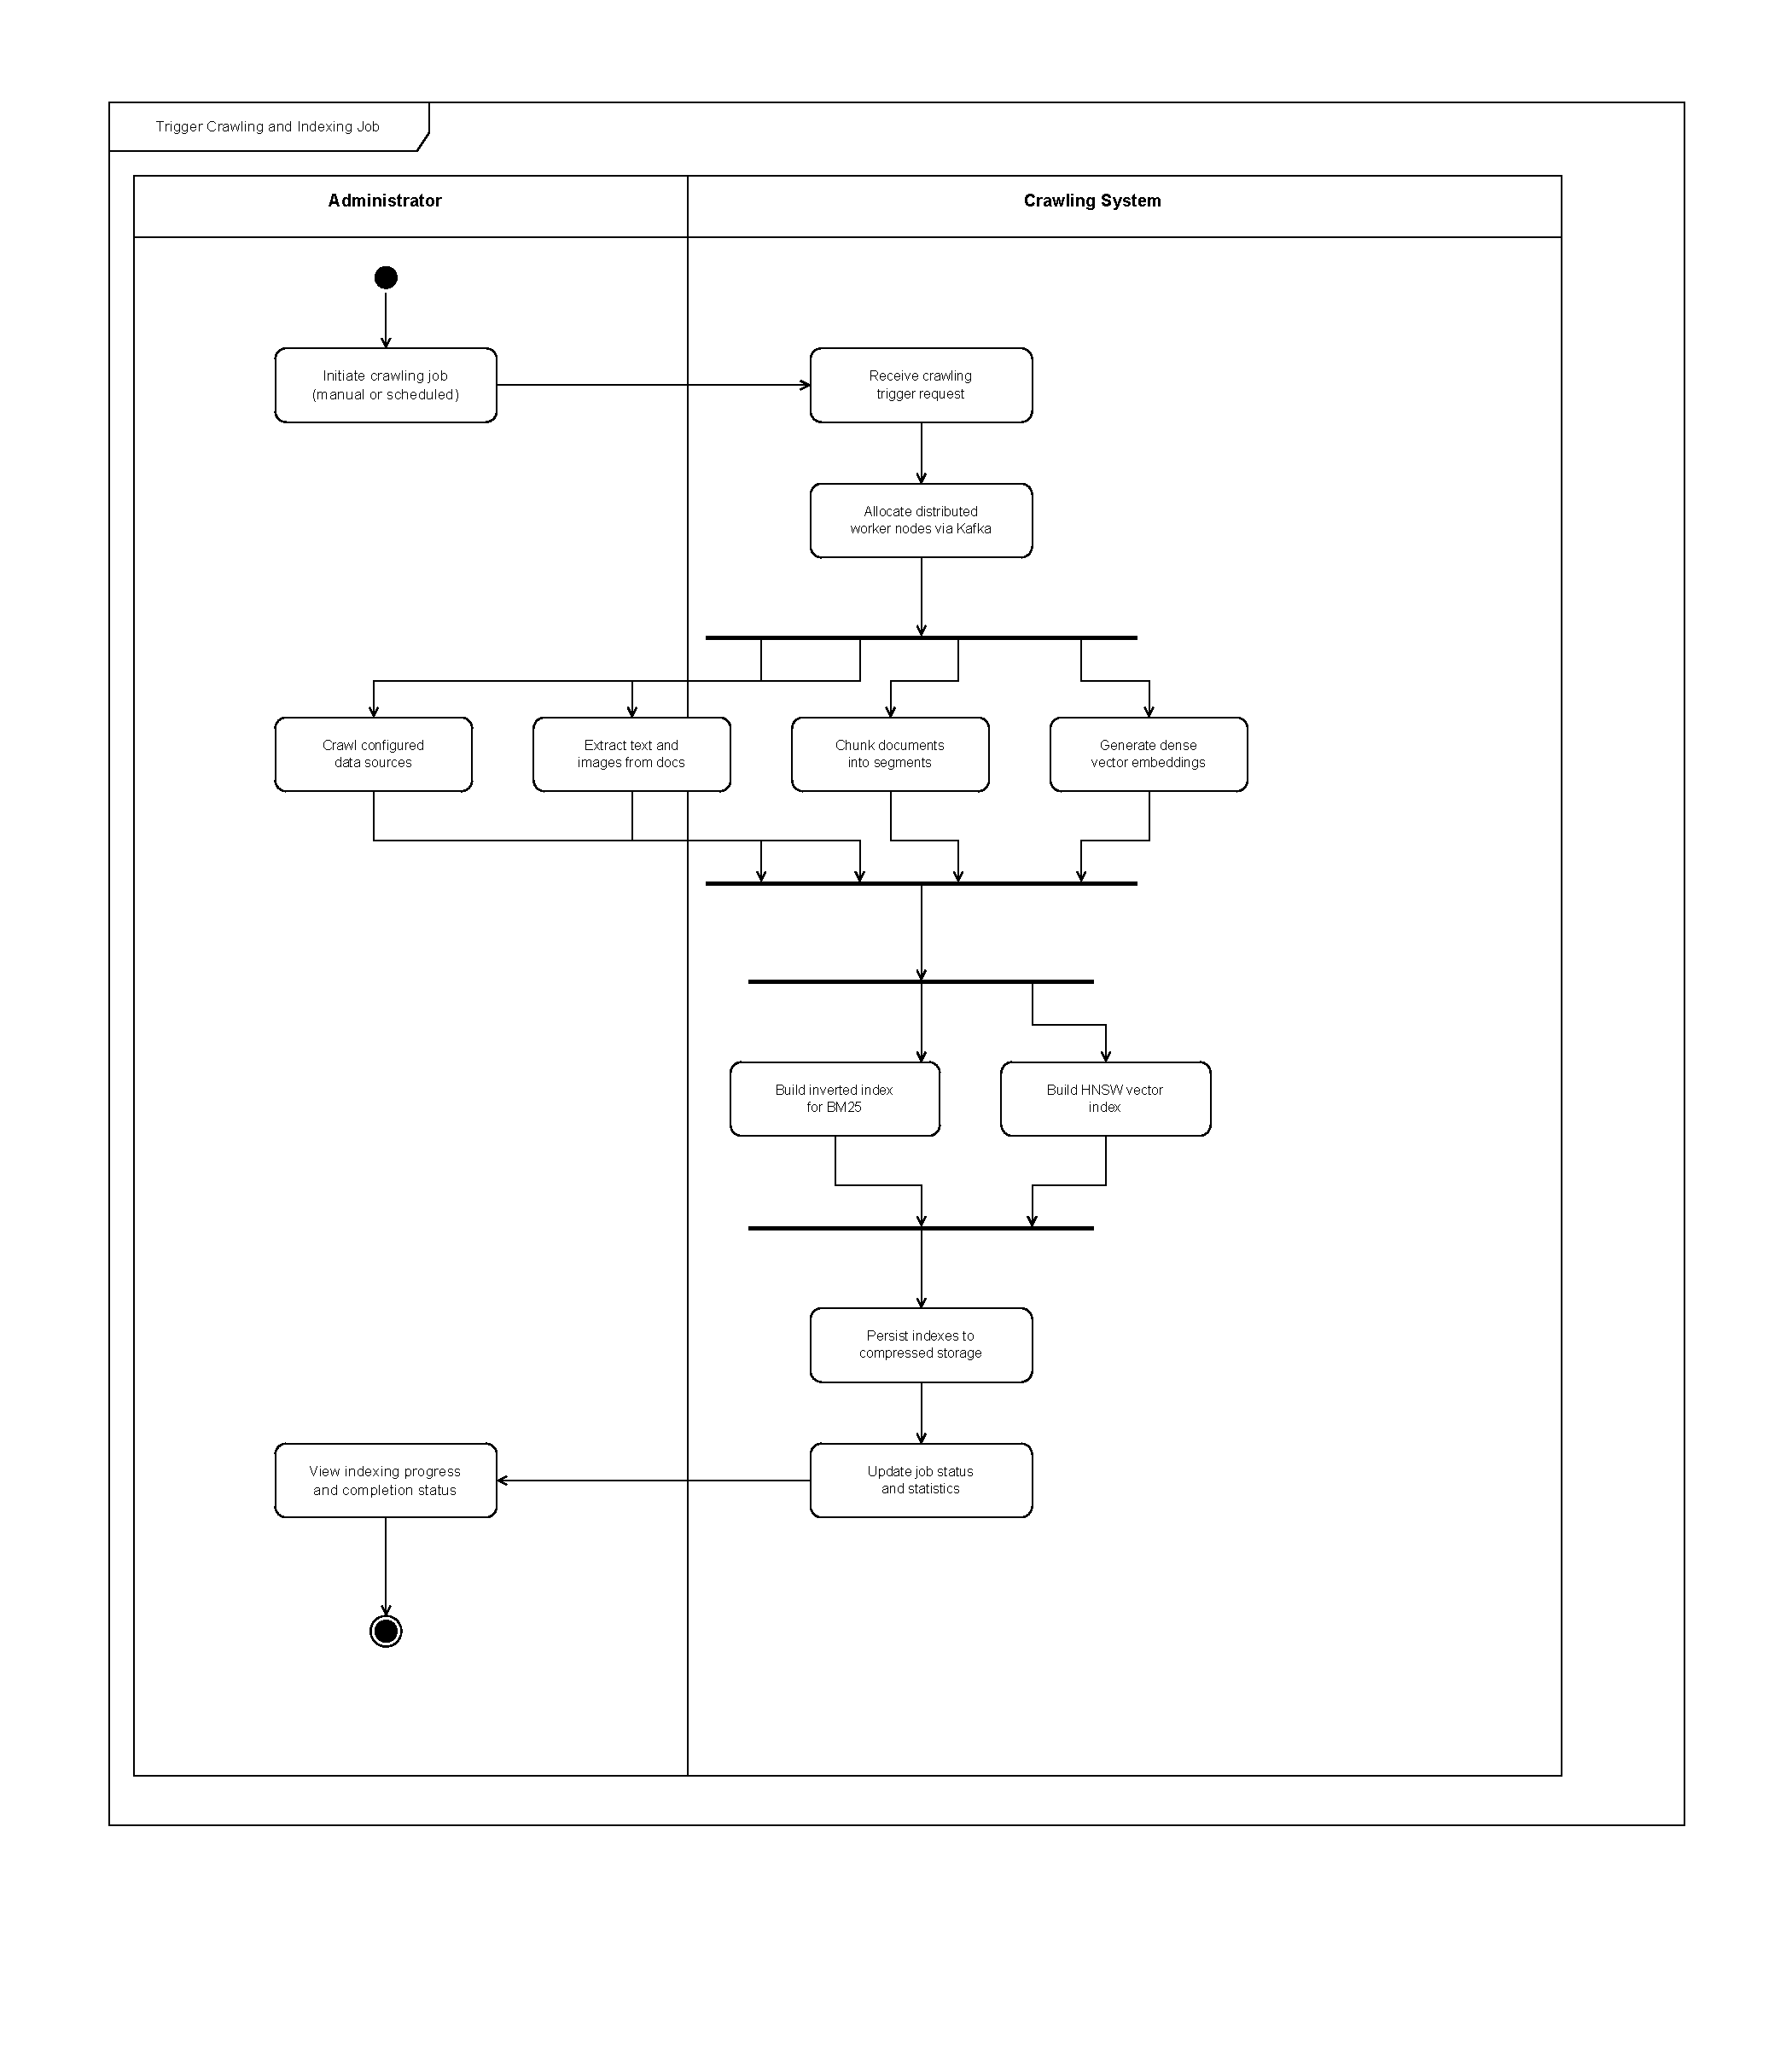
\includegraphics[width=0.55\linewidth]{activity6.drawio.pdf}
        \label{fig:placeholder}
    \end{figure}
\end{frame}

\begin{frame}{System Analysis and Design - Activity Diagram}
    \begin{figure}
        \centering
        \vspace{-3px}
        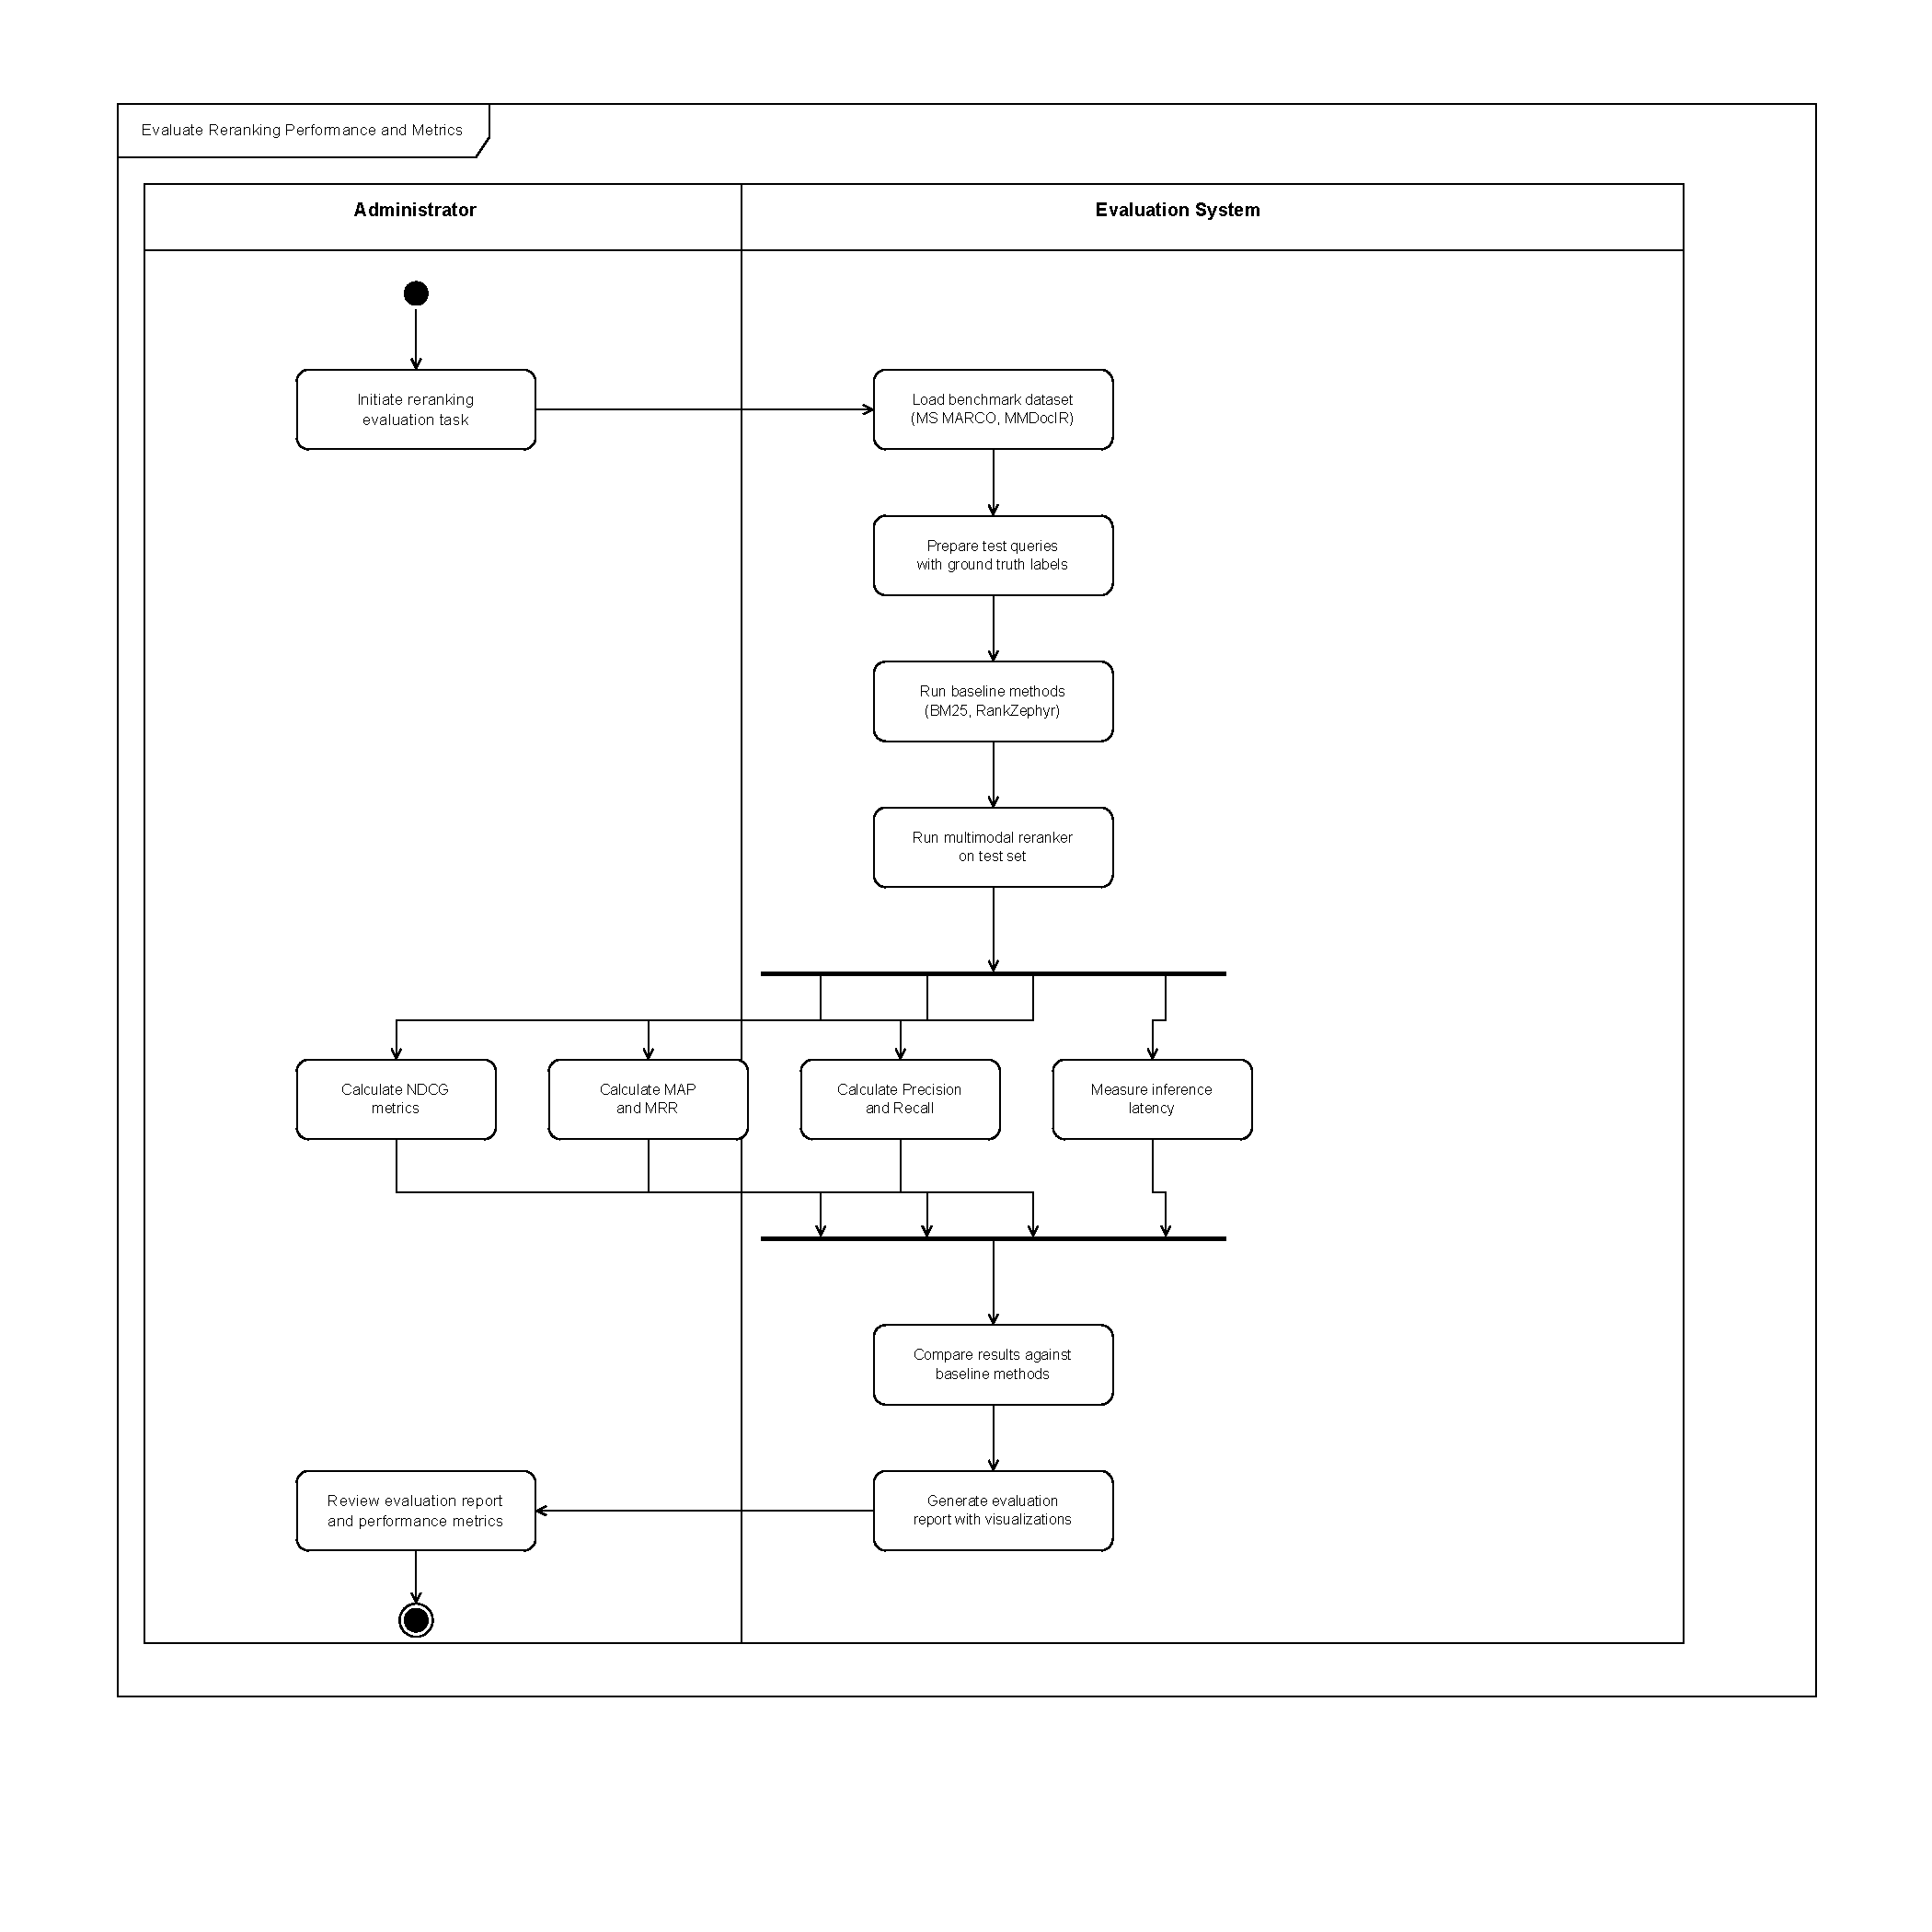
\includegraphics[width=0.55\linewidth]{activity7.drawio.pdf}
        \label{fig:placeholder}
    \end{figure}
\end{frame}

\begin{frame}{System Analysis and Design - Activity Diagram}
    \begin{figure}
        \centering
        \vspace{-3px}
        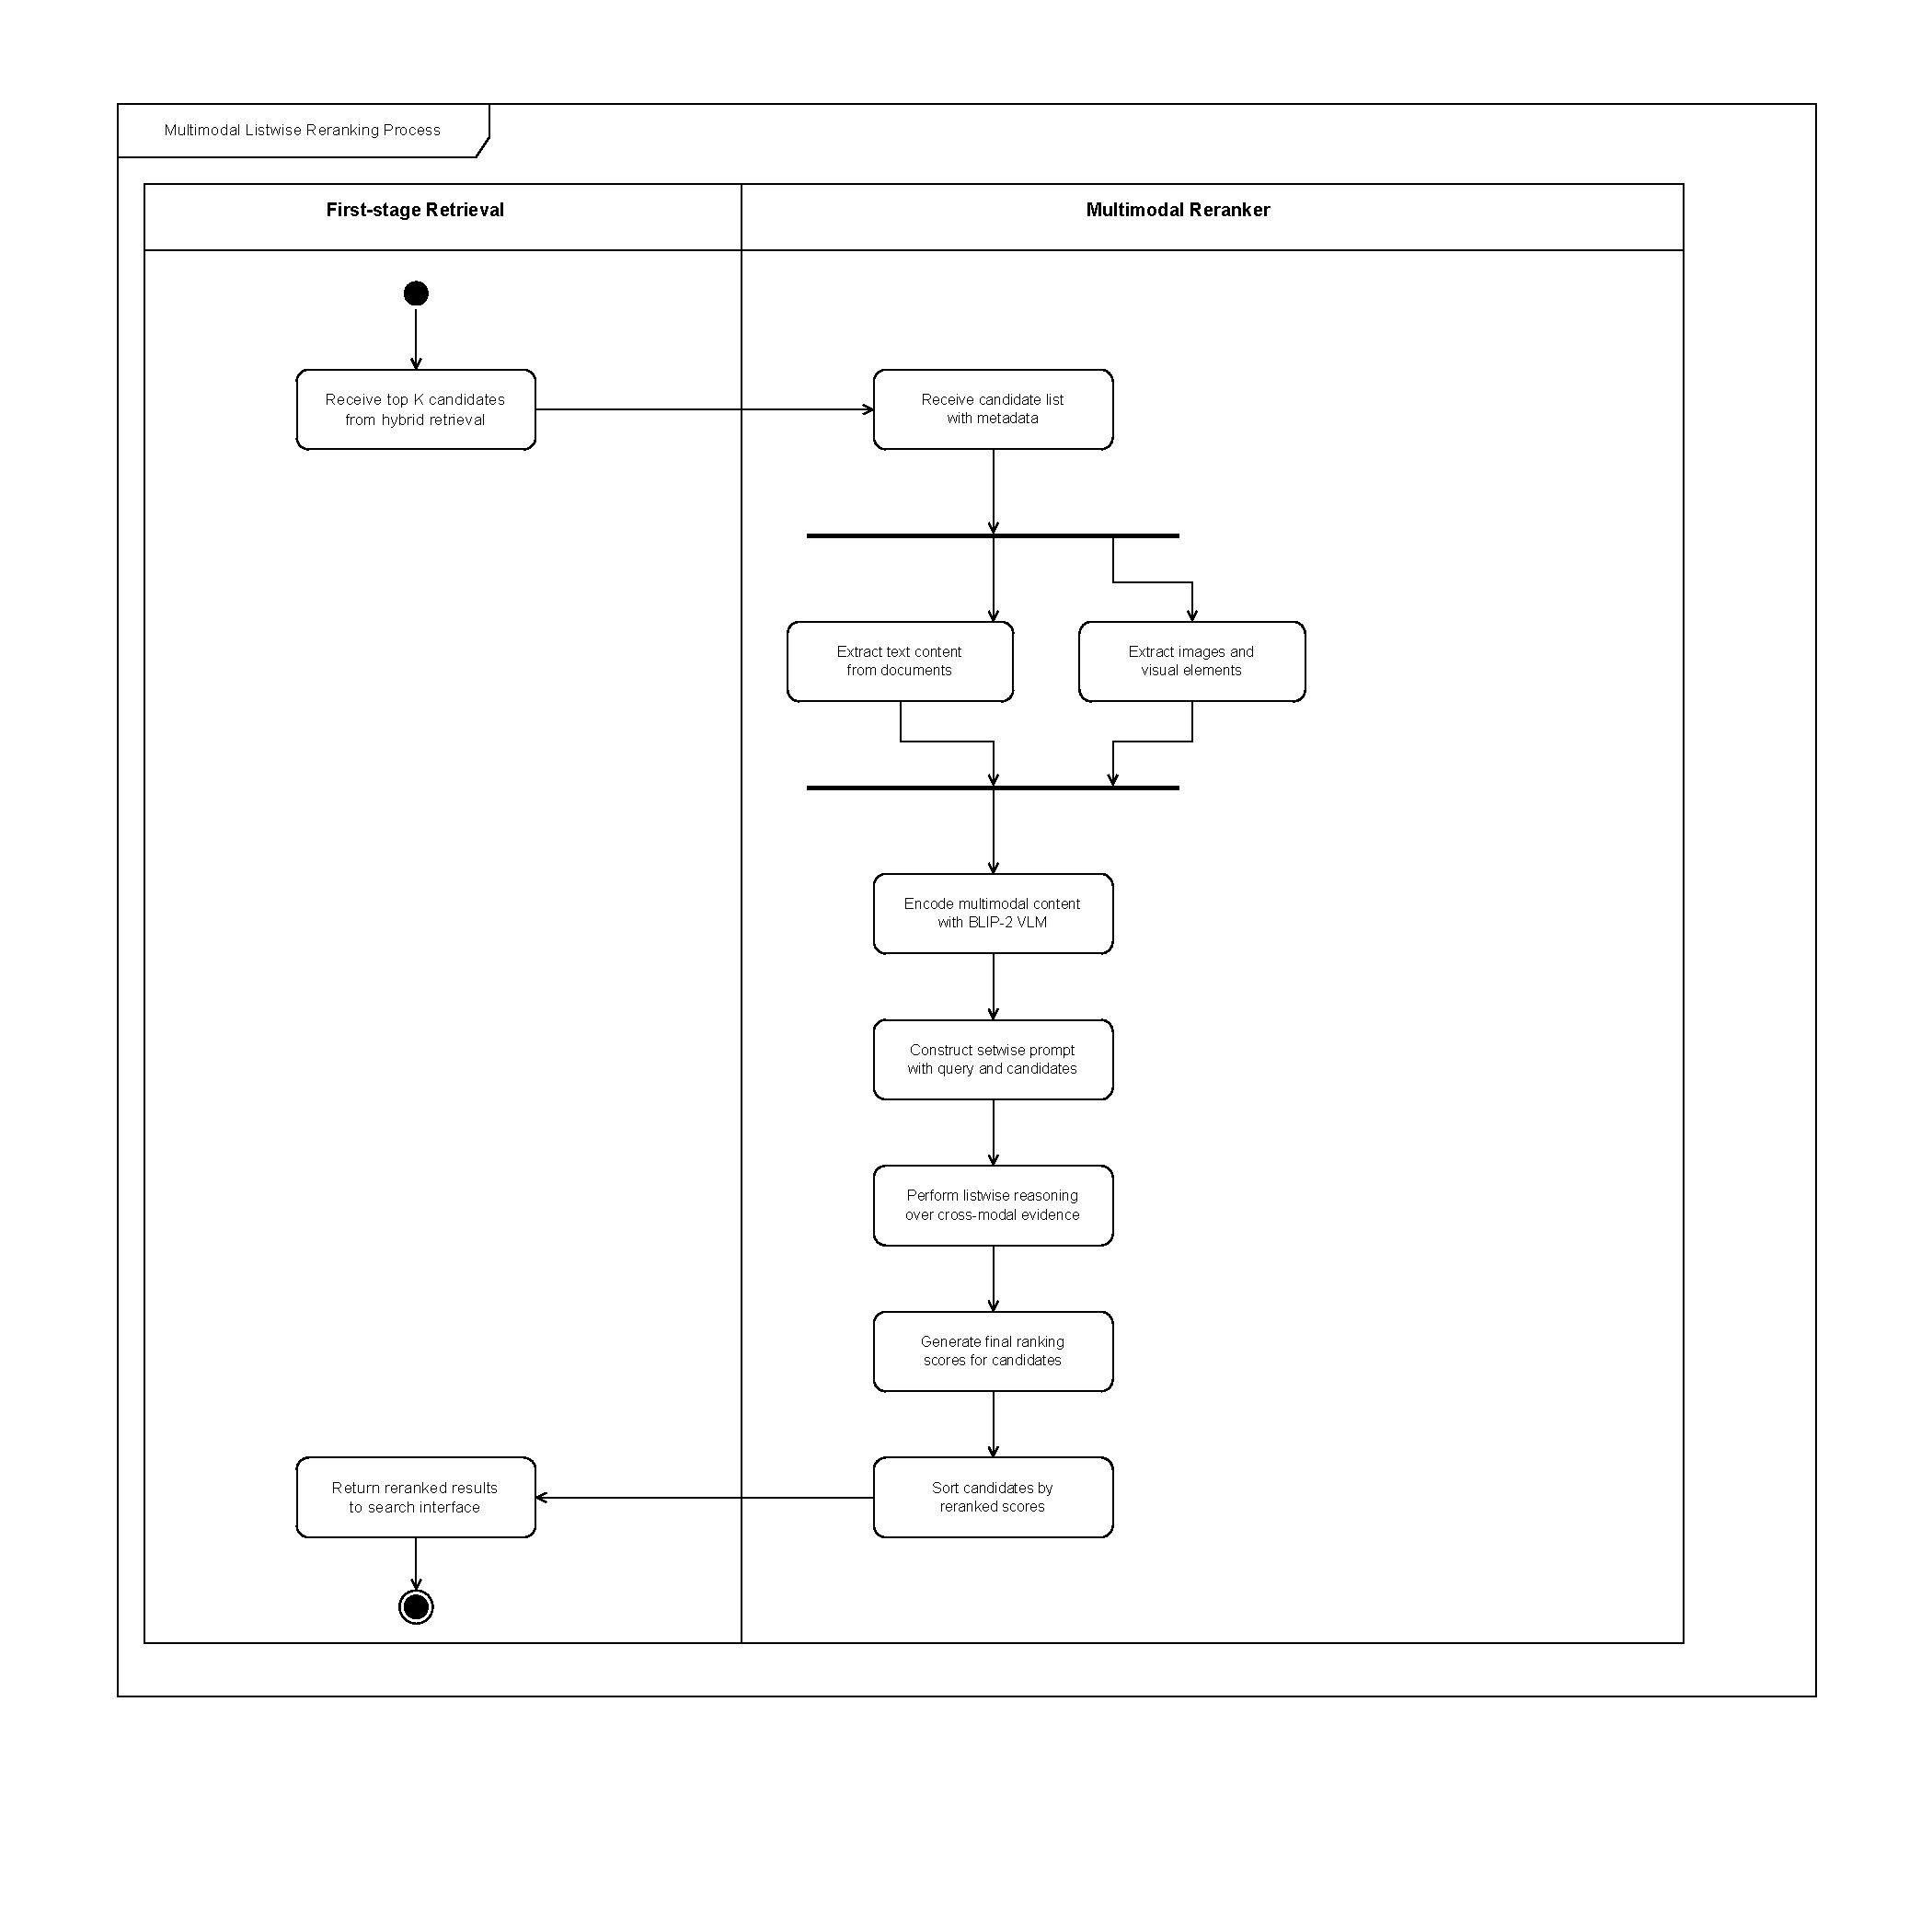
\includegraphics[width=0.55\linewidth]{activity8.drawio.pdf}
        \label{fig:placeholder}
    \end{figure}
\end{frame}

\begin{frame}{System Analysis and Design - Activity Diagram}
    \begin{figure}
        \centering
        \vspace{-3px}
        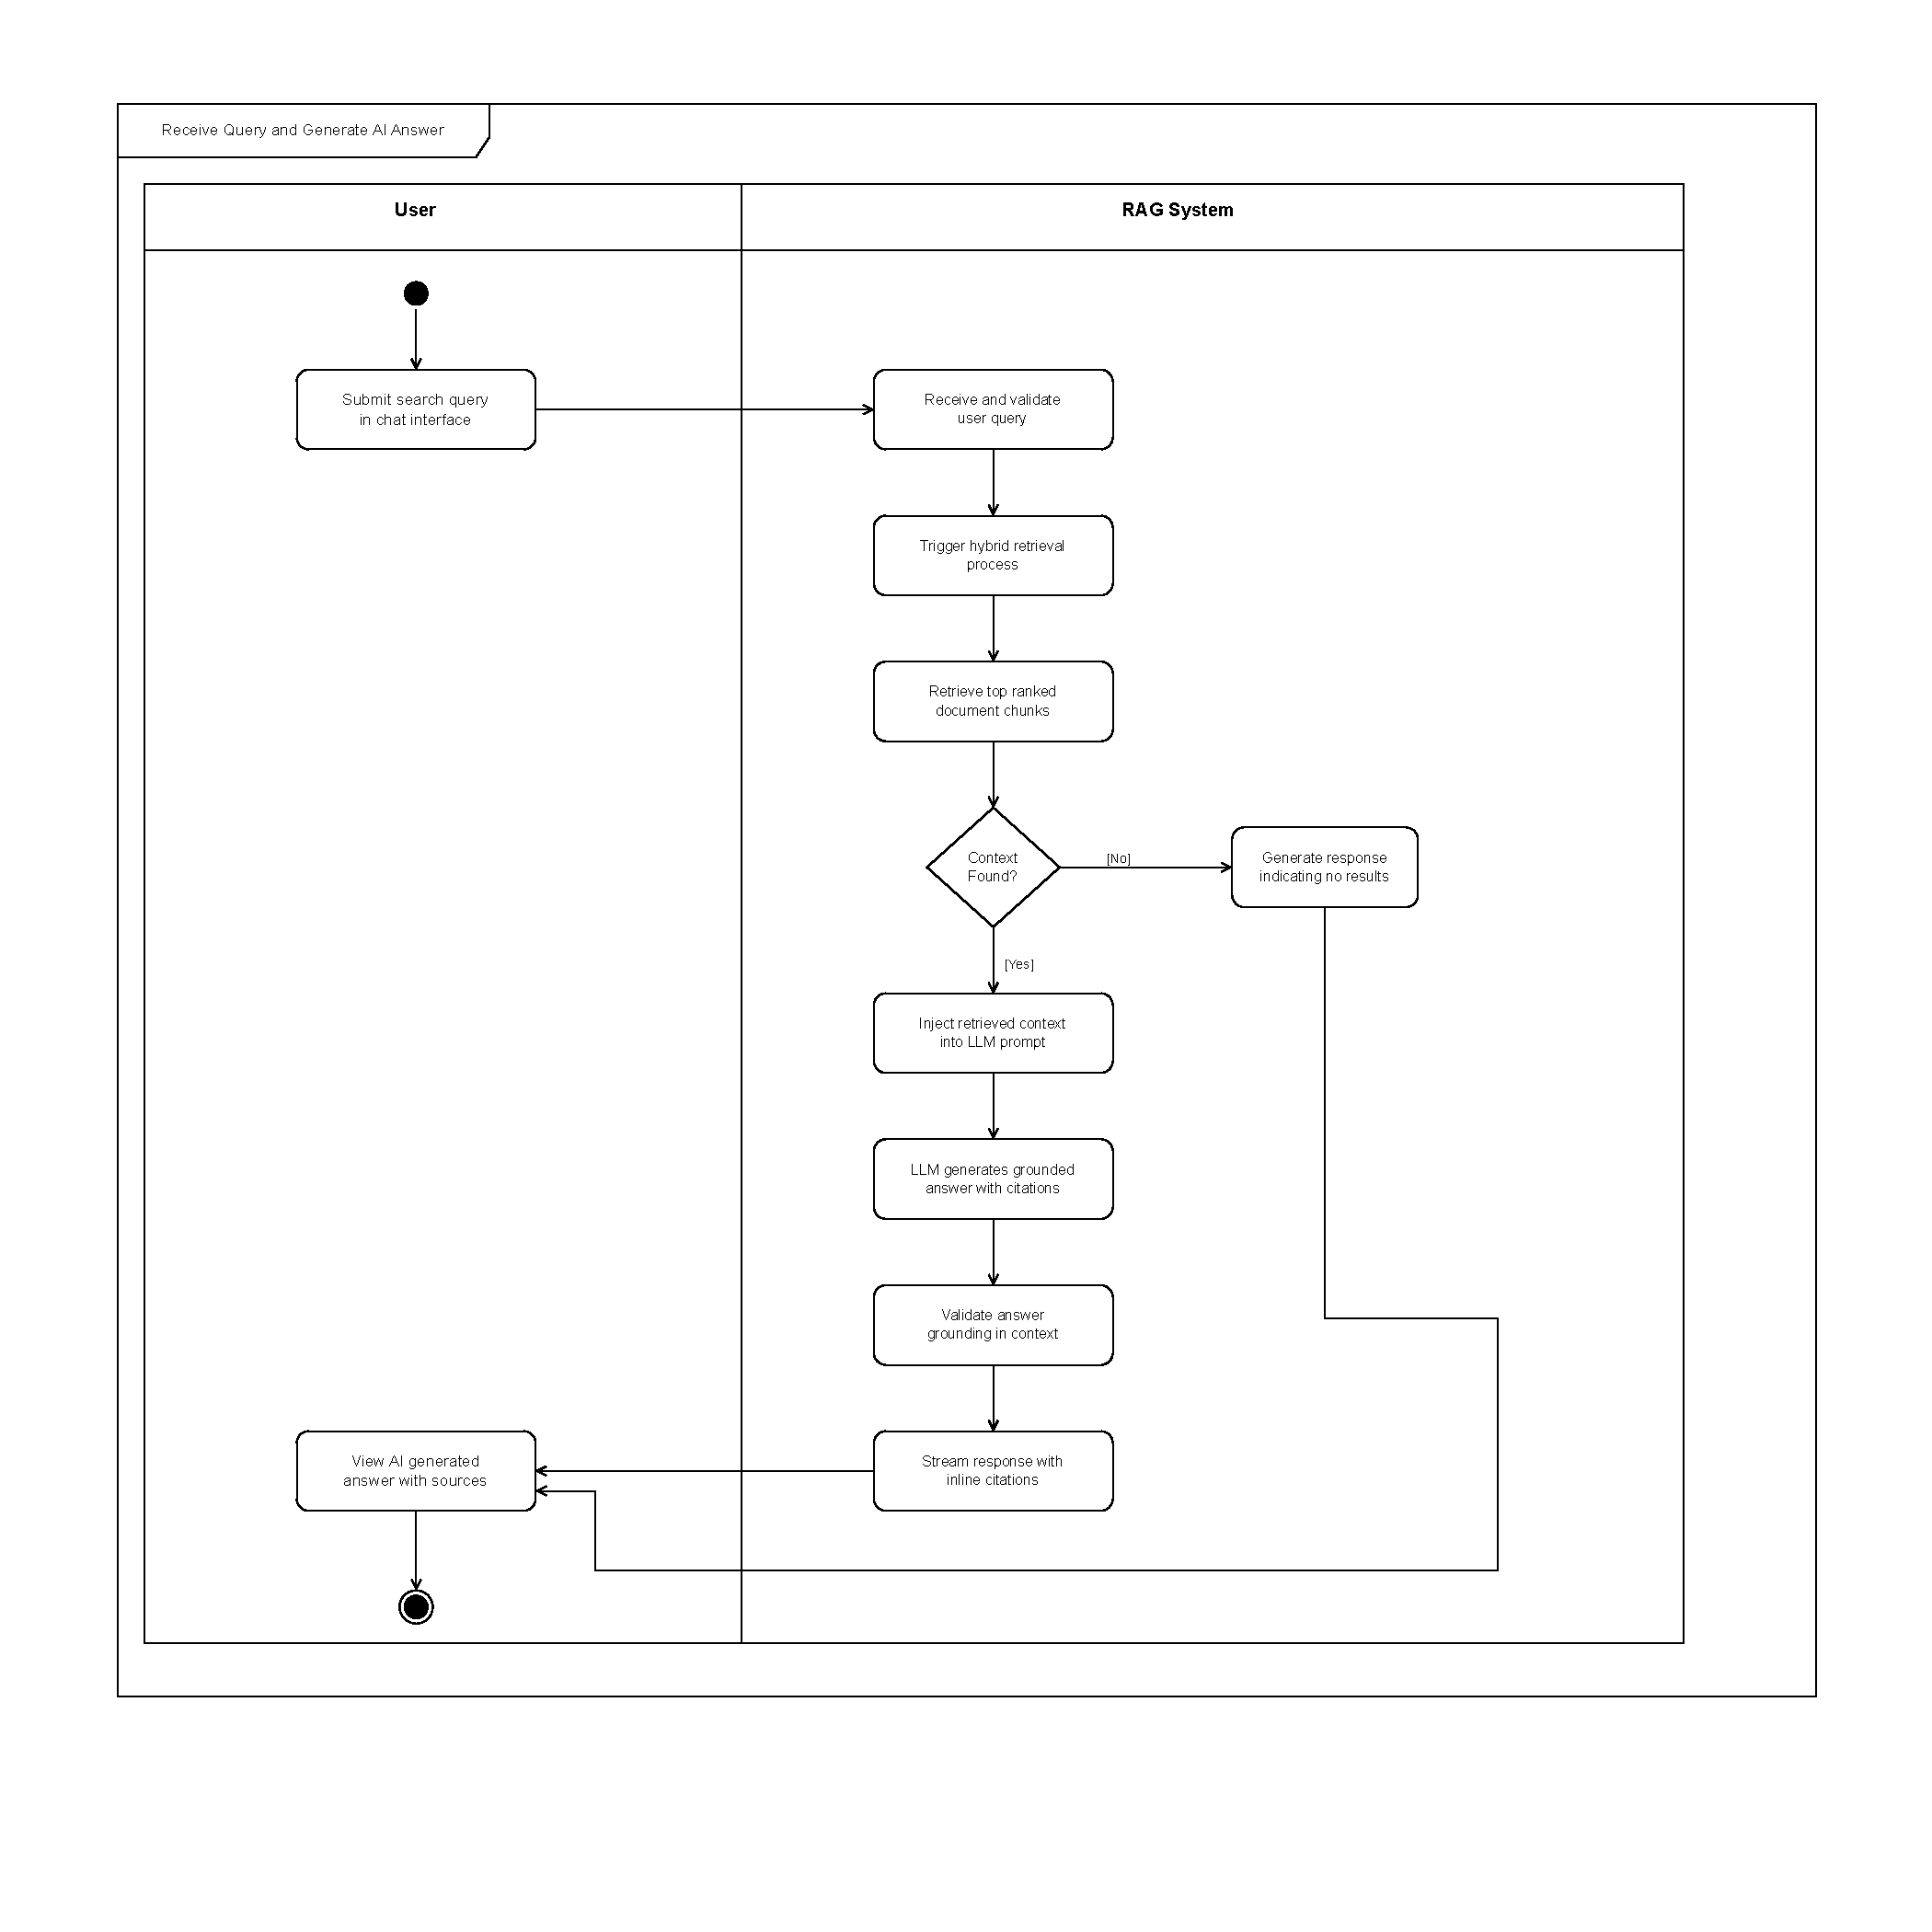
\includegraphics[width=0.55\linewidth]{activity9.drawio.pdf}
        \label{fig:placeholder}
    \end{figure}
\end{frame}

\begin{frame}{System Analysis and Design - Activity Diagram}
    \begin{figure}
        \centering
        \vspace{-3px}
        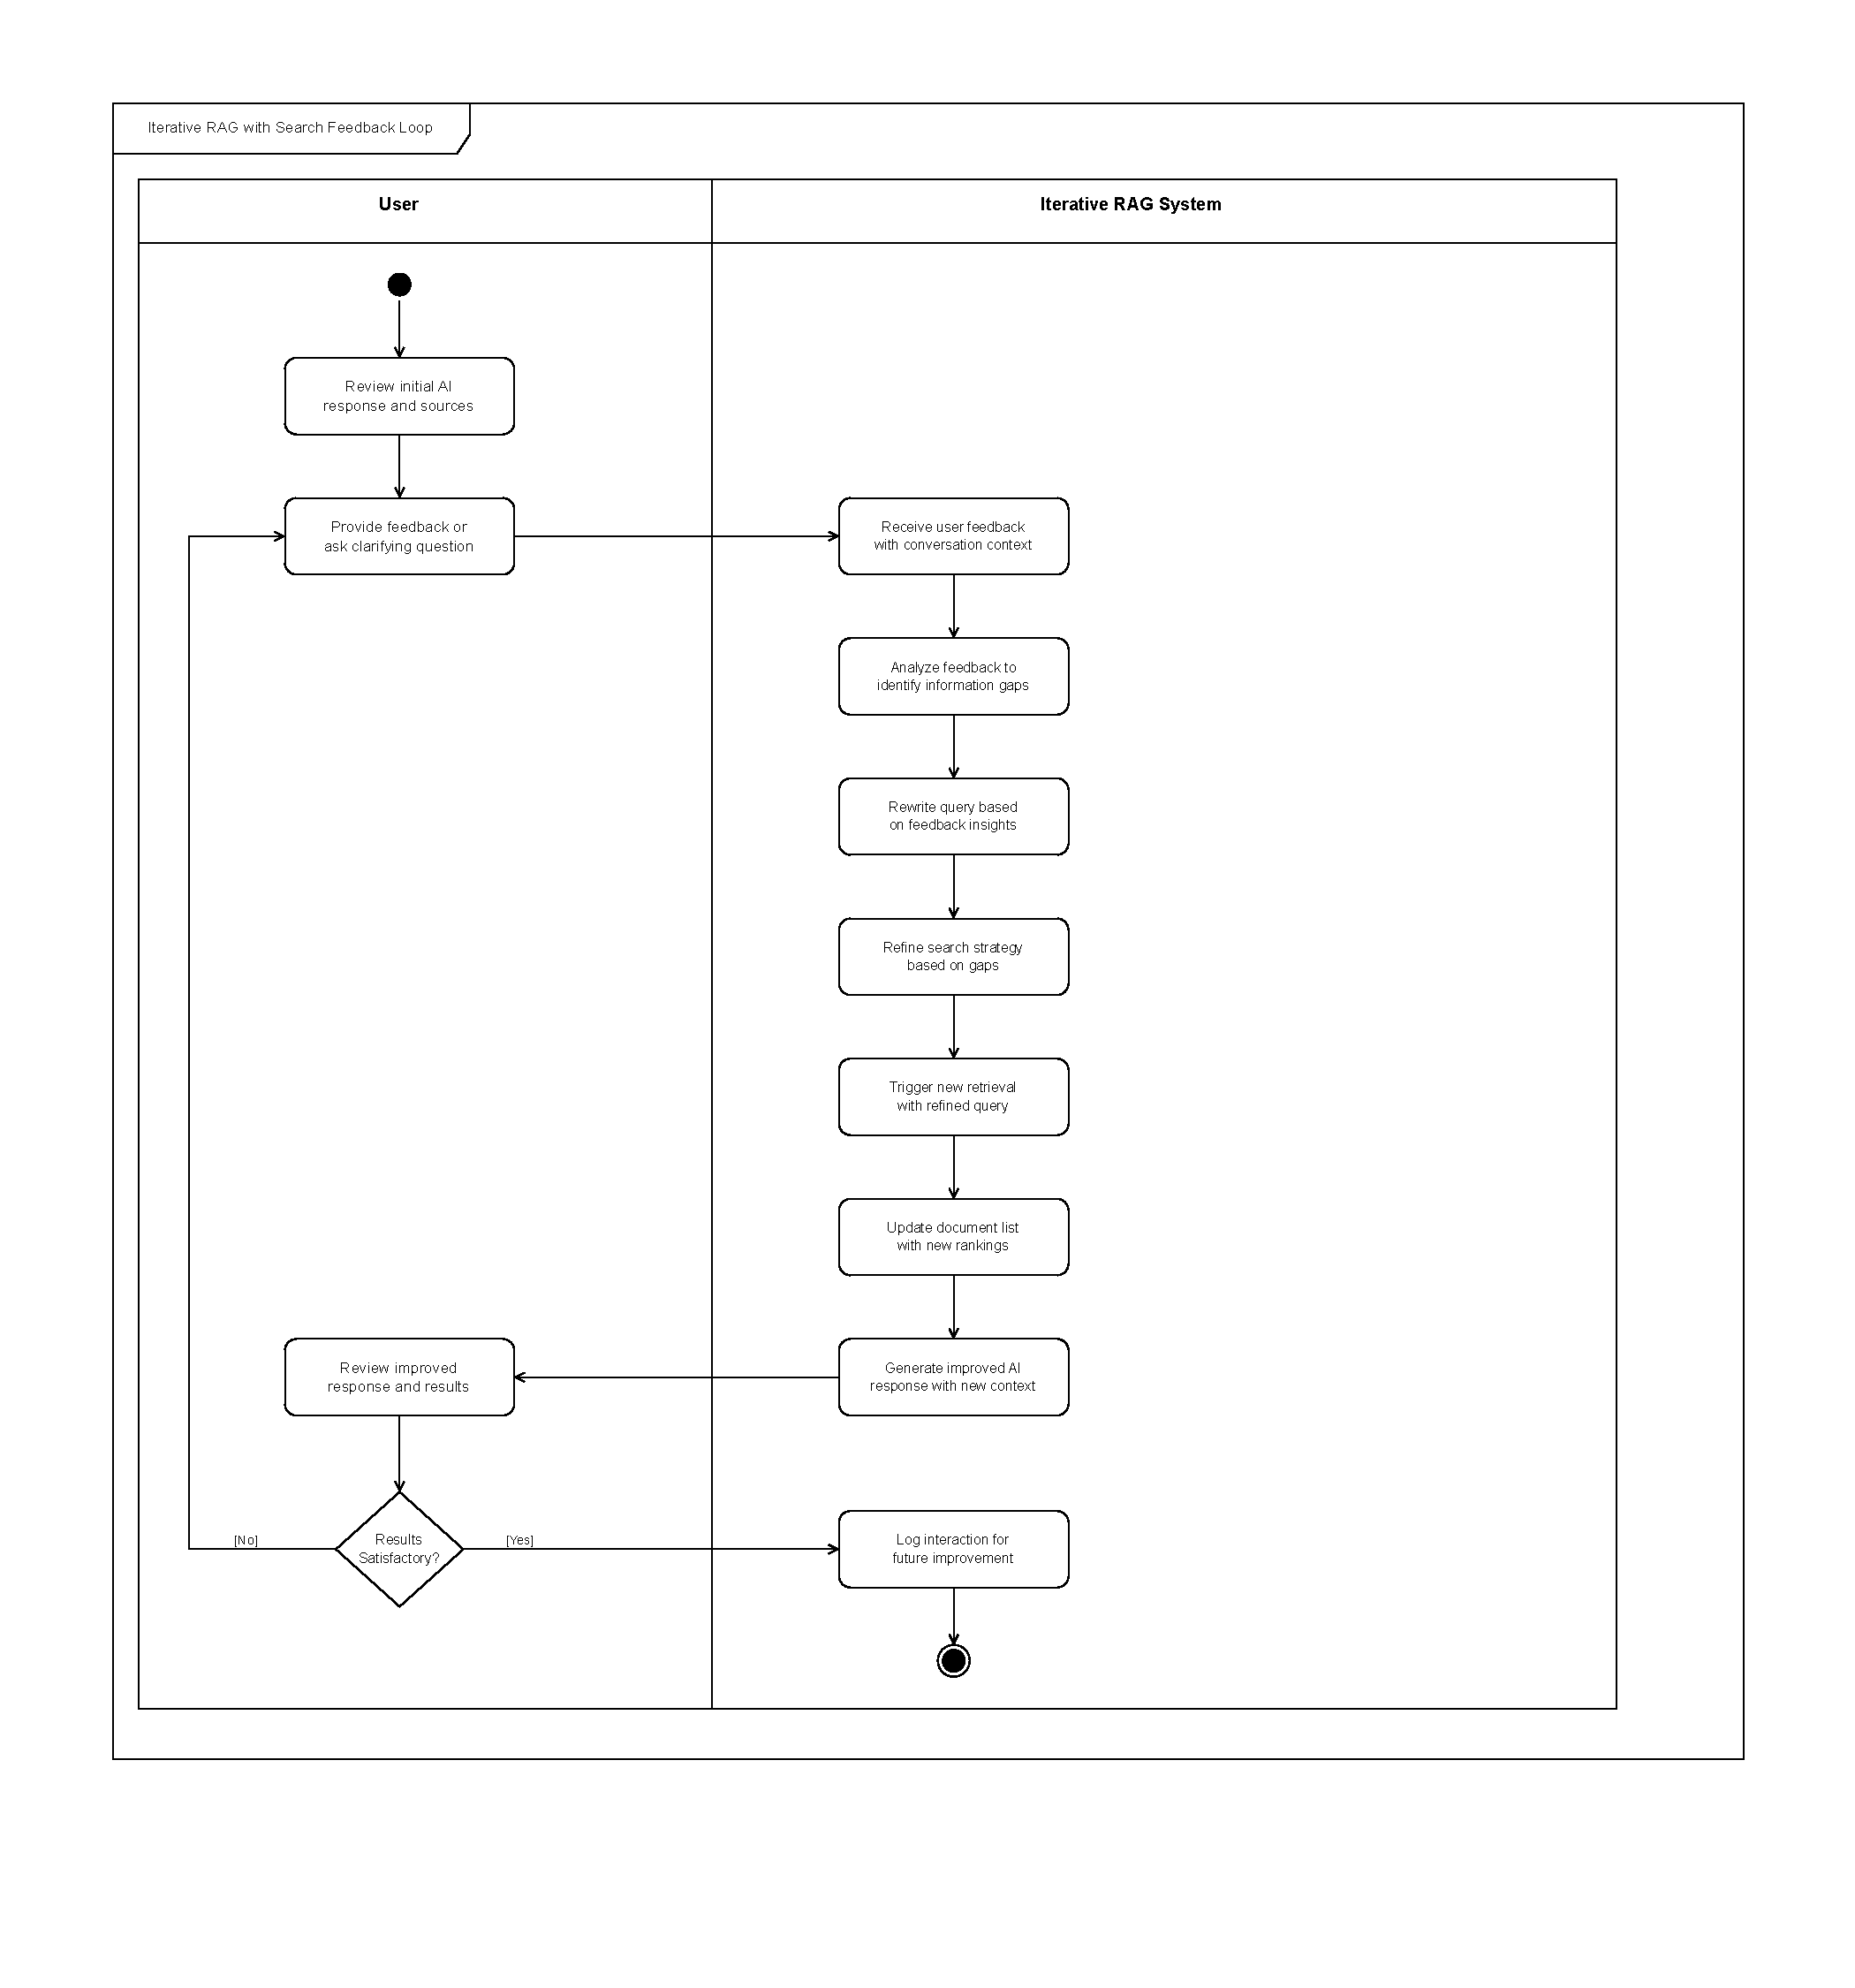
\includegraphics[width=0.55\linewidth]{activity10.drawio.pdf}
        \label{fig:placeholder}
    \end{figure}
\end{frame}

\begin{frame}{System Analysis and Design - Deployment Diagram}
    \begin{figure}
        \centering
        \vspace{-3px}
        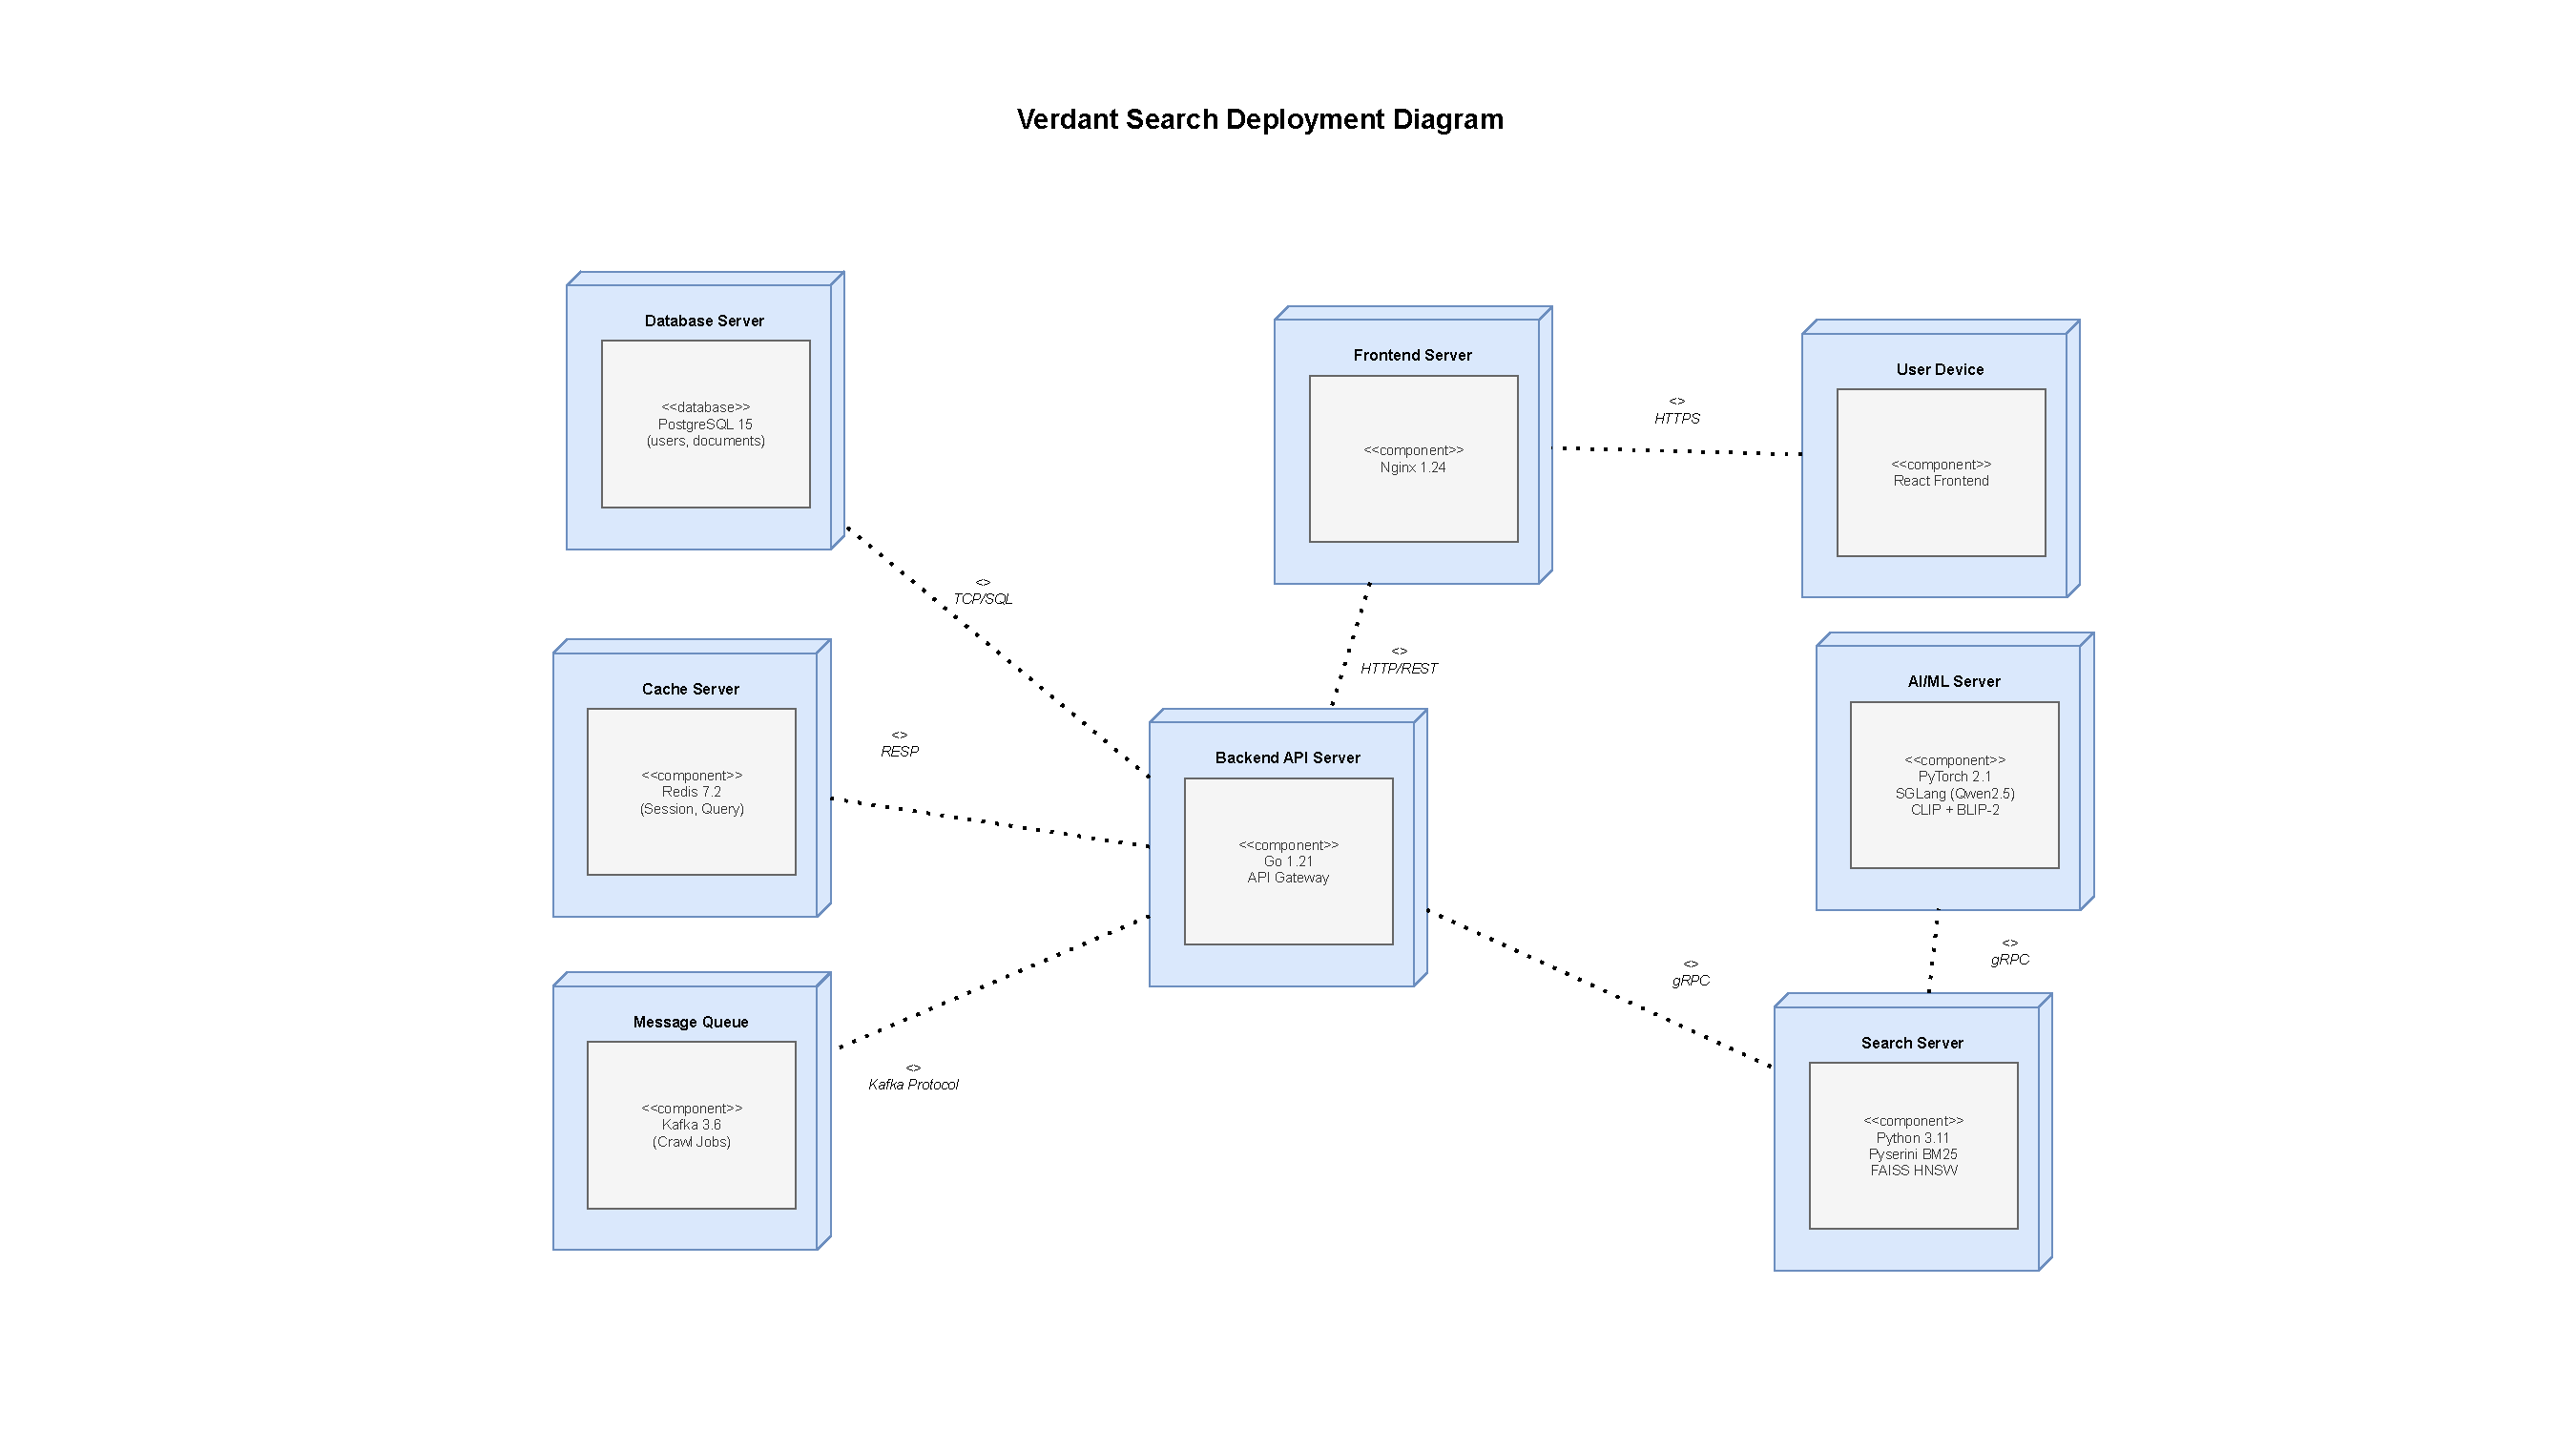
\includegraphics[width=1.0\linewidth]{deployment.drawio.pdf}
        \label{fig:placeholder}
    \end{figure}
\end{frame}

\begin{frame}{System Analysis and Design - Class Diagram}
    \begin{figure}
        \centering
        \vspace{-3px}
        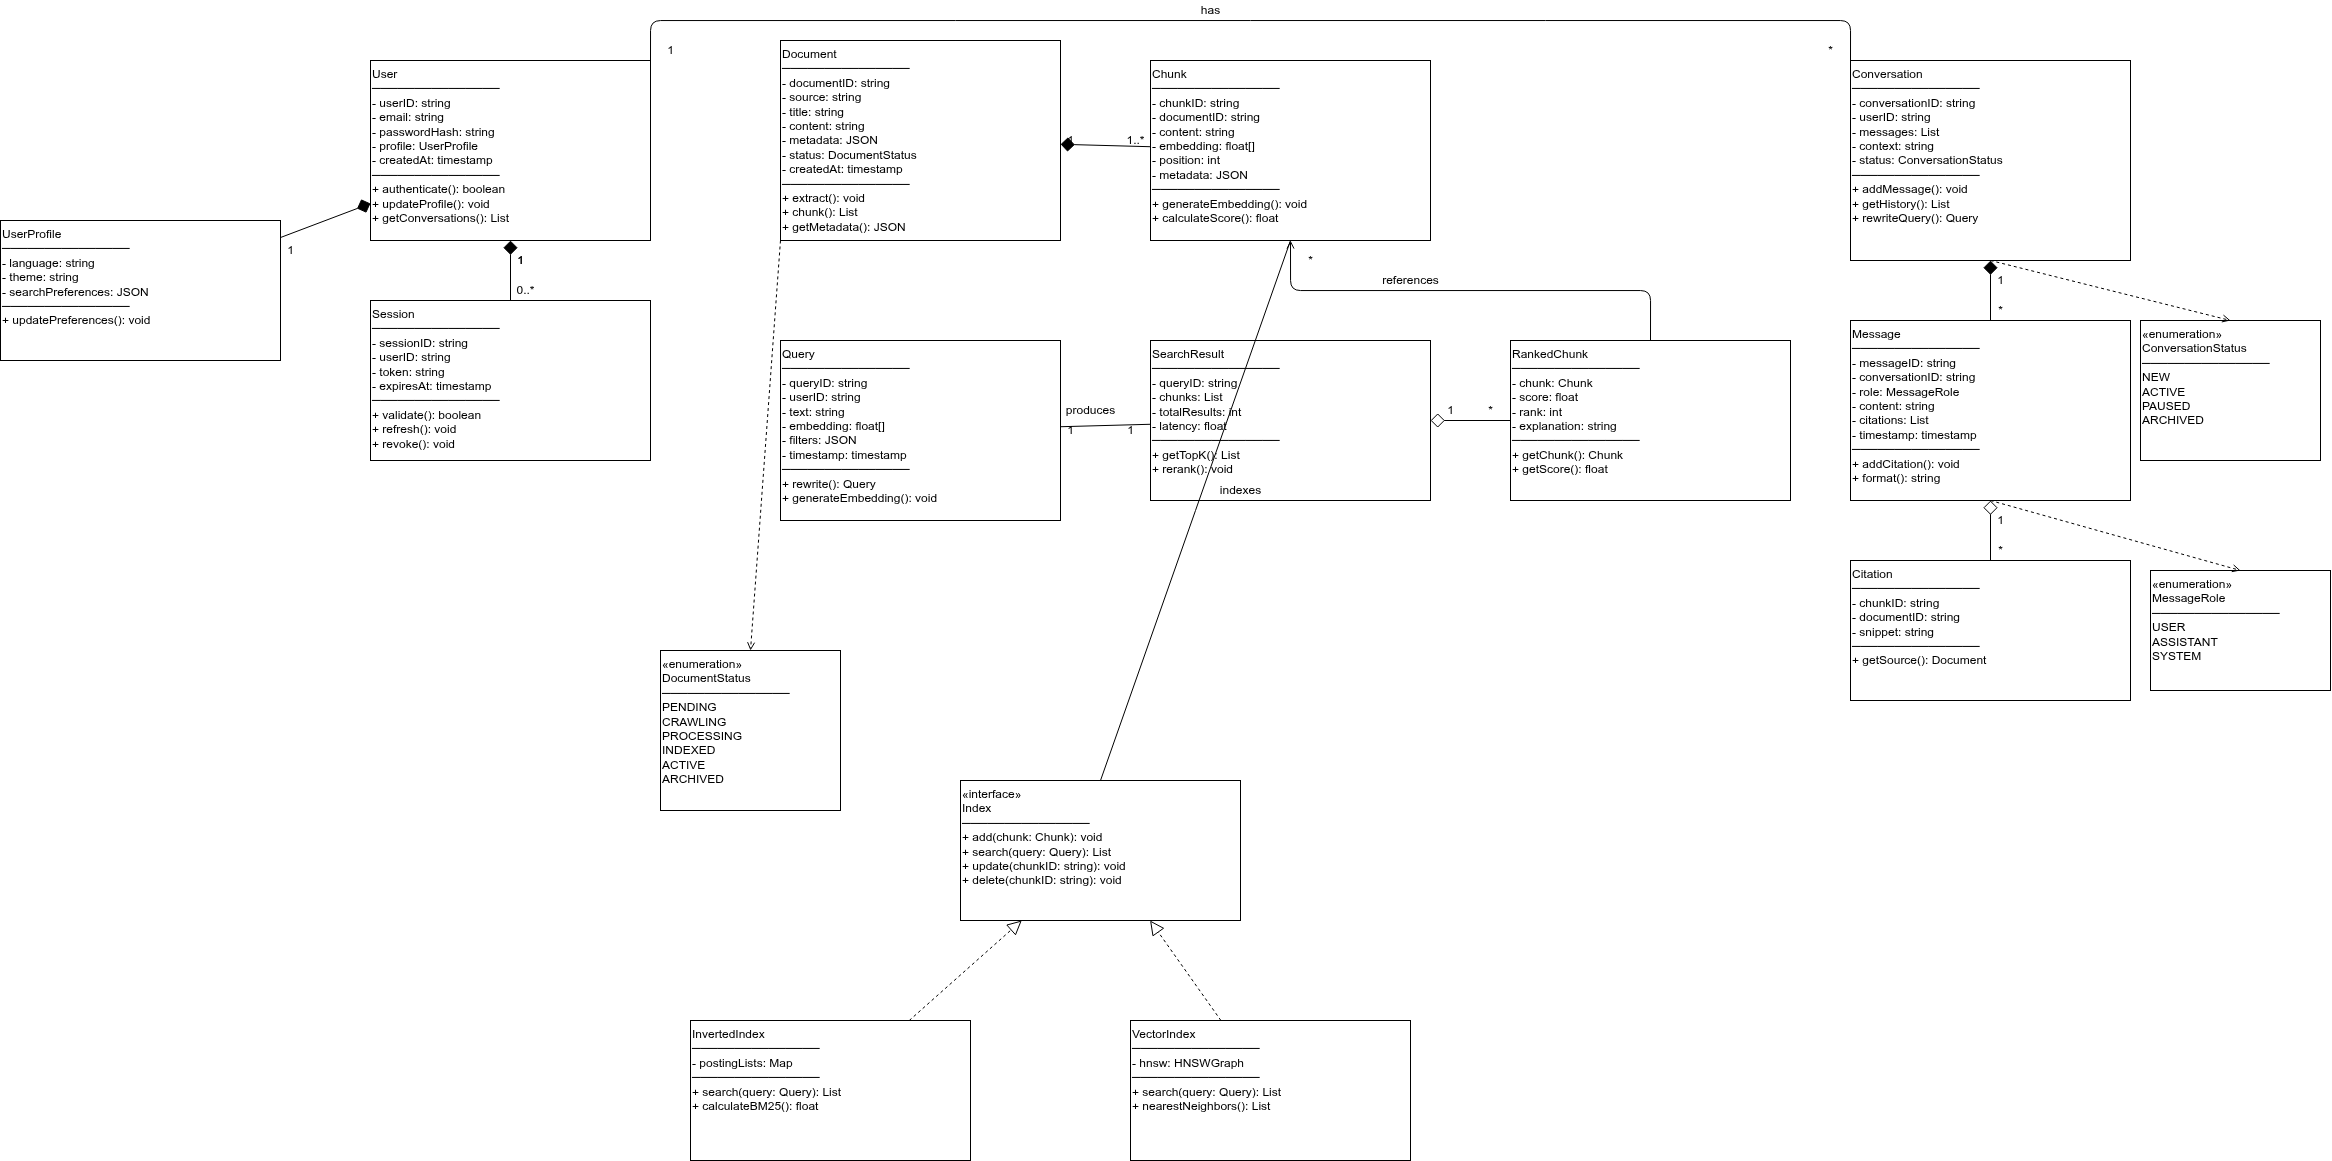
\includegraphics[width=1.0\linewidth]{class.drawio.png}
        \label{fig:placeholder}
    \end{figure}
\end{frame}

\begin{frame}{System Analysis and Design - Hardware Description}
    \small
    \begin{table}
        \centering
        \renewcommand{\arraystretch}{1.3}
        \begin{tabular}{p{0.25\textwidth}|p{0.65\textwidth}}
        \toprule
        \textbf{Component} & \textbf{Specification} \\
        \midrule
        \multicolumn{2}{c}{\textbf{Development Environment}} \\
        \midrule
        CPU & Intel Core i5-12450H (8 cores, 12 threads) \\
        \midrule
        RAM & 16GB DDR4 \\
        \midrule
        GPU & NVIDIA RTX 2080 Ti (11GB VRAM) \\
        \midrule
        Storage & 512GB NVMe SSD \\
        \midrule
        \multicolumn{2}{c}{\textbf{Model Training Environment (Company Server)}} \\
        \midrule
        CPU & Intel Core i9 (16 cores, 32 threads) \\
        \midrule
        RAM & 48GB DDR5 \\
        \midrule
        GPU & NVIDIA RTX 5090 (32GB VRAM) \\
        \midrule
        Storage & 2TB NVMe SSD \\
        \bottomrule
        \end{tabular}
    \end{table}
    
    \vspace{0.3em}
    \begin{block}{Training Configuration}
        Multimodal reranker model training performed on RTX 5090 with 32GB VRAM, enabling batch sizes up to 64 for efficient fine-tuning of BLIP-2 based architecture.
    \end{block}
\end{frame}

\begin{frame}{System Analysis and Design - User Interface Design (1/3)}
    \begin{figure}
        \centering
        \vspace{-3px}
        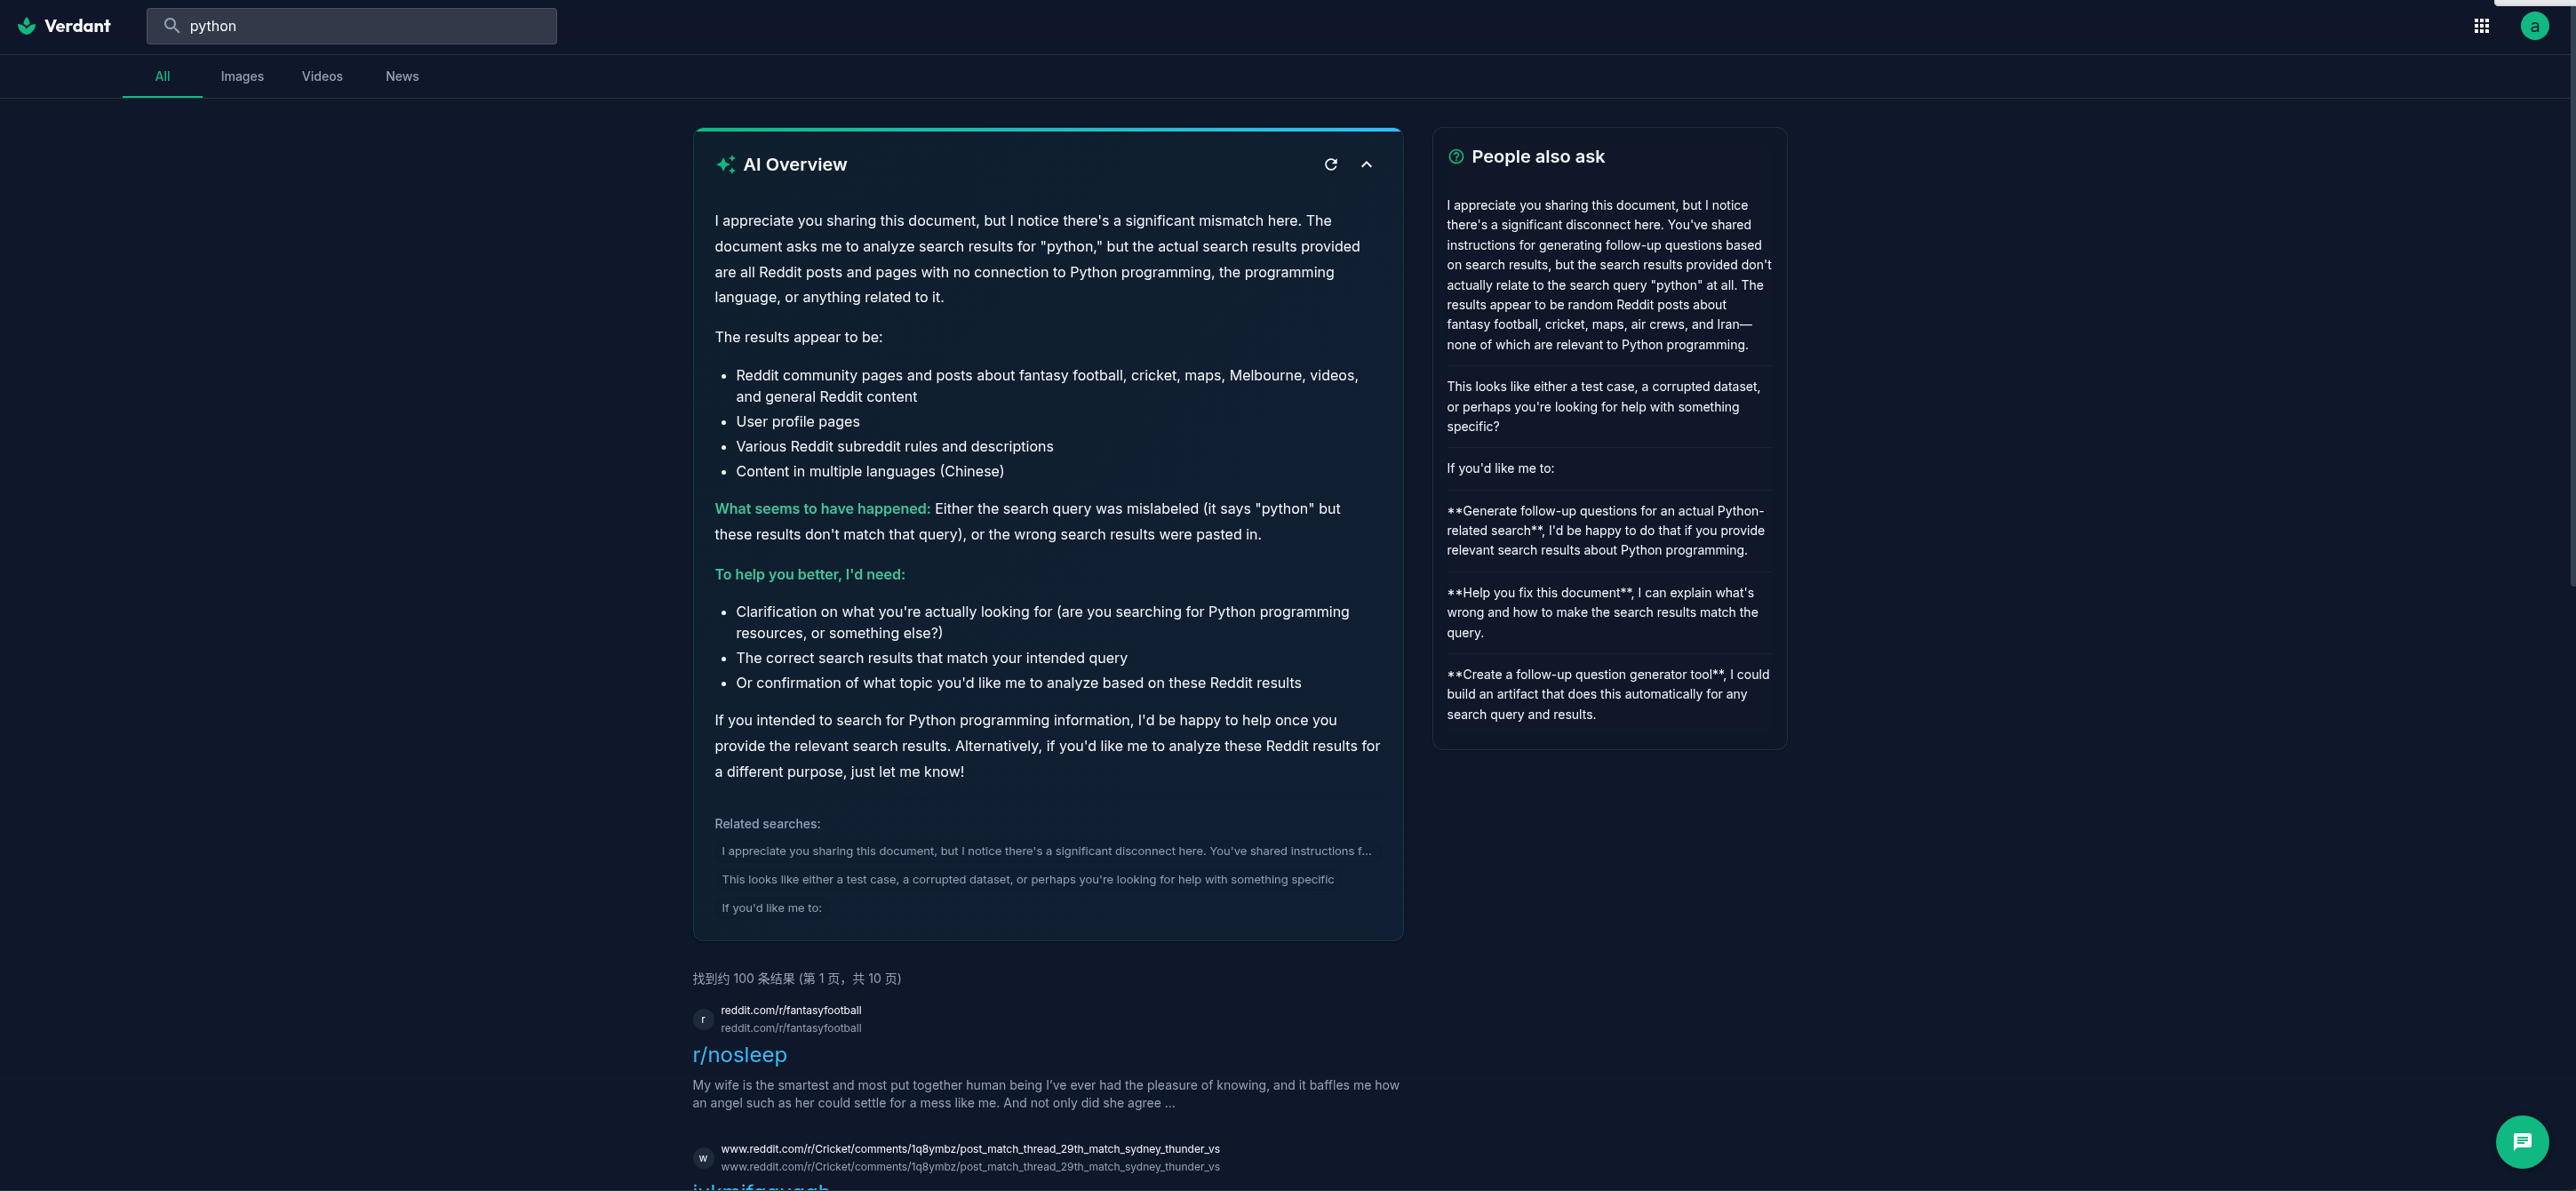
\includegraphics[width=0.95\linewidth]{ui_screenshot_1.png}
        \caption{Main Search Interface with Dual Panel Layout}
        \label{fig:ui1}
    \end{figure}
\end{frame}

\begin{frame}{System Analysis and Design - User Interface Design (2/3)}
    \begin{figure}
        \centering
        \vspace{-3px}
        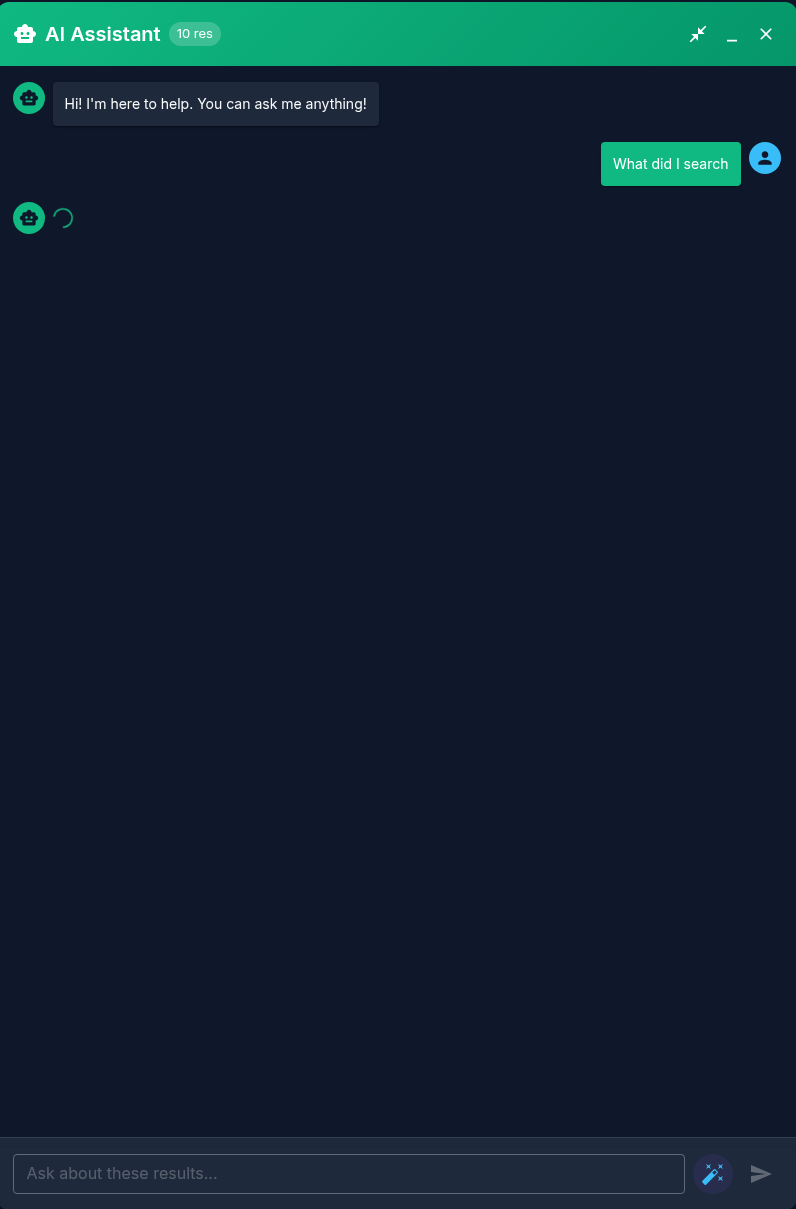
\includegraphics[height=0.75\textheight]{ui_screenshot_2.png}
        \caption{Search Results with Multimodal Content Display}
        \label{fig:ui2}
    \end{figure}
\end{frame}

\begin{frame}{System Analysis and Design - User Interface Design (3/3)}
    \begin{figure}
        \centering
        \vspace{-3px}
        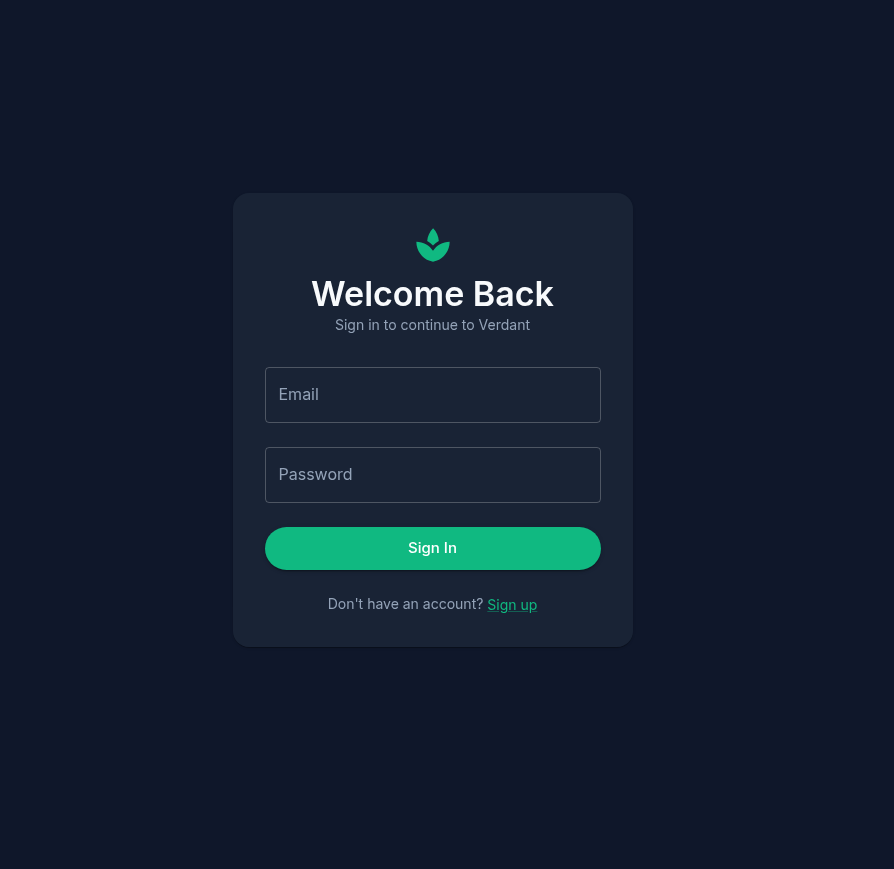
\includegraphics[height=0.75\textheight]{ui_screenshot_3.png}
        \caption{RAG Chat Interface with Citation and Source References}
        \label{fig:ui3}
    \end{figure}
\end{frame}

%------------------------------------------------
\section{Technical Implementation}
%------------------------------------------------

\begin{frame}{Technical Stack}
    \begin{columns}[t]
        \column{.48\textwidth}
        \textbf{Backend Technologies}
        \begin{itemize}
            \item \textbf{Core:} Golang for high performance concurrent processing
            \item \textbf{Database:} PostgreSQL for metadata and user data
            \item \textbf{Cache:} Redis for session management and query caching
            \item \textbf{Message Queue:} Kafka for distributed crawling coordination
            \item \textbf{Monitoring:} Prometheus and Grafana for observability
            \item \textbf{Retrieval:} Pyserini (BM25), FAISS/HNSW (vector search)
        \end{itemize}
        
        \column{.48\textwidth}
        \textbf{Frontend Technologies}
        \begin{itemize}
            \item \textbf{Framework:} ReactJS for dual panel interactive interface
            \item \textbf{Styling:} TailwindCSS for responsive design
            \item \textbf{Components:} Shadcn for accessible UI components
            \item \textbf{Static Site:} Astro for documentation and landing pages
        \end{itemize}
        
        \vspace{0.5em}
        \textbf{AI/ML Technologies}
        \begin{itemize}
            \item \textbf{Framework:} PyTorch for model training and inference
            \item \textbf{Serving:} SGLang for efficient LLM serving
            \item \textbf{Models:} CLIP, BLIP 2, custom multimodal LTR
        \end{itemize}
    \end{columns}
\end{frame}

\begin{frame}{Implementation Highlights}
    \begin{columns}[t]
        \column{.48\textwidth}
        \textbf{Key Innovations}
        \begin{itemize}
            \item Multimodal listwise reranking extending RankZephyr setwise prompting
            \item Closed loop RAG: LLM insights feed back into retrieval
            \item Efficient HNSW for subsecond ANN search on image embeddings
            \item Query rewriting for conversational context understanding
        \end{itemize}
        
        \column{.48\textwidth}
        \textbf{Optimization Strategies}
        \begin{itemize}
            \item Two stage ranking: Fast first stage, expensive reranking only on top K
            \item Incremental index updates to avoid full rebuilds
            \item Redis caching for frequently accessed documents
            \item Kafka based distributed crawling with coordinated deduplication
        \end{itemize}
    \end{columns}
\end{frame}

%------------------------------------------------

\begin{frame}
    \Huge{\centerline{\textbf{Thank You!}}}
    
    \vspace{1cm}
    \Large{\centerline{Questions?}}
    
    \vspace{1cm}
    \normalsize
    \centerline{Verdant Search: AI Boosted Sharded Distributed Search Engine}
    \centerline{CAI HONGYI, S2175463 | Supervisor: CHIAM YIN KIA}
\end{frame}

%----------------------------------------------------------------------------------------

\begin{frame}[t,allowframebreaks]{References}
    \tiny
    \printbibliography[heading=none]
\end{frame}

\end{document}